% FIT VUT
% Diplomová práce
% Autor: Jakub Sadílek
% Rok: 2021/2022

\colorlet{punct}{red!60!black}
\definecolor{delim}{RGB}{20,105,176}
\definecolor{codeblue}{rgb}{0,0,1}

\lstdefinelanguage{json}{
    basicstyle=\normalfont\ttfamily,
    numbers=left,
    numberstyle=\scriptsize,
    stepnumber=1,
    numbersep=8pt,
    showstringspaces=false,
    breaklines=true,
    literate=
     *{0}{{{\color{codeblue}0}}}{1}
      {1}{{{\color{codeblue}1}}}{1}
      {2}{{{\color{codeblue}2}}}{1}
      {3}{{{\color{codeblue}3}}}{1}
      {4}{{{\color{codeblue}4}}}{1}
      {5}{{{\color{codeblue}5}}}{1}
      {6}{{{\color{codeblue}6}}}{1}
      {7}{{{\color{codeblue}7}}}{1}
      {8}{{{\color{codeblue}8}}}{1}
      {9}{{{\color{codeblue}9}}}{1}
      {:}{{{\color{punct}{:}}}}{1}
      {,}{{{\color{punct}{,}}}}{1}
      {\{}{{{\color{delim}{\{}}}}{1}
      {\}}{{{\color{delim}{\}}}}}{1}
      {[}{{{\color{delim}{[}}}}{1}
      {]}{{{\color{delim}{]}}}}{1},
}

\definecolor{codegreen}{rgb}{0,0.6,0}
\definecolor{codeyellow}{rgb}{0.84,0.64,0.24}
\definecolor{codepurple}{rgb}{0.5,0.0,0.5}

\lstdefinelanguage{JavaScript}{
  keywords={const, typeof, new, true, false, catch, function, return, null, catch, switch, var, if, in, while, do, else, case, break},
  keywordstyle=\color{blue}\bfseries,
  ndkeywords={class, extends, export, boolean, throw, implements, import, this},
  ndkeywordstyle=\color{codepurple}\bfseries,
  identifierstyle=\color{black},
  sensitive=false,
  comment=[l]{//},
  morecomment=[s]{/*}{*/},
  commentstyle=\color{purple}\ttfamily,
  stringstyle=\color{codegreen}\ttfamily,
  morestring=[b]',
  morestring=[b]"
}
\lstset{
   language=JavaScript,
   extendedchars=true,
   basicstyle=\footnotesize\ttfamily,
   numberstyle=\footnotesize,
   frame=single,
   numbersep=9pt,
   numbers=left,
   tabsize=2,
   breaklines=true,
   showtabs=false,
   captionpos=b
}


\chapter{Úvod}
Náplní této práce je vytvořit nástroj pro snadné zpracování videozáznamu za účelem detekce a~analýzy narušitelů ve sledované oblasti s~možností konfigurace. Praktickým příkladem využití může být záznam z~bezpečnostní kamery, kde neoprávněna osoba vnikne na soukromý pozemek nebo záznam z~veřejného prostranství s~přímým výhledem na odpadkový koš, ve kterém byl nalezen předmět spojený s~trestným činem. Zpětné dohledávání těchto osob pak v~obvykle dlouhých záznamech může zabrat nemalé množství času.

Hlavní snahou je tedy tento proces více automatizovat a~nabídnout uživateli nástroj, který bude lehce dostupný a~snadno použitelný. Takovým nástrojem je klient-server aplikace, kde uživatel nahraje svá data, nakonfiguruje způsob zpracování a~po zpracování záznamu mu budou zobrazeny všechny nálezy potencionálních narušitelů. V~aplikaci je implementována řada funkcí, které může uživatel v~tomto kontextu využít jako je např.~vymezení sledované oblasti a~zamezení tak detekce objektů, které se nachází mimo ni nebo identifikace osob podle jejich obličeje. Mezi další funkce pak patří sledování objektů, vykreslování stop, které znázorňují cestu odkud daný narušitel přišel, počítání všech nálezů~aj. Pro pokročilejší zpracování je pak možné využít možnost pro použití vlastního detektoru.

V následujícím textu kromě teorie jsou taktéž nastíněny i~praktické aspekty, se kterými bylo nutné se během vývoje vypořádat. Konkrétně v~následující kapitole~\ref{kap:teorie} je popsána problematika zpracování obrazu pomocí neuronových sítí. Kapitola je především zaměřena na detekci a~klasifikaci objektů v~obraze a~rozpoznávání osob podle obličeje. Jsou zde uvedeny i~některé modely, které se v~této oblasti aktivně používají. Kapitola~\ref{kap:technologie} je zaměřena na vybrané technologie, které byly použity při implementaci klientské a~serverové části aplikace, včetně komunikace mezi nimi. V~kapitole~\ref{kap:implementace} je uveden návrh celého řešení a~výsledná podoba aplikace, jenž je doplněna o~některé zajímavé implementační detaily. Dále je v~této části popsána implementace serveru a~proces zpracování videa. Poslední kapitola~\ref{kap:experimenty} je věnována experimentům nad reálnými daty a~následnému vyhodnocení celého systému z~hlediska výkonnosti.


\chapter{Neuronové sítě pro zpracování obrazu}
\label{kap:teorie}
Tato kapitola uvede čtenáře do oblasti neuronových sítí, kde na začátku jsou vysvětleny základní principy fungování sítě, její struktura a~způsob trénování. Jelikož se tato práce zaměřuje na zpracování obrazu, tak následně je část textu věnována konvolučním neuronovým sítím, které se právě k~tomuto účelu používají. Poté je nastíněna problematika detekce a~klasifikace objektů a~jsou blíže specifikovány páteřní sítě a~\emph{state-of-the-art} modely, které se v~této oblasti uplatňují. Dále jsou zmíněny vybrané metody pro detekci obličejů a~v~závěru této kapitoly se pak nachází některá řešení pro rozpoznávání osob podle obličeje a~sledování objektů.

\section{Teorie neuronových sítí}
Neuronové sítě~\cite{book:NNandDL} jsou známou technikou strojového učení inspirovanou fungováním lidského mozku. Základní jednotkou tohoto nervového systému jsou neurony, které jsou navzájem propojeny a~jejich účelem je analyzovat a~vyhodnocovat data okolo nás. V~neuronových sítích jsou elementární výpočetní jednotkou \emph{umělé} neurony, jenž simulují vlastnosti těch reálných. Přestože výpočetní technologie excelují nad člověkem při řešení matematických výpočtů, nelze je tak snadno využít na úlohy, které jsou naopak triviální pro lidský mozek jako může být například rozpoznávání. Tyto úlohy totiž není možné lehce algoritmizovat, proto se neuronové sítě používají zejména tam kde:
\begin{itemize}
    \item model je velmi komplexní a~náročný předem algoritmizovat,
    \item v~závislosti na datech se chování programu postupem času mění,
    \item pro danou situaci nejsou předem známé všechny možnosti, které mohou nastat.
\end{itemize}

\subsection{Neuron}
\label{sec:Neuron}
Základní stavební jednotkou~\cite{book:NNandDL} neuronové sítě je neuron, jehož schéma je zobrazeno na obrázku~\ref{img:Neuron}. Neuron přijímá několik vstupů \emph{x}, které mají vlastní váhy \emph{w}. Váhy lze přirovnat ke \emph{\uv{zkušenostem}} a~čím je hodnota váhy vyšší, tím je daný vstup pro výpočet důležitější. Proces vyhodnocení probíhá tak, že na každém vstupu se hodnota s~váhou vynásobí a~jejich následný součet poslouží jako vstup do aktivační (přenosové) funkce, která spočítá výslednou hodnotu. Funkci tohoto modelu je možné popsat následující rovnicí~\ref{eqn:neuron}.

\begin{equation}
    \label{eqn:neuron}
    f(x) = \delta(\sum_{i=1}^{N}(x_i \cdot w_i) + b),
\end{equation}
kde \emph{f(x)} je výstupní hodnota neuronu, $\delta$ je aktivační funkce, \emph{N} je počet vstupů, \emph{x} je hodnota vstupu, \emph{w} je váha vstupu a~\emph{b} je bias neboli posunutí.

\begin{figure}[hbt]
	\centering
	\setlength{\fboxsep}{0pt}
	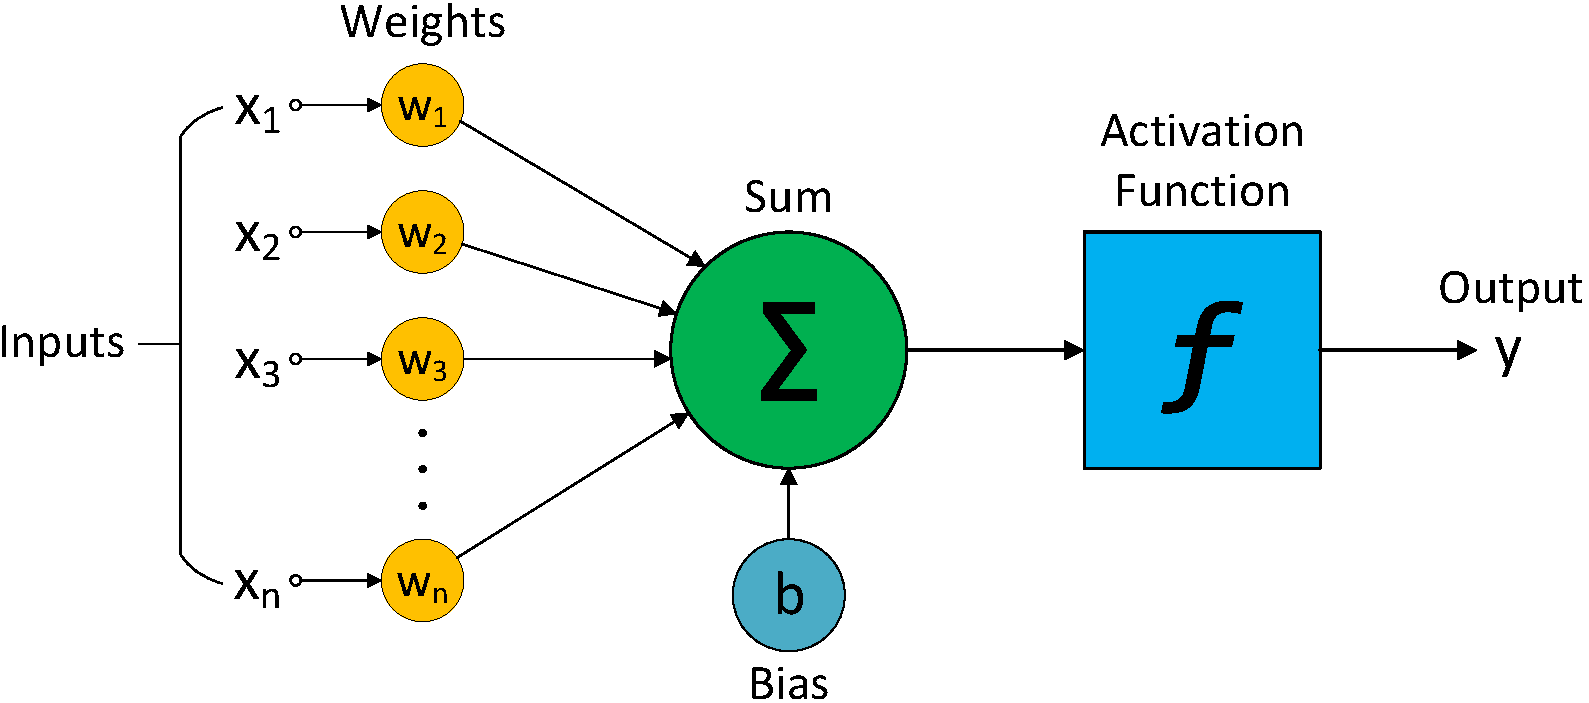
\includegraphics[width=0.78\textwidth]{obrazky-figures/neuron.pdf}
	\caption{Schéma neuronu s~biasem. Převzato z~knihy~\cite{book:NNandDL}.}
	\label{img:Neuron}
\end{figure}

Účelem \textbf{aktivační funkce} je zavést do váženého součtu nelinearitu, která bude produkována na výstup neuronu. Tento krok~\cite{website:IntroToNN} je důležitý zejména proto, že většina dat z~reálného světa má nelineární průběh a~cílem je neurony tuto nelineární reprezentaci naučit. V~praxi~\cite{website:OverviewOfActivationFunctions} se vyskytuje více druhů těchto funkcí, mezi tradiční patří například sigmoida nebo tanh (viz~obrázek~\ref{img:functions}). \textbf{Sigmoida} je příkladem logistické funkce, která se používá pro transformaci hodnot do intervalu <0, 1> a~využívá se pro vyjádření míry pravděpodobnosti. Název funkce vychází z~jejího tvaru do písmene \emph{S} a~je definována vztahem~\ref{eqn:sigmoid}. Funkce \textbf{tanh} neboli hyperbolický tangens lze chápat spíše jako rozšíření sigmoidy, která má podobný tvar, ale produkuje výstup v~rozmezí <-1, 1> (viz~vzorec~\ref{eqn:tanh}).
\begin{equation}
    \label{eqn:sigmoid}
    \sigma(x) = \frac{1}{1 + e^{-x}}
\end{equation}
\begin{equation}
    \label{eqn:tanh}
    tanh(x) = \frac{e^x - e^{-x}}{e^x + e^{-x}}
\end{equation}

Dále se často používá funkce \textbf{softmax}, která je zobecněním logistické funkce do více dimenzí a~je definována ve vzorci~\ref{eqn:softmax}. Využívá se především u~klasifikačních úloh v~poslední vrstvě, jejímž cílem je přiřadit prvek do jedné z~více předem definovaných tříd. Funkce přijímá vektor hodnot, který následně převede na vektor hodnot mezi 0 a~1, kde hodnota po součtu je rovná právě 1. Hodnoty tak reprezentují pravděpodobnost příslušnosti prvku k~daným třídám.
\begin{equation}
    \label{eqn:softmax}
    softmax(x_i) = \frac{e^{x_i}}{\sum_{j=1}^{N}e^{x_j}}
\end{equation}
    
Nejčastěji však používanou \emph{moderní} funkcí je \textbf{ReLU} \emph{(Rectified Linear Unit)}~\cite{website:OverviewOfActivationFunctions}, která kladné hodnoty propaguje přímo na výstup, zatímco záporné hodnoty kompletně eliminuje na nulu~--~viz~matematická definice~\ref{eqn:relu} a~její průběh na obrázku~\ref{img:functions}. Tato funkce se stala populární díky svému výkonu v~podobě méně operací a~menšímu problému s~mizejícím gradientem v~porovnání s~výše zmíněnými funkcemi, čímž zapříčiňuje vysokou míru učenlivosti modelu. Funkce však s~sebou přináší problém, kdy při záporných hodnotách učení stagnuje kvůli nulovému gradientu (tento jev se nazývá \emph{\uv{dying ReLU problem}}). Problém řeší její upravená verze \textbf{Leaky ReLU}~\cite{website:OverviewOfActivationFunctions}, která při záporné hodnotě propaguje pouze hodnotu velmi blízké nule a~neuron tak musí neustále reagovat. 
\begin{equation}
    \label{eqn:relu}
    ReLU(x) = max(0, x)
\end{equation}

\begin{figure}[hbt]
	\centering
	\setlength{\fboxsep}{0pt}
	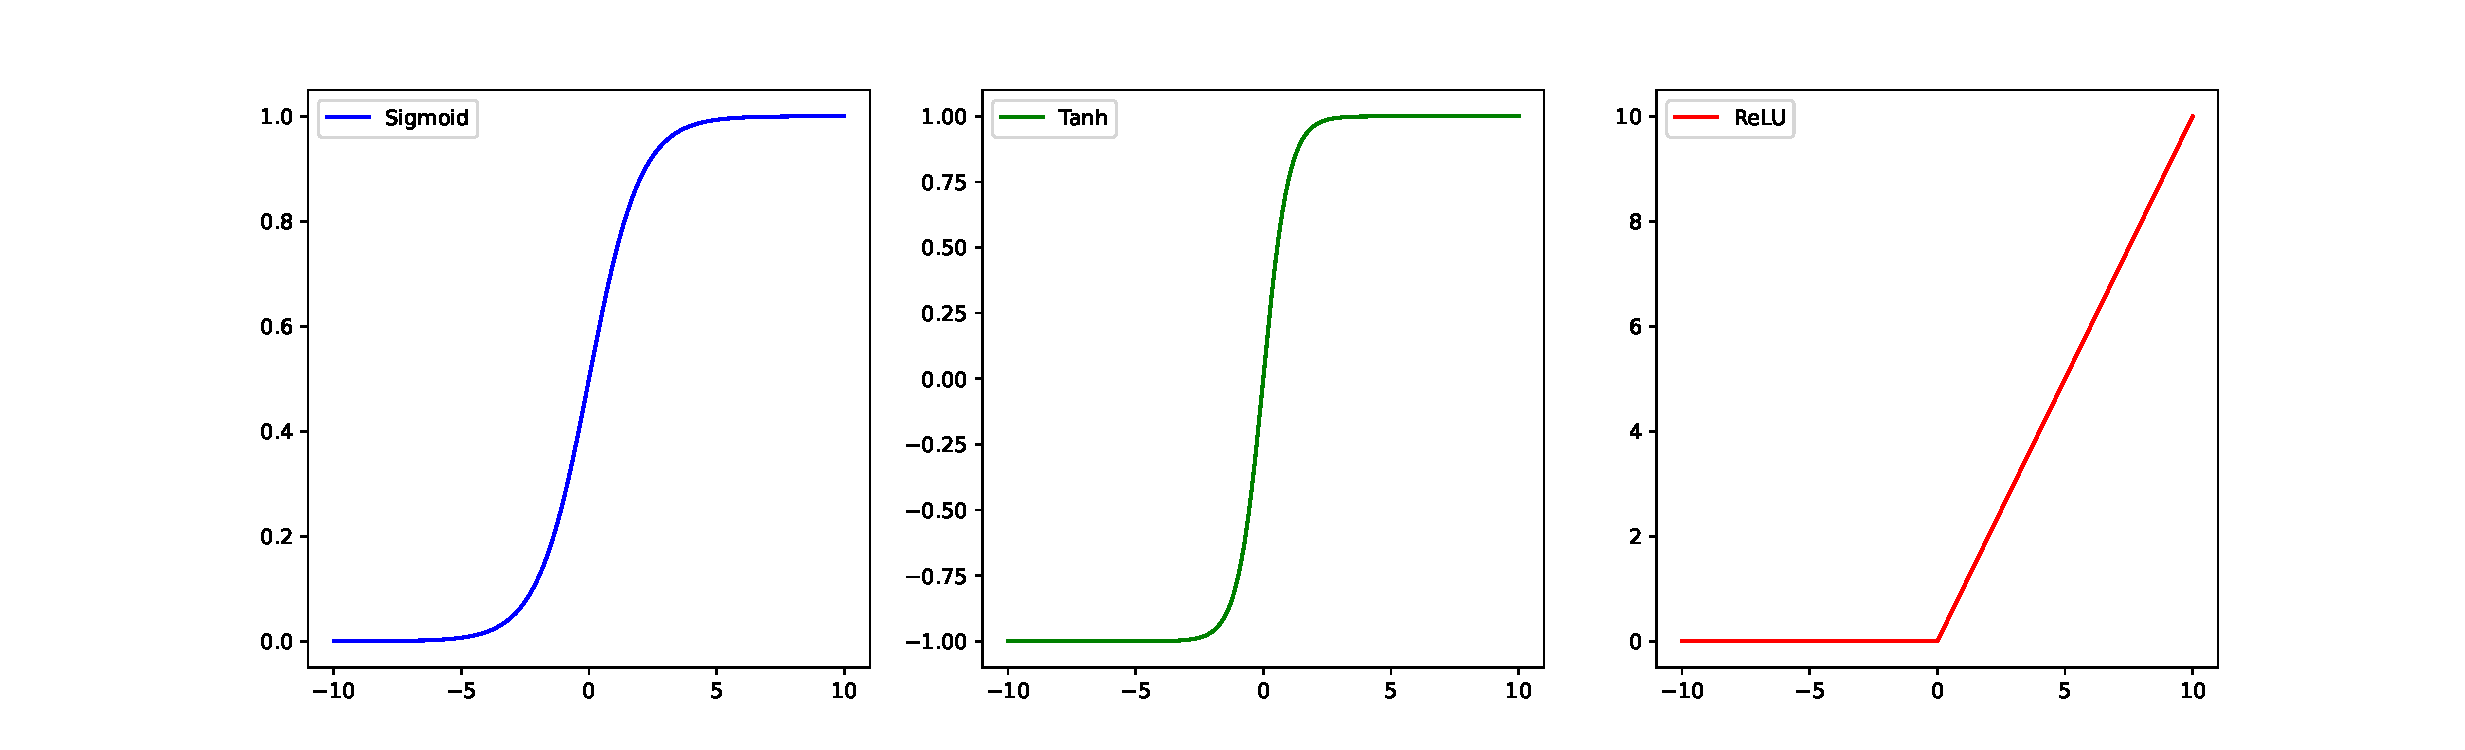
\includegraphics[width=1.0\textwidth]{obrazky-figures/actFunctions.pdf}
	\caption{Graf průběhů aktivačních funkcí, kde vlevo se nachází sigmoida, uprostřed tanh a~vpravo ReLU.}
	\label{img:functions}
\end{figure}

\subsection{Vrstvy a~učení neuronové sítě}
Stejně jako v~lidském mozku, tak i~v~neuronových sítích jsou neurony mezi sebou propojeny. V~neuronové síti jsou neurony koncipovány ve vrstvách, které jsou na sebe napojeny a~mohou obsahovat libovolný počet neuronů. První vrstva se nazývá vstupní a~definuje rozměry vstupního vektoru, zatímco výstup ze sítě je produkován poslední vrstvou, která se nazývá výstupní. Mezi vstupní a~výstupní vrstvou se může nacházet několik skrytých vrstev, jejichž počet určuje hloubku neuronové sítě.

K tomu~\cite{website:NNForBeginnersByBeginner}, aby byla síť schopna produkovat správné výsledky, musejí vrstvy implementovat funkci pro \textbf{dopřednou propagaci} \emph{(forward propagation)} a~k~tomu, aby byla schopna se učit, tak implementovat funkci pro \textbf{zpětnou propagaci} \emph{(backward propagation)}. Proces zpracování dat potom probíhá tak, že data ze vstupní vrstvy se přenáší přes skryté vrstvy, kde pomocí funkce dopředné propagace a~následnému zavedení nelinearity se postupně dostanou až do výstupní vrstvy. Během této propagace se neděje žádné učení a~účelem je pouze provést predikci nad vstupními daty a~následně reprezentovat výsledek. Zpětná propagace probíhá opačným směrem a~jejím účelem je zlepšit přesnost sítě (učit ji) upravením jejích vah. Míra úpravy je provedena v~závislosti na hodnotě učícího koeficientu a~podle toho, jak moc byl výsledek rozdílný vůči očekávanému výstupu \emph{(ground truth)}. Typy učení se dělí následovně:
\begin{itemize}
    \item \textbf{Učení s~učitelem} \emph{(supervised learning)}~--~v~tomto typu učení jsou vstupní data poskytnuta zároveň s~očekávaným výstupem pomocí tzv.~\emph{labels}.
    \item \textbf{Učení bez učitele} \emph{(unsupervised learning)}~--~zde jsou poskytnuta pouze vstupní data a~síť musí sama zjistit správný výstup bez jakéhokoliv vnějšího zásahu. 
    \item \textbf{Posilované učení} \emph{(reinforcement learning)}~--~tento přístup využívá k~ohodnocení korektnosti výstupu tzv.~odměny, jenž udávají pouze míru toho, jak byl výsledek správný. Využívá se například u~hraní her, kdy správný tah je ohodnocen kladným skóre a~špatný tah záporným.
\end{itemize}

K zjištění míry~\cite{website:NNForBeginnersByBeginner} toho, jak daleko byl model od správného výsledku se používá tzv.~\textbf{ztrátová funkce} \emph{(loss function)}. Ačkoliv existuje mnoho druhů těchto funkcí, tak slouží ke stejnému účelu a~její výběr se odvíjí podle účelu vyvíjeného modelu. Známou variantou je například funkce střední kvadratické chyby \emph{(mean squared error)}. Úspěšnost modelu je pak definována \textbf{nákladovou funkcí} \emph{(cost function)}, která udává chybu nad celým datasetem průměrováním jednotlivých hodnot loss funkcí. Během tréninku je tak cílem dosáhnout minimální hodnoty cost funkce, aby predikce modelu byly co nejpřesnější.

K minimalizaci chyby cost funkce~\cite{website:NNForBeginnersByBeginner} se používají \textbf{optimalizátory}. Ty pomocí vah upravují model do lepší formy v~závislosti na hodnotách loss funkce. Díky tomu model neustále zlepšuje své predikce a~postupně konverguje do ideální podoby. Opět zde existuje spousta algoritmu a~mezi nejznámější patří např.~gradientní sestup \emph{(gradient descent)}, jehož reprezentaci lze vidět na obrázku~\ref{img:GradientDescent}.

Účelem algoritmu pro \textbf{gradientní sestup}~\cite{website:NNForBeginnersByBeginner} je dosáhnout lokálního minima pomocí jednotlivých kroků, jejichž velikost je dána hyperparametrem pro nastavení rychlosti učení \emph{(learning rate)}. Tento parametr má významný dopad na průběh učení, kde příliš velký koeficient způsobí velké kroky, které mohou zapříčinit přeskočení minima. Na druhou stranu příliš malé ohodnocení bude vyžadovat velké množství času a~výpočetního výkonu na dosažení uspokojivého výsledku.

Potom co doběhne zpětná propagace, zahájí se další cyklus učení s~novými vzorky přes dopřednou propagaci, kde by tentokrát měl model vykonat o~trochu lepší predikci. Tento proces probíhá, dokud není trénování dokončeno a~nalezeno minimum. Etapa, v~niž jsou právě jednou zpracována všechna data z~datasetu se nazývá \uv{epocha}. Epochu pak lze pro trénování rozdělit na menší části datasetu, které se nazývají \emph{\uv{batche}}.

\begin{figure}[hbt]
	\centering
	\setlength{\fboxsep}{0pt}
	\includegraphics[width=0.7\textwidth]{obrazky-figures/GradientDescent.png}
	\caption{Znázornění algoritmu pro gradientní sestup, jenž v~prvním kroku získá aktuální sklon funkce pomocí derivace prvního řádku v~aktuálním bodě. Následně provede krok v~opačném směru růstu gradientu pro nalezení lokálního minima. Převzato z~článku~\cite{website:NNForBeginnersByBeginner}.}
	\label{img:GradientDescent}
\end{figure}

\section{Konvoluční neuronové sítě}
Konvoluční neuronové sítě (KNN)~\cite{website:CNNOverviewAndApplication} jsou typem neuronových sítí, které se používají pro zpracování obrazových dat. Tyto sítě jsou navrženy tak, aby nemusely v~obraze počítat s~každým pixelem jako s~odlišnou informací, ale spíše se naučily rozeznávat známé vzory, stejně tak, jak je to přirozené pro člověka. Obvykle se skládá z~konvolučních a~pooling vrstev, které provádějí extrakci příznaků. Plně propojené vrstvy, pak provádí klasifikaci a~převádí získané informace na výstupní vrstvu sítě~--~viz~následující obrázek~\ref{img:CNN}.

\begin{figure}[hbt]
	\centering
	\setlength{\fboxsep}{0pt}
	\includegraphics[width=1.0\textwidth]{obrazky-figures/CNNarchitecture.jpeg}
	\caption{Architektura KNN, kde na vstupní vrstvu je přiveden obrázek, ze kterého jsou následně extrahované příznaky pomocí konvolučních a~pooling vrstev. Nakonec jsou příznaky vektorizovány a~pomocí sekvence plně propojených vrstev je obrázek klasifikován. Převzato z~článku~\cite{website:ComprehensiveGuideToCNN}.}
	\label{img:CNN}
\end{figure}

\subsection{Konvoluční vrstva}
Konvoluční vrstva~\cite{website:CNNOverviewAndApplication} hraje v~KNN klíčovou roli, která provádí extrakci příznaků pomocí konvoluce, kde na vstupní data (obraz), reprezentována ve dvourozměrné matici se aplikuje malý filtr \emph{(kernel)}. Ve skutečnosti konvoluční vrstva může obsahovat více těchto filtrů, které extrahují různé vlastnosti a~jejich počet pak udává hloubku dané vrstvy. Výsledkem těchto operací je matice nazývaná mapa příznaků \emph{(feature map)}, jejíž hloubka se odvíjí od počtu použitých filtrů.

\begin{figure}[hbt]
	\centering
	\setlength{\fboxsep}{0pt}
	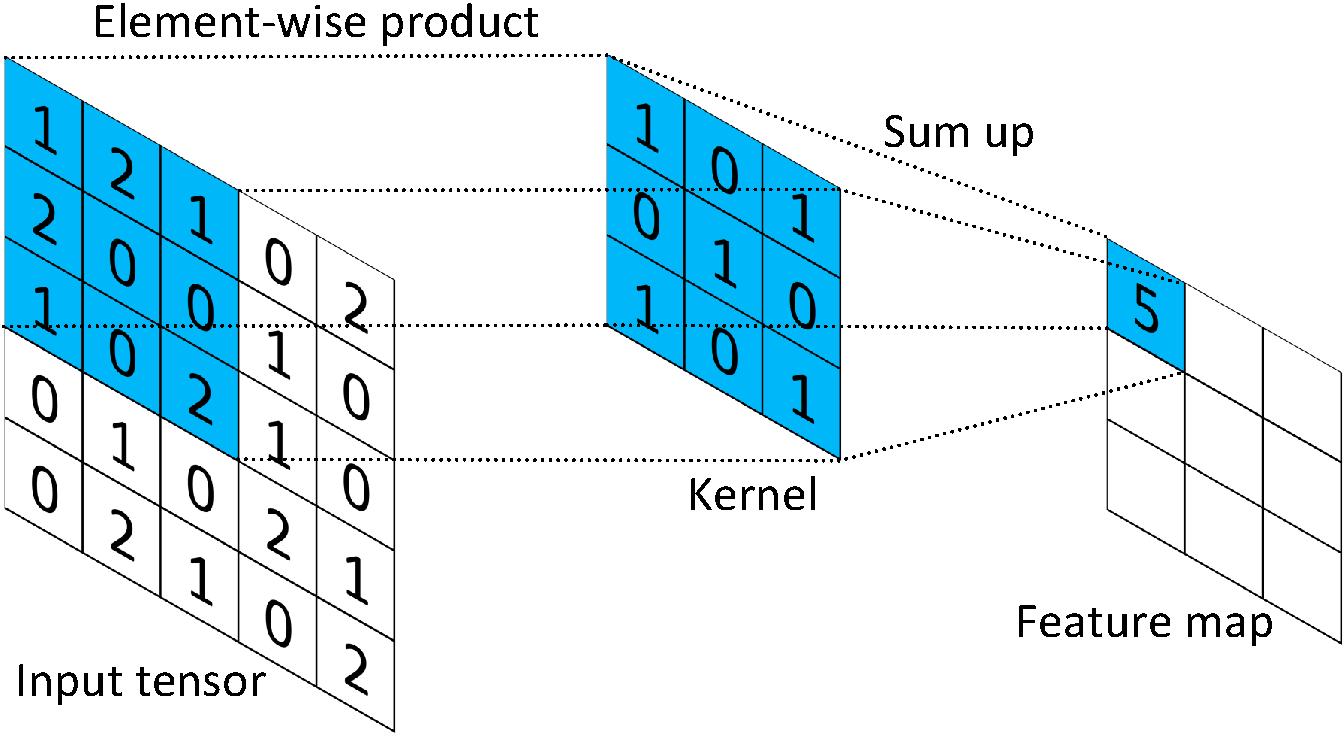
\includegraphics[width=0.67\textwidth]{obrazky-figures/convolution.pdf}
	\caption{Proces získání mapy příznaků pomocí konvoluce, kde aplikovaný filtr postupnými posuvy zpracuje celou vstupní matici a~produkuje mapu příznaků. Převzato z~článku~\cite{website:CNNOverviewAndApplication}.}
	\label{img:convolution}
\end{figure}

Každý filtr je složen z~trénovatelných vah a~také má vlastní hloubku, kterou přejímá od vstupních dat~--~např.~filtr pro zpracování RGB obrázku bude mít hloubku 3. Konvoluce pak probíhá posuvem filtru přes vstupní matici, kde v~každém kroku je spočítán jeden prvek výsledné mapy (viz~obrázek~\ref{img:convolution}). Velikost posuvu mezi kroky se nazývá \emph{stride} a~diskrétní 2D konvoluci lze popsat následujícím vztahem~\ref{eqn:knonvoluce}.
\begin{equation}
    \label{eqn:knonvoluce}
    y(m, n) = \sum_{i = 0}^{A - 1} \sum_{j = 0}^{B - 1} f(i, j) \cdot x(m - i, n - j),
\end{equation}
kde \emph{y} je výstupní matice, \emph{f} je použitý filtr, \emph{x} je vstupní matice, \emph{A} a~\emph{B} jsou rozměry filtru, \emph{m} a~\emph{n} jsou souřadnice aktuálně počítaného prvku ve výstupní matici. Kvůli pohybu filtru~\cite{website:CNNOverviewAndApplication} ve vstupní matici však není možné, aby střed filtru pokryl i~hraniční prvky této matice, což má za následek zmenšení výstupní mapy. K~řešení tohoto problému se používá tzv.~nulová výplň \emph{(zero-padding)}, která okraje vstupní matice vyplní nulami a~tím umožní střed filtru umístit i~na její nejkrajnější prvky. Díky této technice pak zůstane velikost výstupní mapy vůči vstupu zachována, a~je tak umožněno lépe aplikovat více filtrů. Nejvýznamnější dopad na proces trénování má však správná definice filtrů, které se nejvíce hodí na řešení daného úkolu. Filtry jsou pak jediné parametry v~této vrstvě, které se během procesu tréninku učí a~zlepšují predikci sítě. Na druhou stranu velikost filtrů, jejich počet, výplň a~stride jsou hyperparametry, které se nastavují před samotným procesem.

\subsection{Pooling vrstva}
Pooling vrstva~\cite{website:CNNOverviewAndApplication} poskytuje typickou operaci převzorkování (podvzorkování), která snižuje velikost dimenzí mapy příznaků. Účelem je zavedení translační invariance v~případě menších posunů a~snížení tak počtu trénovatelných parametrů, které se nachází v~konvolučních vrstvách. Hloubka ovšem zůstává nezměněna. Důležité však při tomto procesu je nějakým způsobem zachovat nejpodstatnější informace. Pooling vrstva sama o~sobě neobsahuje žádné trénovatelné parametry, kdežto obsahuje hyperparametry pro nastavení stride, výplně a~velikosti filtru obdobně jako u~konvoluční vrstvy.

Nejčastěji používaná pooling vrstva bývá tzv.~\emph{max-pooling} nebo \emph{average-pooling} vrstva s~rozměry filtru $2 \times 2$ a~nastaveném stride na 2 (viz~obrázek~\ref{img:pooling}). Max-pooling při filtraci příznaků propaguje prvek s~nejvyšší hodnotou a~ostatní eliminuje. Average-pooling vrstva zase produkuje průměrnou hodnotu ze všech hodnot z~aktuálního překryvu. Filtr se následně posune o~velikost stride dále.

\begin{figure}[hbt]
	\centering
	\setlength{\fboxsep}{0pt}
	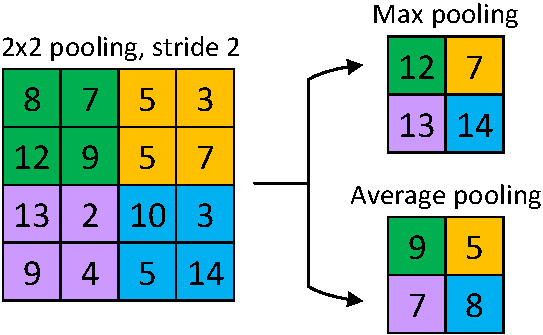
\includegraphics[width=0.5\textwidth]{obrazky-figures/pooling.pdf}
	\caption{Ukázka podvzorkování mapy příznaků pomocí \emph{max-pooling} a~\emph{average-pooling} filtrů s~rozměry $2 \times 2$ a~nastaveném stride na 2. Převzato z~článku~\cite{website:CNNOverviewAndApplication}.}
	\label{img:pooling}
\end{figure}

\subsection{Plně propojená vrstva}
Plně propojená vrstva~\cite{website:CNNOverviewAndApplication} se běžně vyskytuje u~konce celého procesu, kdy mapa příznaků je již zploštělá z~konečné konvoluční či pooling vrstvy do jednorozměrného pole (vektoru). V~této vrstvě je každý vstup propojen s~každým výstupem pomocí naučitelných vah a~biasu, které jsou následně transformovány aktivační funkcí (viz~předchozí sekce o~umělém neuronu~\ref{sec:Neuron}). Typicky jsou tak extrahované vzory předešlými konvolučními a~pooling vrstvami namapovány množinou plně propojených vrstev na výstupní vrstvu sítě. Konečná plně propojená vrstva u~klasifikačních úloh má pak počet výstupních uzlů rovný počtu klasifikačních tříd.

\section{Detekce a~klasifikace objektů}
Detekce a~klasifikace patří mezi nejčastější úlohy řešených pomocí neuronových sítí a~spadá do základů počítačového vidění. Raná detekce~\cite{article:SurveyOfObjectDetection} byla postavena na ručně vytvořených detektorech příznaků (viz~sekce~\ref{sec:DetekceObličeje}) jako je Viola-Jones, histogram orientovaných gradientů~aj. Přestože tyto metody fungovaly, tak byly poměrně pomalé a~nepřesné, což se změnilo při znovu-uvedení KNN a~hlubokého učení. Detekce a~klasifikace objektů pak nachází své uplatnění např.~u~řízení autonomních vozidel, rozpoznávání identit osob pro zvýšení bezpečnosti či k~lékařským účelům.

\subsection{Páteřní architektury}
Páteřní sítě \emph{(backbone)}~\cite{article:SurveyOfObjectDetection} jsou nejdůležitější komponentou pro detekci objektů. Tyto sítě mají za úkol ze vstupního obrazu extrahovat příznaky pro jejich další využití v~modelu v~podobě mapy příznaků. Níže jsou uvedeny některé milníkové a~často používané architektury v~moderních detektorech.

\subsubsection{Reziduální sítě}
Běžný postup~\cite{website:IntroToResNet, website:ResNetIntro} v~návrhu sítě pro řešení stále komplexnějších úloh vede k~dalšímu přidávání vrstev a~tím zvyšování hloubky sítě. Intuice spočívá v~tom, že další vrstvy se postupně učí složitějším rysům, a~tak hlubší síť poskytne lepší přesnost a~výkon. Ukázalo se ovšem, že u~tradičního modelu KNN existuje maximální práh hloubky, jak je znázorněno na obrázku~\ref{img:ResNetLayers}.

\begin{figure}[hbt]
	\centering
	\setlength{\fboxsep}{0pt}
	\includegraphics[width=1.0\textwidth]{obrazky-figures/ResNetLayers.png}
	\caption{Znázornění vztahu mezi hloubkou sítě a~jejím výkonem, kde hlubší síť vykazuje horší přesnost. Tento jev může být způsoben optimalizační funkcí, inicializací sítě nebo zejména problémem mizejícího (či explodujícího) gradientu. Převzato z~článku~\cite{article:DeepResNetForImg}.}
	\label{img:ResNetLayers}
\end{figure}

Tento problém~\cite{website:IntroToResNet, article:DeepResNetForImg} velmi hlubokých sítí se podařilo zmírnit zavedením reziduálních sítí (ResNets), které jsou tvořené speciálními vrstvami nazývané reziduální bloky (viz~obrázek~\ref{img:ResNetBlock}). Nejvýznamnější modifikací těchto bloků jsou tzv.~zkratky, které umožňují přeskočit jednu či více vrstev. Výhoda spočívá v~tom, že pokud nějaká vrstva zhoršuje výkon modelu, tak potom bude přeskočena (tj.~v~ideálním případě bude $F(x)$ na obr.~\ref{img:ResNetBlock} naučené na $0$). Zkratka~\cite{website:QuickOverviewResNet, website:ResNetIntro} se skládá z~tzv.~\uv{funkce mapování identity}, která se dělí na identitu a~projekci. \textbf{Identita} se používá v~případě, kdy data na vstupu a~výstupu bloku mají stejnou dimenzi, a~je tak možné data pouze předat bez jakékoliv modifikace. Vztah pro mapování identity je definován následujícím vzorcem~\ref{eqn:identita}.
\newpage
\begin{equation}
    \label{eqn:identita}
    y = \mathcal{F}(x, \{W_i\}) + x,
\end{equation}
kde $y$ je výstup, $x$ je vstup, $\mathcal{F}(x, \{W_i\})$ představuje reziduální mapování, jenž se má naučit, $W_i$ označuje váhu $i$-té vrstvy v~daném bloku. \textbf{Projekce}~\cite{website:QuickOverviewResNet} se naopak používá v~případě, kdy dimenze výstupu neodpovídá vstupu a~je tak nutné data přizpůsobit pomocí konvoluce. Vzorec je pak modifikován o~lineární projekci $W_s$ ve vztahu~\ref{eqn:projekce}.
\begin{equation}
    \label{eqn:projekce}
    y = \mathcal{F}(x, \{W_i\}) + W_s \cdot x
\end{equation}

\begin{figure}[hbt]
\minipage{0.48\textwidth}
	\centering
	\setlength{\fboxsep}{0pt}
	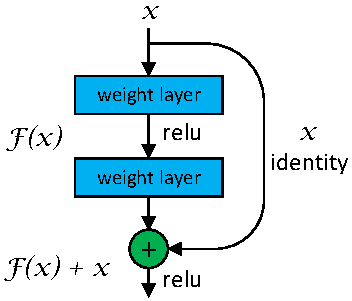
\includegraphics[width=0.77\textwidth]{obrazky-figures/resnetBlock.pdf}
	\caption{Architektura reziduálního bloku s~dvěma vrstvami, kde $F(x)$ je trénovatelné reziduální mapování a~$x$ jsou vstupní data. Převzato z~článku~\cite{website:ResNetIntro}.}
	\label{img:ResNetBlock}
\endminipage\hfill
\minipage{0.48\textwidth}
	\centering
	\setlength{\fboxsep}{0pt}
	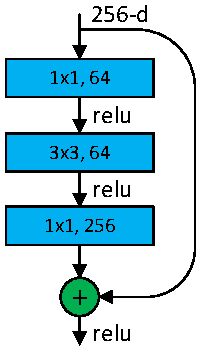
\includegraphics[width=0.41\textwidth]{obrazky-figures/bottleneckBlock.pdf}
	\caption{Architektura bottleneck bloku s~třemi vrstvami použité v~ResNet-50/101/152. Převzato z~článku~\cite{article:DeepResNetForImg}.}
	\label{img:ResNetBottleNeck}
\endminipage\hfill
\end{figure}

ResNet\footnote{ResNet: \url{https://github.com/tensorflow/tpu/tree/master/models/official/resnet}} je rodina reziduálních sítí jako jsou ResNet-18, ResNet-34, ResNet-101~atd., kde číslo na konci udává hloubku sítě. Významnou backbone architekturou~\cite{article:DeepResNetForImg} je \textbf{ResNet-50}, která obsahuje tzv.~bottleneck bloky (viz~obrázek~\ref{img:ResNetBottleNeck}). Bottleneck blok využívá 3 konvoluční vrstvy, kde vrstvy s~rozměry $1 \times 1$ jsou pouze zodpovědné za zmenšení a~následné zvětšení (obnovení) velikosti dat. V~tomto bloku se používá jako zkratka mapování identity, což má za následek snížení času potřebného k~natrénování, avšak přesnost sítě zůstává podobná. ResNet-50 je vylepšený model ResNet-34, který nahrazuje 2-vrstvé bloky za 3-vrstvé a~zvyšuje tím tak svoji hloubku.

\subsubsection{EfficientNet}
EfficientNet\footnote{EfficientNet: \url{https://github.com/tensorflow/tpu/tree/master/models/official/efficientnet}}~\cite{website:RethinkingEfficientNet} je rodina sítí jenž se snaží zlepšit přesnost a~efektivitu modelu pomocí škálování. Existují celkem tři škálovatelné parametry modelu KNN: hloubka, šířka a~rozlišení (viz~obrázek~\ref{img:EfficientNetScaling}). Hloubka, jak již bylo dříve zmíněno, je dána počtem použitých vrstev, zatímco šířka sítě může být definována např.~počtem kanálů v~konvoluční vrstvě. Rozlišení pak jednoduše udává rozlišení vstupního obrazu, který je přiveden na vstup sítě. 

\begin{figure}[hbt]
	\centering
	\setlength{\fboxsep}{0pt}
	\includegraphics[width=1.0\textwidth]{obrazky-figures/EfficientNetScaling.PNG}
	\caption{Škálování modelu KNN. a) je příklad základního modelu, b)-d) je konvenční škálování, které zvětšuje pouze jedenu dimenzi sítě, e) je model vytvořený pomocí složeného škálování, který jednotně škáluje všechny dimenze pevně daným poměrem. Převzato z~článku~\cite{article:RethinkingEfficientNet}.}
	\label{img:EfficientNetScaling}
\end{figure}

\textbf{Škálování hloubky}~\cite{article:RethinkingEfficientNet} je nejběžnější způsob, jak dosáhnout lepší přesnosti. Například ResNet může být škálován od ResNet-18 přidáváním více vrstev až po ResNet-200. Ovšem kvůli běžnému problému s~mizejícím gradientem~aj. nelze zacházet neustále hlouběji. Pokud~\cite{website:RethinkingEfficientNet} je záměrem udržet model malý a~vyhnout se tak problémům provázející hluboké sítě, tak se běžně využívá \textbf{škálování do šířky}, kde širší sítě jsou schopny zachytit i~méně výrazné vzory a~jsou také lépe trénovatelné. Bohužel i~sebevětší šířka neposkytne uspokojující výsledky, jelikož takové modely i~když jsou velmi dobré k~naučení a~následnému zapamatování, tak nejsou schopny generalizace \emph{(overfitting)}, kdežto hlubší modely díky svým vrstvám tak poskytují abstrakci na více úrovních. Pro \textbf{škálování rozlišení} platí, že s~vyšším rozlišením vstupního obrázku je teoreticky možné zachytit více jemných vzorů. Přirozeně tento přístup ale nefunguje lineárně a~zisk přesnosti se po chvíli začne velmi rychle snižovat např.~při zvednutí rozlišení z~$500 \times 500$ na $560 \times 560$ nepřinese takový rozdíl jako z~$220 \times 220$ na $280 \times 280$. Běžně používané rozlišení začíná na $224 \times 224$ a~mezi vysoké rozlišení patří např.~$600 \times 600$. Nejčastěji se však využívá rozlišení $300 \times 300$.

Zvyšování~\cite{website:RethinkingEfficientNet, article:RethinkingEfficientNet} jakéhokoliv rozměru sice zlepšuje přesnost, ale u~větších modelů pak dochází k~saturaci (viz~obrázek~\ref{img:EfficientNetSaturation}). V~praxi je proto nutné škálovat ve všech dimenzích současně a~najít tak mezi nimi rovnováhu. Existuje mnoho postupů, které poskytují obecný návod, jakým způsobem toto škálování provádět, ovšem každý model vyžaduje jiný přístup, a~tak je zapotřebí tuto činnost provádět manuálně. Škálování však nemění operace vrstev, takže k~zajištění vysoké přesnosti je především důležité mít dobrý základní model sítě \emph{(baseline)}, na kterém následně toto škálování provádět. EfficientNet nabízí základní optimalizovaný model pro klasifikaci EfficientNet-B0 a~metodu k~jeho jednotnému škálování pomocí složeného koeficientu. Ostatní modely Efficient-B1 až B7 jsou pak získané jeho dalším škálováním.

\begin{figure}[hbt]
	\centering
	\setlength{\fboxsep}{0pt}
	\includegraphics[width=1.0\textwidth]{obrazky-figures/EfficientNetSaturation.PNG}
	\caption{Škálování baseline modelu různými koeficienty. Z~naměřených hodnot ve všech parametrech je znatelný z~počátku velký nárůst přesnosti sítě, který při vyšších hodnotách začíná saturovat dosáhnutím svých limitů, zatímco nároky na výpočetní výkon déle rostou. Převzato z~článku~\cite{article:RethinkingEfficientNet}.}
	\label{img:EfficientNetSaturation}
\end{figure}

\subsection{Detektory}
\label{sec:Detektory}
Úlohou detektorů~\cite{article:StageDetectors} je predikovat objekt v~obraze a~zároveň ho klasifikovat. Existují dva hlavní typy \emph{state-of-the-art} detektorů, prvním jsou dvoustupňové \emph{(two-stage)}, které v~první fázi používají metody ke zjištění oblastí zájmu a~následně v~druhé fázi tyto oblasti zasílají skrz \emph{\uv{pipeline}} ke klasifikaci a~regresi bounding boxů. Tento typ modelů disponuje vyšší přesností, za cenu delší doby zpracování. Druhým typem jsou jednostupňové \emph{(one-stage)} detektory, které naopak k~detekci přistupují jako k~jednoduchému problému regrese tím, že se ze vstupního obrazu naučí pravděpodobnosti všech tříd a~souřadnic bounding boxů. Tyto modely tak dosahují nižší přesnosti, ale jsou mnohem rychlejší a~umožňují provádět detekci v~reálném čase, jako je např.~SSD\footnote{SSD: \url{https://github.com/amdegroot/ssd.pytorch}}, RetinaNet\footnote{RetinaNet: \url{https://github.com/fizyr/keras-retinanet}}, EfficientDet\footnote{EfficientDet: \url{https://github.com/xuannianz/EfficientDet}}~aj.

\subsubsection{Regionální konvoluční neuronové sítě}
Regionální konvoluční sítě (RCNN) je soubor \emph{two-stage} modelů pro detekci a~klasifikaci v~obraze, jejichž úkolem je dané objekty v~obraze lokalizovat pomocí bounding boxů a~přiřadit je do odpovídajících tříd. Jako první v~této skupině vznikla stejnojmenná architektura \textbf{RCNN}\footnote{RCNN: \url{https://github.com/rbgirshick/rcnn}}~\cite{article:RCNN}, která proces detekce dělí na tři hlavní navazující kroky (viz~obrázek~\ref{img:RCNN}):
\begin{enumerate}
    \item \textbf{Generování oblastí zájmu}~--~V~prvním kroku jsou v~obraze extrahovány kandidátní regiony, které mohou obsahovat hledané objekty. Běžně se jich může vyskytovat 2000 a~více. Pro tento účel se používají algoritmy jako \emph{Selective Search}, \emph{Edge Boxes}~aj.
    \item \textbf{Extrakce příznaků}~--~V~tomto kroku je z~každého regionu extrahován vektor příznaků, který má následně velký podíl pro správnou predikci objektu. RCNN v~tomto kroku používá KNN, i~když dříve se k~tomu účelu využívali algoritmy jako HOG~aj.
    \item \textbf{Klasifikace}~--~V~poslední části je každý region klasifikován podle jeho vektoru příznaků. K~tomu se zde využívají SVM \emph{(Support Vector Machines)} klasifikátory, kde na každou třídu je naučen jeden klasifikátor. Cílem je tak určit predikci na přítomnost objektu v~daném regionu.
\end{enumerate}

\begin{figure}[hbt]
	\centering
	\setlength{\fboxsep}{0pt}
	\includegraphics[width=1.0\textwidth]{obrazky-figures/RCNNmodel.PNG}
	\caption{Schéma architektury RCNN, kde ze vstupního obrázku (1) je jsou extrahovány regiony (2), ze kterých jsou vypočteny vektory příznaků použitím KNN (3). Získané vektory jsou následně použity ke klasifikaci pomocí SVM klasifikátorů (4). Převzato z~článku~\cite{article:RCNN}.}
	\label{img:RCNN}
\end{figure}

Model RCNN~\cite{website:RCNNmodels} však obsahuje několik problému, které mohou znemožňovat jeho nasazení v~praxi. Jedním z~problémů je klasifikace velkého počtu navrhovaných regionů, které znatelně prodlužují čas sítě potřebný pro zpracování obrazu a~jejího natrénování. Navíc v~mnoha případech se regiony překrývají a~dochází tak k~opakovaným výpočtům. Další nevýhodu přináší samotné pevné algoritmy pro extrakci regionů jako \emph{Selective Search}, jelikož v~této fázi neprobíhá žádné učení, a~tato fáze může tedy vest ke generování nevhodných kandidátů. Řešení těchto nedostatků poskytla pak nová architektura Fast-RCNN.

Architektura \textbf{Fast-RCNN}\footnote{Fast-RCNN: \url{https://github.com/rbgirshick/fast-rcnn}}~\cite{website:RCNNmodels, article:FastRCNN} poskytuje podobný přístup jako předešlá architektura RCNN, ale nabízí podstatně větší rychlost a~snižuje její nároky. Tato architektura taktéž z~obrázku generuje kandidátní regiony, avšak je již postupně nepředává do KNN, ale místo toho je ji předána celá množina regionů spolu se vstupním obrázkem, ze kterého je poté vygenerována mapa příznaků (viz~obrázek~\ref{img:FastRCNN}). V~tomto důsledku již nedochází k~redundantním výpočtům a~každá část obrázku je tak zpracována KNN pouze jednou. Následně jsou identifikovány regiony, pomocí region of interest (RoI) pooling vrstvy, která každý kandidátní region převede do mapy příznaků s~pevnou velikostí. Následně jsou mapy regionů převedeny na vektory pomocí sekvence plně propojených vrstev. Výstup sítě je produkován dvěma oddělenými vrstvami, kde softmax vrstva predikuje vektor pravděpodobností tříd daného regionu a~regresní vrstvou, která ve vektoru definuje koordináty příslušného bounding boxu.

\begin{figure}[hbt]
	\centering
	\setlength{\fboxsep}{0pt}
	\includegraphics[width=0.75\textwidth]{obrazky-figures/FastRCNNmodel.PNG}
	\caption{Schéma architektury Fast-RCNN, kde vstupní obrázek a~regiony zájmu (RoI) jsou přivedeny na vstup KNN. Každý RoI je sdružen do mapy příznaků s~pevnou velikostí a~poté převeden na vektor pomocí plně propojených vrstev. Výstupní vrstvy sítě produkují vektor pravděpodobností (softmax) a~vektor offsetů bounding boxu (regressor). Převzato z~článku~\cite{article:FastRCNN}.}
	\label{img:FastRCNN}
\end{figure}

Poslední z~rodiny RCNN je architektura \textbf{Faster-RCNN}\footnote{Faster-RCNN: \url{https://github.com/rbgirshick/py-faster-rcnn}}, která opět vylepšuje svého předchůdce. Architektura Fast-RCNN disponovala nepříliš efektivní metodou generování kandidátních regionů pomocí pevných algoritmů, a~tato část tak tvořila \uv{úzké hrdlo} celého systému, což ovlivňovalo její výkon. Tvůrci tedy přišli s~novým způsobem, který nahrazuje ten starý a~umožňuje síti se tyto kandidátní regiony naučit.

\begin{figure}[H]
	\centering
	\setlength{\fboxsep}{0pt}
	\includegraphics[width=0.5\textwidth]{obrazky-figures/FasterRCNNmodel.PNG}
	\caption{Architektura Faster-RCNN, kde pomocí KNN je ze vstupního obrázku získána mapa příznaků, která slouží jako vstup do RPN a~RoI pooling vrstvy. RPN z~mapy extrahuje kandidátní regiony a~také je předá RoI vrstvě, která díky nim a~disponující mapě příznaků data dále zpracuje, jak je to typické v~architektuře Fast-RCNN. Převzato z~článku~\cite{article:FasterRCNN}.}
	\label{img:FasterRCNNmodel}
\end{figure}

Faster-RCNN~\cite{website:FasterRCNN, article:FasterRCNN} lze rozdělit na dvě části, kde první část je hluboká konvoluční síť tzv.~Region Proposal Network (RPN), která je zodpovědná za generování kandidátních regionů a~druhá část je klasický Fast-RCNN detektor, jenž tyto regiony využívá. Tento přístup nejen zkracuje dobu návrhu regionů z~2~sekund na 10~ms na snímek, ale také umožňuje během této fáze sdílet konvoluční vrstvy s~fázemi detekce z~Fast-RCNN, což celkově zlepšuje predikci příznaků. 

Celý proces~\cite{website:FasterRCNN, article:FasterRCNN} začíná vstupním obrázkem přivedeným do KNN \emph{(backbone)}, který z~něj získá mapu příznaků, jak je znázorněno na obrázku~\ref{img:FasterRCNNmodel}.
Mapa slouží jako vstup do RPN (viz~obrázek~\ref{img:RPN}), která nad ní provádí konvoluci pomocí malého $n \times n$ okna (typicky $3 \times 3$), kde pro každou pozici okna je predikováno několik kandidátních regionů. Regiony jsou reprezentovány \emph{k} kotvami \emph{(anchors)}, přičemž tyto kotvy nejsou finální a~budou dále filtrovány podle jejich \emph{skóre}. Každá kotva má různou velikost a~poměr stran, díky těmto kombinacím je možné detekovat objekty v~různých velikostech a~přesto zachovat okno i~vstupní obrázek v~jednom měřítku. Každá oblast okna je tak s~kandidátními regiony namapována do vektoru příznaků, který je dále poslán do dvou oddělených plně propojených vrstev pro klasifikaci (cls) a~regresi (reg). Klasifikační vrstva udává pouze pravděpodobnost s~jakou se v~daném okně vyskytuje hledaný objekt pomocí \emph{objectness skóre} bez toho, aniž by prováděla jeho klasifikaci do tříd. Regresní vrstva zase určuje regresní koeficienty, které se používají pro určení bounding boxu daného regionu. Získané regiony jsou pak předány spolu se vstupním obrázkem do RoI pooling vrstvy a~následně zpracovány stejným způsobem jako v~architektuře Fast-RCNN.

\begin{figure}[H]
	\centering
	\setlength{\fboxsep}{0pt}
	\includegraphics[width=0.7\textwidth]{obrazky-figures/FasterRCNN_RPN.PNG}
	\caption{Způsob zpracování mapy příznaků v~RPN. Převzato z~článku~\cite{article:FasterRCNN}.}
	\label{img:RPN}
\end{figure}

\subsubsection{You Only Look Once}
\label{sec:YOLO}
You Only Look Once\footnote{YOLO: \url{https://pjreddie.com/darknet/yolo}} (YOLO) je one-stage algoritmus založený na regresi, který namísto hledání oblastí zájmu přímo predikuje třídy a~jejich bounding boxy v~jednom běhu a~umožňuje tak provádět detekci v~reálném čase. Existuje~\cite{website:IntroToYOLO} více variant tohoto algoritmu, ovšem nejčastěji se lze setkat s~verzí YOLOv3.

Algoritmus~\cite{website:IntroToYOLO, article:YOLO} pracuje tak, že nejdříve vstupní obrázek rozdělí do pravidelné mřížky o~velikosti $S \times S$, za účelem najít objekty, které se zde nachází (viz~obrázek~\ref{img:YOLO}). Pokud se střed objektu bude nacházet uvnitř některé buňky v~mřížce, bude tato buňka zodpovědná za jeho detekci. Každá buňka pak predikuje $B$ bounding boxů a~jejich odpovídající \emph{confidence skóre}. Každý box je tak reprezentován pěticí $(x, y, w, h, cs)$, kde $(x, y)$ jsou souřadnice středu boxu, šířka $w$ a~výška $h$ jsou predikované rozměry a~$cs$ je přiřazené skóre. Confidence skóre reflektuje, jak moc si je model jistý, že daný box obsahuje objekt a~také jak moc si myslí, že je přesné jeho ohraničení. Pokud se v~dané oblasti žádný objekt nenachází, mělo by toto skóre být nulové. V~opačném případě je skóre rovno hodnotě tzv.~průniku nad sjednocením \emph{(intersection over union)}, což je technika, která vyjadřuje jak moc se predikované a~reálné boxy překrývají. Tedy v~případě hodnoty 1 je predikovaný box stejný jako ten skutečný a~díky tomu pak lze eliminovat nepřesné rámečky např.~pomocí techniky Non-Maximum Suppression. Kromě toho každá buňka mřížky také predikuje množinu $C$ pravděpodobností pro přiřazení do konkrétních tříd. Tyto pravděpodobnosti jsou predikované na danou buňku, bez ohledu na počet bounding boxů $B$. Výsledné predikce jsou nakonec zakódované v~tenzoru o~velikosti~$S \times S \times (B \cdot 5 + C)$.

\begin{figure}[hbt]
	\centering
	\setlength{\fboxsep}{0pt}
	\includegraphics[width=0.8\textwidth]{obrazky-figures/YOLO_model.PNG}
	\caption{Model YOLO, kde v~tomto případě je vstupní obrázek rozdělen do pravidelné mřížky $7 \times 7$. Každá buňka mřížky predikuje $B$ bounding boxů, jejich odpovídající \emph{confidence skóre} a~$C$ třídních pravděpodobností. Vpravo lze nakonec vidět výsledné predikce. Převzato z~článku~\cite{article:YOLO}.}
	\label{img:YOLO}
\end{figure}

\section{Detekce obličeje}
\label{sec:DetekceObličeje}
První krok pro zpracování obličeje je jeho lokalizace. V~této situaci existuje více metod, které je zde možné využít. Jedním z~přístupů je využití expertních znalostí, kde se využívají charakteristiky lidského obličeje jako je jeho kompozice či barvy. Dalším a~velmi častým přístupem je použití neuronových sítí a~přistupovat k~tomuto problému jako k~detekci objektů. Tyto přístupy také lze kombinovat. Stěžejní vliv na detekci má fakt, že obličeje jsou obecně nasnímány v~různých pozicích, úhlech, výrazu či prostředí a~světelných podmínkách. Aplikaci detekčních algoritmů proto běžně předchází fáze předzpracování, která zahrnuje transformaci barev, filtraci, převzorkování~aj. za účelem zvýšení účinnosti detekce.

\subsection{Viola-Jones algoritmus}
Viola-Jones~\cite{website:FaceDetectionViolaJones} je framework pro detekci objektů publikovaný v~roce 2001 a~ačkoliv se jedná spíše o~zastaralou metodu, tak vykazuje pozoruhodné výsledky při detekci obličejů. Rámec umožňuje také zpracování v~reálném čase, přestože je velmi pomalý na natrénování. Algoritmus pracuje tak, že nejdříve vstupní obraz konvertuje do šedotónového odstínu, protože pak obsahuje méně dat ke zpracování a~lze tak s~ním lépe pracovat. Obličej se na obrázku hledá v~klouzavém okénku, které se postupně posunuje po obrázku, kde velikost okénka a~posunu lze libovolně nastavit. Ovšem menšími posuny je možné dosáhnout větší přesnosti lokalizace. Algoritmus při zpracování obsahuje čtyři hlavní kroky:

\begin{enumerate}
    \item Detekce Haarových příznaků
    \item Vytvoření integrálního obrazu
    \item Spuštění tréninku AdaBoost
    \item Sestavení kaskády klasifikátorů
\end{enumerate}

Pro detekci příznaků~\cite{website:FaceDetectionViolaJones, website:FacialRecognitionViolaJones} se v~klouzavém okénku používají celkem tři typy \textbf{Haarových příznaků} (viz~obrázek~\ref{img:HaarLikeFeatures}), které jsou převzaty z~konceptu Haarových vlnek. Tyto příznaky představují funkce se světlou a~tmavou oblastí, které se používají pro detekci rysů. Výsledek je prezentován jedinou hodnotou jako součet hodnot intenzit pixelů v~tmavé oblasti mínus součet intenzit pixelů ve světlé oblasti. Hodnota bude nulová v~případě, kdy všechny pixely mají stejnou hodnotu a~oblast tak nenese žádnou informaci. Na obličeji se ve skutečnosti vyskytují velmi rozdílné oblasti, které poskytnou vysokou hodnotu. Takový přechod z~tmavé oblasti do světlé může definovat okraj obočí, či lesklá linie mezi tmavými oblastmi může indikovat nos. Aplikací všech funkcí na různé pozice může nakonec určit zda obraz obsahuje lidskou tvář či nikoliv.

\begin{figure}[hbt]
	\centering
	\setlength{\fboxsep}{0pt}
	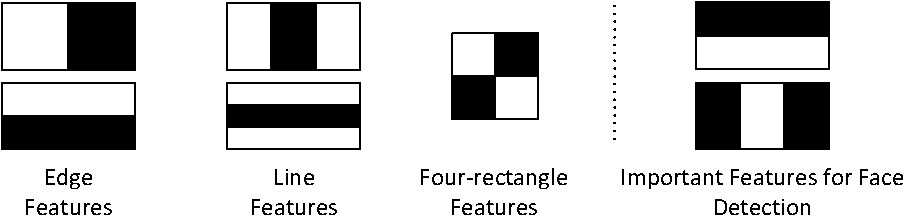
\includegraphics[width=0.9\textwidth]{obrazky-figures/haar_features.pdf}
	\caption{Haarovi příznaky pro detekci hran, linií a~čtyřstranného příznaku. Převzato z~článku~\cite{website:FacialRecognitionViolaJones}.}
	\label{img:HaarLikeFeatures}
\end{figure}

Ve skutečnosti~\cite{website:FaceDetectionViolaJones, website:FacialRecognitionViolaJones} výpočet hodnoty může být velmi náročný v~případě rozlehlého příznaku, který zahrnuje velké množství pixelů. V~tomto případě se používá technika \textbf{integrálního obrazu}, která dovoluje tyto výpočty provádět snadno a~efektivně, čímž umožní rychle rozpoznat, zda příznak odpovídá jeho kritériím. Výpočet integrálního obrazu je realizován tak, že hodnota konkrétního pixelu je dána součtem všech pixelů v~oblasti od jeho pozice k~levému hornímu rohu, jak je znázorněno na obrázku~\ref{img:IntegralImageCreation}. Výčet pak výsledné hodnoty z~oblasti lze realizovat pouze pomocí čtyř hodnot z~integrálního obrazu podle následujícího vzorce~\ref{eqn:IntegralImage} s~referencí na obrázek~\ref{img:IntegralImageCalculation}.

\begin{equation}
    \label{eqn:IntegralImage}
    oblast = I(D) + I(A) - I(B) - I(C),
\end{equation}
kde $I(D)$ je hodnota intenzity pixelu v~integrálním obraze uvnitř oblasti v~pravém dolním rohu, $I(A)$ je hodnota mimo oblast v~levém horním rohu, $I(B)$ a~$I(C)$ jsou hodnoty pixelů mimo oblast v~pravém horním a~levém dolním rohu.

\begin{figure}[hbt]
\minipage{0.48\textwidth}
	\centering
	\setlength{\fboxsep}{0pt}
	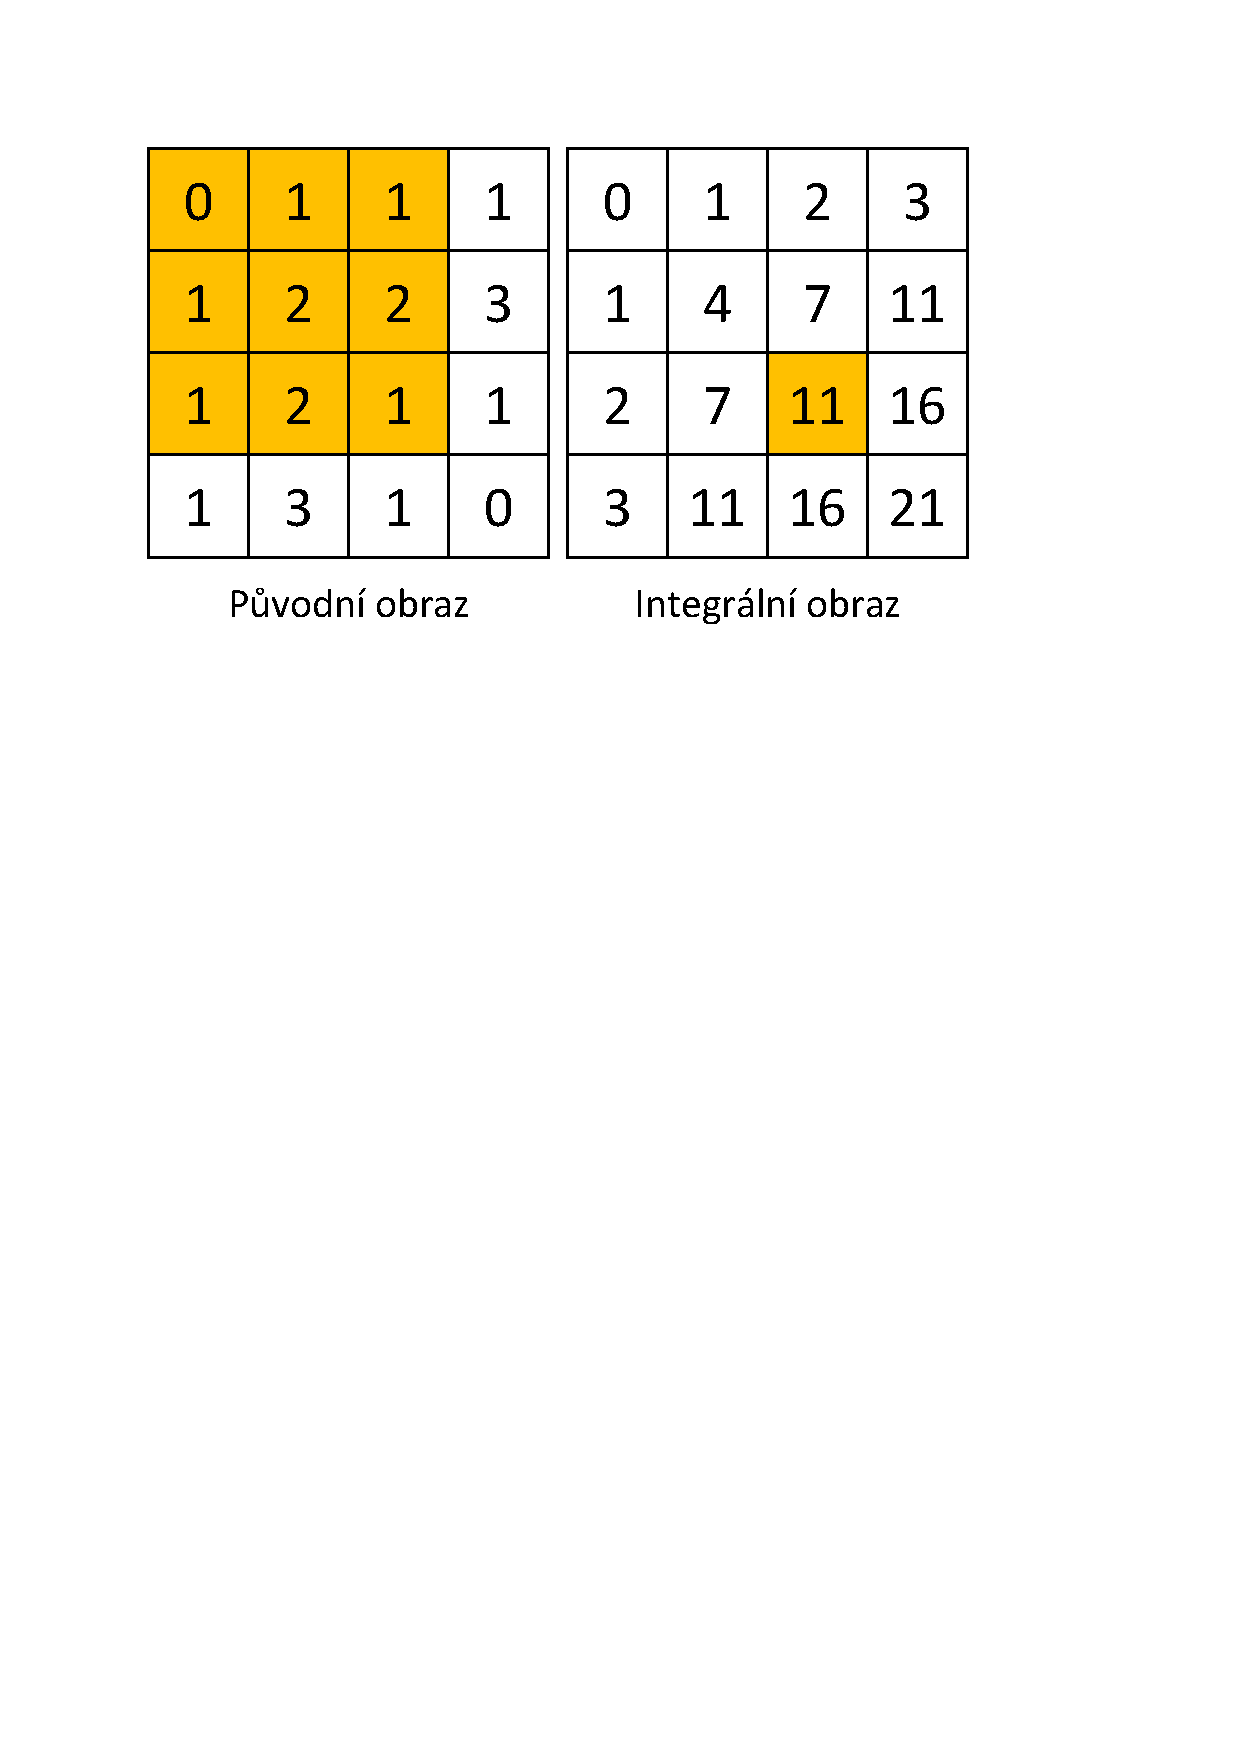
\includegraphics[width=1.0\textwidth]{obrazky-figures/IntegralImageCreation.pdf}
	\caption{Ukázka výpočtu pixelu v~integrálním obraze, jehož hodnota je dána součtem pixelů z~původního obrazu z~oblasti od jeho aktuálního umístění směrem k~levému hornímu rohu. Převzato z~článku~\cite{website:FaceDetectionViolaJones}.}
	\label{img:IntegralImageCreation}
\endminipage\hfill
\minipage{0.48\textwidth}
	\centering
	\setlength{\fboxsep}{0pt}
	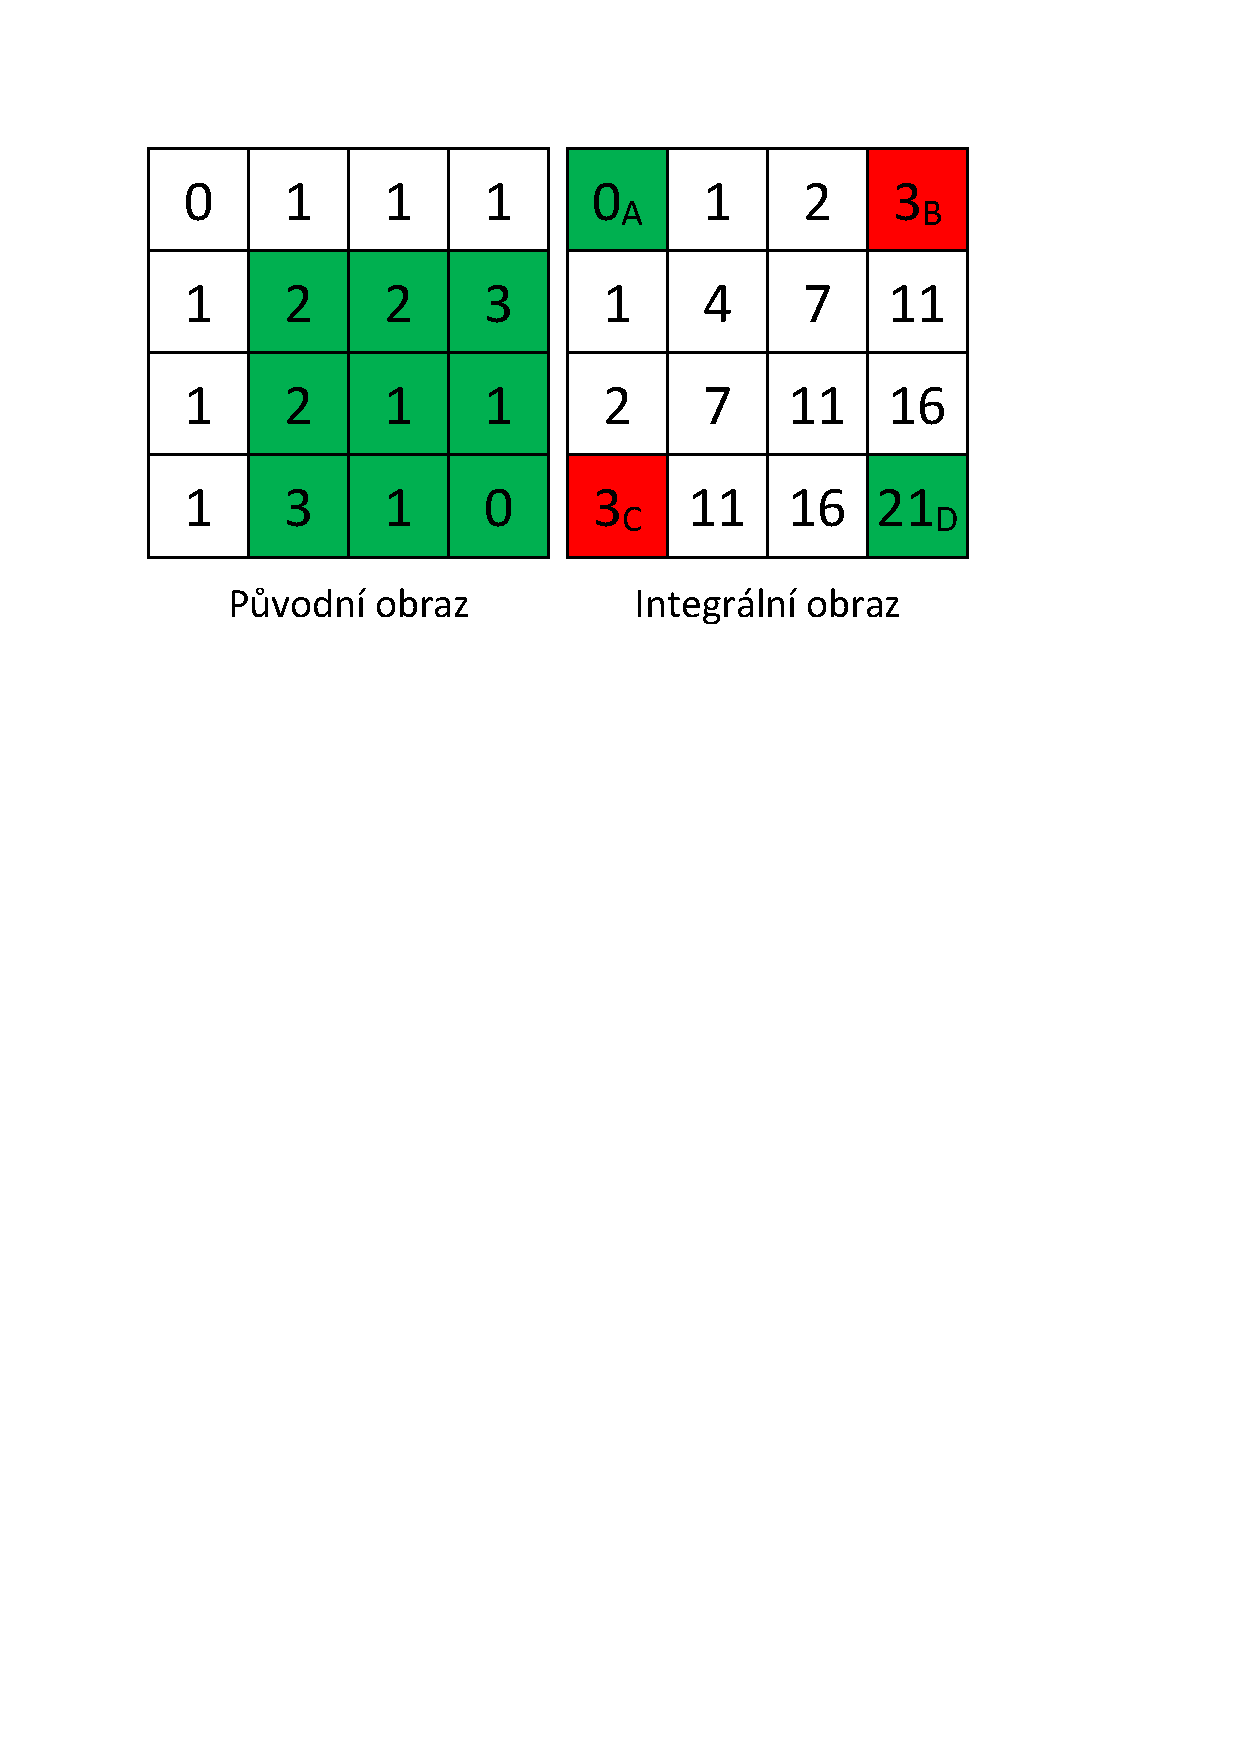
\includegraphics[width=1.0\textwidth]{obrazky-figures/IntegralImageCalculation.pdf}
	\caption{Výpočet hodnoty oblasti z~integrálního obrazu podle vzorce~\ref{eqn:IntegralImage}, kde \newline $21 + 0 - 3 - 3 = 15$, je to stejné jako $2 + 2 + 3 + 2 + 1 + 1 + 3 + 1 + 0 = 15$. Převzato z~článku~\cite{website:FaceDetectionViolaJones}.}
	\label{img:IntegralImageCalculation}
\endminipage\hfill
\end{figure}

Jako další krok~\cite{website:FaceDetectionViolaJones} v~rámci Viola-Jones se používá algoritmus strojového učení pro zlepšení výkonnosti známý jako \textbf{AdaBoost} \emph{(Adaptive Boosting)}. Pokud bude použita velikost detekčního okénka $24 \times 24$, tak počet přítomných příznaků potom může dosahovat až~$160 000$, kdežto jen pár z~nich je pro detekci obličeje opravdu důležitých. AdaBoost proto \emph{rozhoduje} o~tom, jaké typy a~velikosti Haarových příznaků budou součástí výsledného klasifikátoru. Jinak řečeno každý Haarův příznak reprezentuje slabý klasifikátor a~AdaBoost pomocí těchto slabých klasifikátorů má za úkol sestavit jeden silný klasifikátor. Vyhodnocení výkonnosti každého klasifikátoru se provádí na označených datech pro trénování. Po vyhodnocení se vyberou klasifikátory, které vykazovaly nejvyšší odezvu nad obrázky s~tvářemi, zatímco obrázky bez tváří vyhodnocovaly negativně. Těmto klasifikátorům se přiřadí váhy podle jejich výkonnosti a~budou nakonec součástí silného klasifikátoru.

Přestože AdaBoost~\cite{website:FaceDetectionViolaJones, website:FacialRecognitionViolaJones} výrazně napomáhá výběru relevantních příznaků, stále obsahuje mnoho výpočtů na to, aby byly všechny aplikovány v~každé pozici okna. K~tomuto účelu se využívá \textbf{kaskáda klasifikátorů}, která zvyšuje rychlost tím, že se snaží, co nejrychleji zahodit výpočet nad snímky bez tváře. Proces probíhá tak, že nad oknem je použit nejlepší disponující silný klasifikátor (např.~identifikace hřbetu nosu), který rozhodne o~přítomnosti příznaku. Pokud příznak v~okně není dostupný, tak je okno zahozeno a~již není dále zpracováno. V~případě, kdy bude příznak detekován, tak bude zpracován druhým nejlepším klasifikátorem, který má opět možnost celé okno zahodit. Postupně je takto zpracována celá kaskáda vybraných klasifikátorů a~pokud se dané okno dostane až na její konec, znamená to, že všechny klasifikátory potvrdily shodu a~na snímku je detekován obličej.

\subsection{Histogram orientovaných gradientů}
Histogram orientovaných gradientů (HOG) je algoritmus pro detekci objektů, který se dá aplikovat i~na lidský obličej. V~prvním kroku~\cite{website:IntroToHOG} algoritmu jsou vypočteny hodnoty gradientů pro každý pixel ve vstupním obraze, jenž udávají změnu intenzity na osách $x$ a~$y$. Ve směru $x$ se gradient vypočítá odečtením hodnoty intenzity levého souseda od hodnoty intenzity pravého souseda. Gradient ve směru $y$ odečtením intenzity horního pixelu od hodnoty spodního pixelu. Hodnota vyjde vysoká v~případě, kdy dojde k~velkému rozdílu intenzit (např.~na okrajích objektů). Pro tento výpočet se používají 1D masky, které jsou znázorněny v~definici~\ref{eqn:HOGMask}.

\begin{equation}
    \label{eqn:HOGMask}
    g_x = 
    \begin{bmatrix}
        -1 & 0 & 1
    \end{bmatrix}
    \qquad
    g_y = 
    \begin{bmatrix}
        -1 \\
        0 \\
        1
    \end{bmatrix}
\end{equation}

Dalším krokem~\cite{website:IntroToHOG} je určení velikosti a~směru výsledného gradientu pro každý pixel. Velikost gradientu se spočítá pomocí Pythagorovy věty a~jeho úhel pomocí funkce arctan, viz~následující vzorce~\ref{eqn:HOGGradient}.

\begin{equation}
    \label{eqn:HOGGradient}
    g = \sqrt{g_{x}^{2} + g_{y}^{2}}
    \qquad
    \phi = arctan \left( \frac{g_y}{g_x} \right)
\end{equation}

Potom~\cite{website:IntroToHOG} co je pro každý pixel spočítán jeho gradient, je obrázek rozdělen do pravidelné mřížky. Běžně se využívá velikost buňky $8 \times 8$ pixelů, ale obecně lze zvolit libovolnou velikost~--~záleží na úrovni detailu. V~každé buňce mřížky se spočítá histogram gradientů, který definují odpovídající pixely. Histogram představuje vektor o~velikosti devíti tříd, jenž definuje rozsahy orientací gradientů s~rozmezím $20$\textdegree\space (od $0$\textdegree\space do $180$\textdegree\space při použití znaménka). Každý pixel tak může přispět do dvou tříd, kde celková velikost příspěvku je dána velikostí jeho gradientu. Třídy do kterých přispěje, ohraničují interval jeho spočtené orientace gradientu a~konkrétní přidaná velikost do dané třídy je dána poměrově. Tedy vyšší příspěvek bude ve třídě, která má hodnotu bližší jeho orientaci.

Nyní je obrázek rozdělen na menší úseky v~mřížce a~pro každý úsek je spočítán histogram orientací gradientů. Protože jsou gradienty citlivé na osvětlení a~některé části obrázku jsou světlejší než jiné, tak se provádí normalizace osvětlení, která zvyšuje odolnost příznaku na světelných podmínkách. Normalizace se provádí na čtyřech buňkách (v tomto případě $16 \times 16$ pixelů), kde každá buňka obsahuje vektor (histogram) gradientů o~velikosti $9$, které se spojí do jednoho vektoru s~velikostí $36$. Tento spojený vektor~\cite{article:HOG4Detection} se následně normalizuje pomocí metody L2-norm (lze i~jinak)~--~viz~následující vzorec~\ref{eqn:HOGNorm}.

\begin{equation}
    \label{eqn:HOGNorm}
    f = \frac{v}{\sqrt{||v||_{2}^{2} + e^{2}}},
\end{equation}
kde $v$ je nenormalizovaný vektor obsahující všechny histogramy v~daném bloku, $||v||_{2}$ je jeho 2-norma a~$e$ je malá konstanta. Tato normalizace~\cite{website:IntroToHOG} je provedena pomocí klouzavého okénka přes celý obrázek. Při velikosti obrázku $64 \times 128$ pixelů a~velikosti normalizačního bloku $16 \times 16$ vznikne celkem $7 \cdot 15 = 105$ posunů bloku, kde každý posun generuje vektor příznaků o~velikosti $36$. Výsledný vektor příznaků celého obrázku bude pak mít velikost $105 \cdot 36 = 3780$ prvků, který je nakonec klasifikován pomocí binárního klasifikátoru SVM \emph{(Support Vector Machines)}.

\subsection{Detekce obličeje pomocí neuronových sítí}
Moderní přístupy pro detekci obličeje používají neuronové sítě a~přistupují k~tomuto problému jako k~detekci objektů. Jedním z~důvodů je to, že i přesto, že přístupy jako Viola-Jones dosahují dobrého výkonu v~reálném čase, tak se tyto detektory mohou výrazně zhoršit při aplikaci na lidské tváře s~většími vizuálními variacemi, které se ve skutečném světě nacházejí. V~následující části jsou proto lehce přiblížený některé architektury, na které lze aktuálně v~této oblasti narazit.

\subsubsection{Multi-task Cascaded Convolutional Networks}
Multi-task Cascaded Convolutional Networks\footnote{MTCCN: \url{https://github.com/ipazc/mtcnn}} (MTCNN)~\cite{website:MTCNN} je framework pro detekci a~následné zarovnání obličeje s~lokalizací orientačních bodů. Celý proces funguje v~\emph{\uv{pipeline}}, která je rozdělena do tří fází, kde každá fáze obsahuje konvoluční neuronovou síť. Cílem je ohraničit obličej a~umístit orientační body na jeho oči, nos a~ústa. V~první části se používá mělká síť (P-Net) pro rychlý návrh kandidátních regionů, v~další části se pak tyto regiony upřesní složitější sítí (R-Net) a~v~konečné fázi dojde k~dalšímu zpřesnění a~určení pozic bodů pomocí komplexní KNN (O-Net). Architektury těchto sítí lze vidět na obrázku~\ref{img:MTCNN}.

První krok~\cite{website:MTCNN, article:MTCNN} obsahuje plnou konvoluční síť (FCN, tj. nepoužívá žádnou plně propojenou vrstvu a~je složena pouze z~konvolučních vrstev), která se používá k~získání kandidátních regionů a~regresi jejich bounding boxů. Získané bounding boxy, reprezentovány vektory, jsou následně vyfiltrovány technikou Non-Maximum Suppresion (NMS), která eliminuje překrývající se regiony. V~druhé fázi jsou všechny tyto regiony přivedeny na vstup běžné konvoluční sítě, která dále provede redukci nesprávných oblastí, kalibraci s~regresí bounding boxů a~NMS. Výstupem této vrstvy jsou tři vektory, kde první určuje zda vstup obsahuje obličej, další vektor o~velikosti $4$ definuje rozměry bounding boxu a~vektor s~$10$-ti prvky pro souřadnice orientačních bodů obličeje. Poslední fáze je velmi podobná druhé fázi, ale v~tomto případě jde o~detailnější analýzu obličeje, kde síť vygeneruje pět výsledných orientačních bodů na obličeji.

\begin{figure}[hbt]
	\centering
	\setlength{\fboxsep}{0pt}
	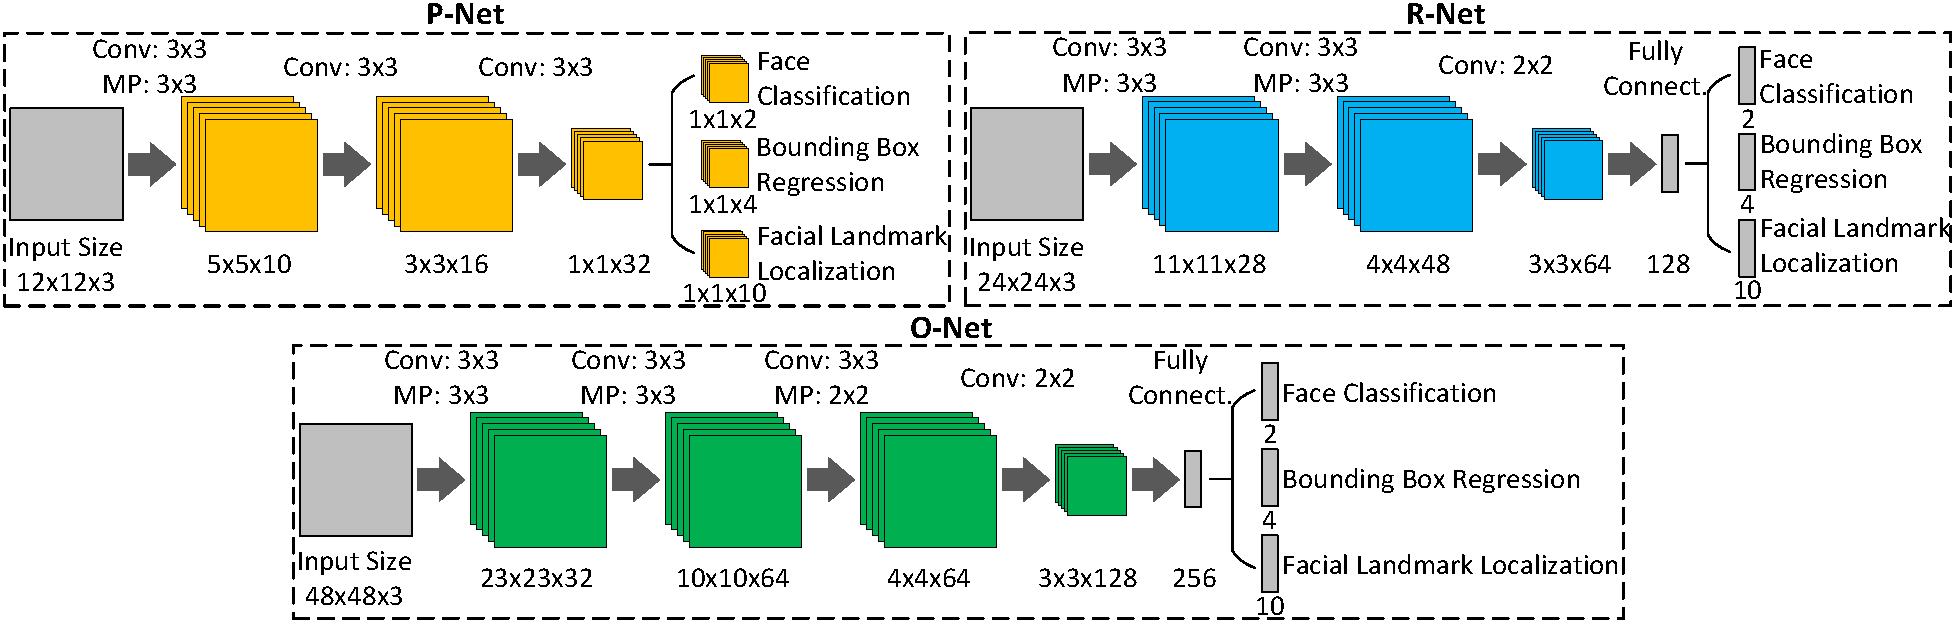
\includegraphics[width=1.0\textwidth]{obrazky-figures/MTCNN.pdf}
	\caption{Architektura sítí P-Net \emph{(Proposal Network)}, R-Net \emph{(Refine
Network)} a~O-Net \emph{(Output Network)}. Velikost kroku v~konvolučních vrstvách je $1$ a~v~pooling vrstvách $2$. Převzato z~článku~\cite{article:MTCNN}.}
	\label{img:MTCNN}
\end{figure}

\subsubsection{RetinaFace}
RetinaFace\footnote{RetinaFace: \url{https://github.com/serengil/retinaface}}~\cite{article:RetinaFace} je jednostupňový detektor obličeje, jenž provádí lokalizaci po pixelech na různých velikostech tváří s~podporou strojového učení. Využívá \emph{multi-task} strategii k~současné predikci skóre obličeje, jeho bounding boxu, 3D rekonstrukci a~odhadu pěti orientačních bodů na obličeji stejně jako v~případě MTCNN.

Architektura řešení~\cite{article:RetinaFace, website:RetinaFace} se skládá z~pyramidy příznaků, z~kontextového modulu a~z~kaskády \emph{multi-task loss} funkcí~--~viz~obrázek~\ref{img:RetinaFaceArchitecture}. Do pyramidy příznaků je přiveden vstupní obrázek, nad kterým je vygenerováno pět různých velikostí. První čtyři mapy příznaků jsou vypočítány pomocí sítě ResNet-152, která byla předtrénována na datasetu ImageNet-11k. Poslední mapa je spočtena pomocí konvoluce $3 \times 3$ s~krokem $2$, kde hodnoty jsou náhodně inicializovány metodou \emph{\uv{Xavier}}. Inspirací SSH\footnote{Single Stage Headless Face Detector: \url{https://github.com/mahyarnajibi/SSH}} a~PyramidBox\footnote{PyramidBox: \url{https://github.com/yxlijun/Pyramidbox.pytorch}} byly i zde aplikovány nezávislé kontextové moduly na úrovně pyramidy za účelem vylepšení modelovaného kontextu. Ovšem všechny $3 \times 3$ konvoluční vrstvy byly nahrazeny deformovatelnou konvoluční sítí (DCN).

\begin{figure}[hbt]
	\centering
	\setlength{\fboxsep}{0pt}
	\includegraphics[width=1.0\textwidth]{obrazky-figures/RetinaFaceArchitecture.PNG}
	\caption{RetinaFace je navržena na pyramidě příznaků s~nezávislými kontextovými moduly. V~návaznosti na kontextové moduly jsou spočítány \emph{multi-task loss} funkce pro každou kotvu. Převzato z~článku~\cite{article:RetinaFace}.}
	\label{img:RetinaFaceArchitecture}
\end{figure}

Ke zlepšení lokalizace obličeje~\cite{website:RetinaFace} je použita kaskádová regrese spolu s~\emph{multi-task loss} funkcí. Tento mechanismus funguje tak, že první kontextový modul predikuje bounding box pomocí běžných kotev a~poté následující moduly předpovídají přesnější boxy pomocí regresních kotev. Ztrátová funkce má následující tvar~\ref{eqn:MultiTaskLoss}.

\begin{equation}
    \label{eqn:MultiTaskLoss}
    L = L_{cls}(p_{i}, p_{i}^{*}) + \lambda_{1} \cdot p_{i}^{*} \cdot L_{box}(t_{i},t_{i}^{*}) + \lambda_{2} \cdot p_{i}^{*} \cdot L_{pts}(l_{i},l_{i}^{*}) + \lambda_{3} \cdot p_{i}^{*} \cdot L_{pixel},
\end{equation}
kde $L_{cls}(p_{i}, p_{i}^{*})$~\cite{article:RetinaFace} reprezentuje klasifikaci obličeje, přičemž $p_{i}$ je predikovaná pravděpodobnost, že kotva $i$ obsahuje obličej a~$p_{i}^{*}$ je $1$ pro pozitivní kotvu a~$0$ pro negativní. $L_{cls}$ je softmax ztrátová funkce pro binární klasifikaci. Regrese bounding boxu je dána $L_{box}(t_{i},t_{i}^{*})$, kde $t_{i}$ a~$t_{i}^{*}$ jsou souřadnice predikovaného a~\emph{ground truth} boxu. Souřadnice jsou normalizovány ve středovém formátu a~$L_{box}(t_{i},t_{i}^{*}) = R(t_{i} - t_{i}^{*})$, kde $R$ je ztrátová funkce $smooth - L_{1}$ definovaná v~\cite{article:FastRCNN}. Regrese pěti bodů na obličeji je $L_{pts}(l_{i},l_{i}^{*})$, kde $l_{i}$ a~$l_{i}^{*}$ reprezentují predikované a~anotované body, $L_{pts}$ je stejná ztrátová funkce jako $R$ při regresi ohraničení. $L_{pixel}$ je hustá regresní funkce popsaná v~\cite{article:RetinaFace}. Parametry pro vyvážení funkce $\lambda_{1} - \lambda_{3}$ jsou nastaveny na $0,25$, $0,1$ a~$0,01$, čímž zvyšují význam ohraničení a~poté bodům na obličeji. Výstup z~této metody lze vidět na obrázku~\ref{img:RetinaFaceMultiTaskLoss}.

\begin{figure}[hbt]
	\centering
	\setlength{\fboxsep}{0pt}
	\includegraphics[width=0.8\textwidth]{obrazky-figures/RetinaFaceMultiTaskLoss.PNG}
	\caption{Každá pozitivní kotva poskytuje skóre obličeje, jeho ohraničení, pět orientačních bodů a~vrcholy 3D obličeje promítnuté na rovinu obrazu. Převzato z~článku~\cite{article:RetinaFace}}
	\label{img:RetinaFaceMultiTaskLoss}
\end{figure}

\section{Rozpoznávání osob podle obličeje}
Rozpoznání obličeje je proces, během kterého je tvář ze vstupního obrázku rozpoznávána vůči databázi již známých tváří. Moderní systémy dělí tento proces na čtyři kroky: detekce, zarovnání, reprezentace a~klasifikace. Detekci obličeje byla věnována předchozí sekce~\ref{sec:DetekceObličeje} a~pro tento účel je možné použít např.~algoritmus Viola-Jones. Opět zde existuje více přístupů, které lze pro identifikaci uplatnit a~dále jsou uvedeny pouze některé představitelé \emph{state-of-the-art}, které v~této oblasti utvořili významné milníky.

\begin{figure}[hbt]
	\centering
	\setlength{\fboxsep}{0pt}
	\includegraphics[width=0.7\textwidth]{obrazky-figures/DeepFaceAlignment.PNG}
	\caption{Proces zarovnání obličeje. (a)~Detekovaný obličej pomocí $6$-ti referenčních bodů. (b)~Zarovnaný a~oříznutý 2D obličej. (c)~Na 2D oříznuté tváři je detekováno $67$~bodů. (d)~Referenční 3D reprezentace obličeje. (e)~Viditelnost trojúhelníku s~ohledem na pozici kamery za účelem odhadu orientace obličeje. (f)~Všech $67$~bodů reprezentovaných 3D modelem je použito k~natočení 2D modelu. (g)~Konečný frontalizovaný výřez obličeje. (h)~Nový pohled generovaný 3D modelem (pro zajímavost). Převzato z~článku~\cite{article:DeepFace}.}
	\label{img:DeepFaceAlignment}
\end{figure}

\subsection{DeepFace}
\label{sec:DeepFace}
DeepFace\footnote{DeepFace: \url{https://github.com/serengil/deepface}} je systém pro rozpoznávání obličejů vytvořený společností Facebook, který ho využívá k~označování osob na obrázku. K~rozpoznávání používá devítivrstvou neuronovou síť, která obsahuje více než $120$ mil. parametrů a~byla natrénována na datasetu se $4$ mil. označených obrázků s~obličeji od uživatelů Facebooku. Autoři uvádějí přesnost modelu na $97,35$~\%, čímž může dosahovat vyšší přesnosti než člověk. Tento model vyniká především vlastním způsobem zarovnání tváře a~reprezentace rysů, které využívá namísto konvenčních metod strojového učení. Tato skutečnost pak umožňuje provést analýzu nad větším množství dat.

Cílem~\cite{website:DeepFace} zarovnání tváře je ze vstupního obrázku, který může obsahovat libovolně pootočený obličej, vygenerovat pohled na jeho čelní stranu. K~tomuto účelu byla navržena metoda 3D frontalizace, během niž dochází k~2D zarovnání, poté 3D zarovnání a~ke konečné frontalizaci (viz~obrázek~\ref{img:DeepFaceAlignment}). Konkrétně~\cite{article:DeepFace} celý proces obsahuje následující kroky:

\begin{enumerate}
    \item \textbf{Detekce referenčních bodů}~--~Ve vstupním obrázku je identifikován obličej pomocí šesti referenčních bodů, kde dva body jsou na očích, jeden na špičce nosu a~tři body na ústech.
    \item \textbf{Zarovnání a~oříznutí}~--~Následně pomocí detekovaných bodů je tvář oříznuta a~vzniká tak 2D obrázek obličeje.
    \item \textbf{Detekce $67$ bodů}~--~Na obrázek obličeje se aplikuje mapa $67$ referenčních bodů za účelem vygenerovat odpovídající 3D model. Tento krok je velmi důležitý pro kompenzaci rotace obličeje.
    \item \textbf{Odhad orientace}~--~Poté je proveden odhad orientace obličeje pomocí vztahu mezi jeho 2D a~3D reprezentací.
    \item \textbf{Zarovnání obličeje}~--~V~poslední fázi je 3D reprezentace transformována do frontálního pohledu. Výsledkem je tvář v~čelním pohledu, která je vizuálně podobná obličeji skutečného jednotlivce.
\end{enumerate}

Potom~\cite{website:DeepFace, article:DeepFace} co je obličej zarovnaný a~reprezentovaný RGB obrázkem o~velikosti $152 \times 152$, následuje proces klasifikace pomocí hluboké neuronové sítě (viz~obrázek~\ref{img:DeepFaceArchitecture}). Síť zpočátku obsahuje konvoluční vrstvu s~$32$ filtry o~velikosti $11 \times 11$ následovanou max-pooling vrstvou $3 \times 3$ s~krokem $2$ a~konvoluční vrstvou 16 filtrů $9 \times 9$. Tyto vrstvy mají za úkol získat nízkoúrovňové příznaky jako jsou hrany a~textury.

Následují~\cite{website:DeepFace, article:DeepFace} další tři lokálně propojené vrstvy, které stejně jako konvoluční vrstvy obsahují sadu filtrů, jenom je každý filtr aplikovaný na jinou oblast v~mapě příznaků. Tím architektura sítě využívá skutečnosti, že různé oblasti v~zarovnaném obrázku mají různou entropii, např.~oblast mezi očima a~obočím vykazuje vysokou míru rozlišitelnosti oproti oblasti mezi ústy a~nosem. Poslední dvě vrstvy jsou plně propojené a~jsou schopny zachytit korelaci mezi prvky obličeje. Výstup předposlední vrstvy reprezentuje obličej jako vektor příznaků a~výstup poslední plně propojené vrstvy je zpracován softmax funkcí, jenž vytváří distribuci mezi třídami. Poslední lokálně a~plně propojené vrstvy obsahují velké množství parametrů (zhruba $95$~\% parametrů sítě).

\begin{figure}[hbt]
	\centering
	\setlength{\fboxsep}{0pt}
	\includegraphics[width=1.0\textwidth]{obrazky-figures/DeepFaceArchitecture.png}
	\caption{Architektura sítě DeepFace. Předzpracovaný obrázek je předán konvoluční vrstvě, která je následovaná pooling a~poté další konvoluční vrstvou. Dále jsou aplikovány tři lokálně propojené vrstvy a~na konci se nachází dvě plně propojené. Převzato z~článku~\cite{article:DeepFace}.}
	\label{img:DeepFaceArchitecture}
\end{figure}

\subsection{FaceNet}
FaceNet\footnote{FaceNet: \url{https://github.com/davidsandberg/facenet}}~\cite{article:FaceNet} je model vytvořený společností Google, který dosahuje velmi vysoké přesnosti na rozsáhlých datasetech jako je $95,12$~\% na databázi obličejů YouTube nebo $99,63$~\% na LFW \emph{(Labeled Faces in the Wild)}. Pracuje tak~\cite{website:FaceNetIntro}, že každý obrázek obličeje mapuje do Euklidovského prostoru, kde vzdálenosti mezi jednotlivými tvářemi odpovídají jejím podobnostem. Jako základní architekturu~\cite{website:FaceNet} využívá ZF-Net nebo Inception, na kterých dále staví. Přidává několik konvolučních vrstev $1 \times 1$ za účelem snížení počtu parametrů a~využívá \emph{end-to-end} učení. Výstupem použité neuronové sítě je vektor příznaků \emph{(embedding)} o~velikosti $128$, na kterém je provedena $L_{2}$ normalizace. Tyto embeddingy jsou pak předány loss funkci, která definuje podobnost obličeje (viz~obrázek~\ref{img:FaceNetArchitecture}). Cílem aplikované loss funkce je zajistit, aby kvadratická vzdálenost mezi dvěma obrázky tváře byla malá v~případě stejné identity osoby a~byla nezávislá na stavu snímku či výrazu jedince. Naopak musí poskytnout velkou odezvu v~případě snímků s~rozdílnými osobami. K~tomuto účelu byla představena nová ztrátová funkce nazývaná Triplet loss.

\begin{figure}[hbt]
	\centering
	\setlength{\fboxsep}{0pt}
	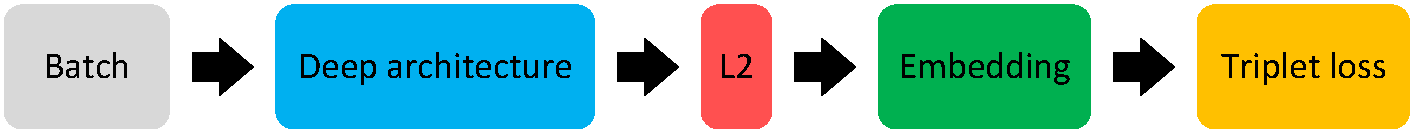
\includegraphics[width=1.0\textwidth]{obrazky-figures/FaceNetArchitecture.pdf}
	\caption{Struktura modelu FaceNet, kde na vstupní vrstvu je přiveden batch a~hluboká KNN je následována $L_{2}$ normalizací, jejíž výsledkem je embedding obličeje, který slouží jako vstup Triplet loss funkce. Převzato z~článku~\cite{article:FaceNet}.}
	\label{img:FaceNetArchitecture}
\end{figure}

\textbf{Triplet loss funkce}~\cite{website:FaceNetIntro} využívá trojici obrázků: referenční \emph{(anchor)}, pozitivní a~negativní. Cílem je, aby vstupní obrázek obličeje $x_{i}^{a}$ \emph{(anchor)} byl blíže pozitivním obrázkům $x_{i}^{p}$, které patří stejné osobě, než těm ostatním $x_{i}^{n}$, jenž obsahují odlišné osoby (viz~obrázek~\ref{img:TripletLossLearning}). Funkci lze formálně definovat vztahem~\ref{eqn:TripletLoss}.

\begin{equation}
    \label{eqn:TripletLoss}
    L = \sum_{i}^{N} \left[ ||f(x_{i}^{a}) - f(x_{i}^{p})||_{2}^{2} - ||f(x_{i}^{a}) - f(x_{i}^{n})||_{2}^{2} + \alpha \right]_{+},
\end{equation}
kde $x_i$ reprezentuje obrázek, $f(x_i)$ jeho odpovídající embedding a~$\alpha$ je hyperparametr, který definuje hranici rozlišitelnosti neboli prahovou hodnotu, která určuje rozdíl mezi páry obrázků.

\begin{figure}[hbt]
	\centering
	\setlength{\fboxsep}{0pt}
	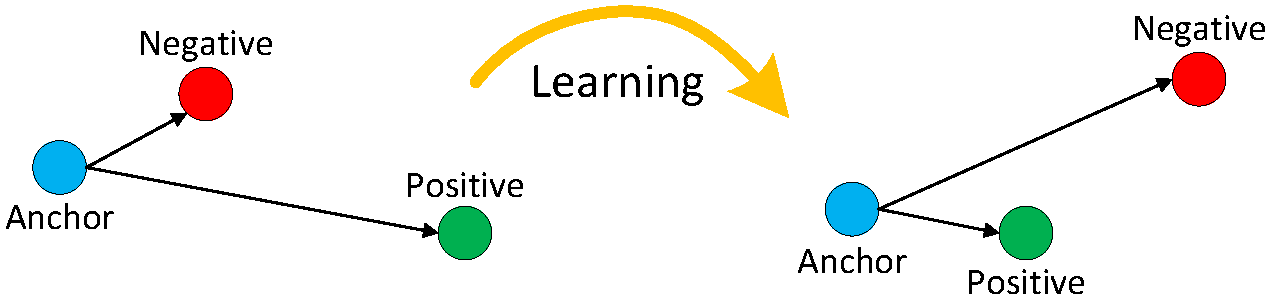
\includegraphics[width=0.9\textwidth]{obrazky-figures/TripletLoss.pdf}
	\caption{Triplet loss funkce se snaží minimalizovat vzdálenost mezi referenčním obrázkem a~jeho pozitivním vzorkem, který spadá do stejné třídy a~přitom maximalizovat vzdálenost od negativních prvků, které obsahují jinou totožnost. Převzato z~článku~\cite{article:FaceNet}.}
	\label{img:TripletLossLearning}
\end{figure}

Výběr správných trojic~\cite{website:FaceNetIntro, website:FaceNet} obrázků je velmi důležitý, protože existuje mnoho párů, které podmínku vzdálenosti splní a~model tak bude při učení velmi pomalu konvergovat. K~rychle konvergenci je proto důležité vybrat takové obrázky, které porušují výše uvedenou rovnici~\ref{eqn:TripletLoss}. Tedy takové, aby vzdálenost mezi referenčním a~pozitivním obrázkem byla co největší a~zároveň vzdálenost mezi referenčním a~negativním případem byla co nejmenší. Potom bude model zpracovávat pouze užitečné informace a~jeho učení se urychlí. Najít takové páry je ovšem výpočetně náročné, a~tak se hledají pouze v~rámci mini-batche (tj.~1000-2000~vzorků).

\section{Sledování objektů}
Sledování objektů \emph{(tracking)}~\cite{article:Tracking} je poměrně častá úloha při zpracování videozáznamu, která umožňuje vytvořit asociaci mezi objekty napříč snímky. Tato oblast je rozdělena na kategorii \emph{Single-Object tracking} (SOT), která umožňuje sledovat pouze jeden cíl a~v~těchto přístupech je znám jeho vzhled. Další kategorií je \emph{Multiple-Object tracking} (MOT), jenž umožňuje sledovat více objektů současně bez jakékoliv předchozí znalosti o~jejich vzhledu nebo umístění, avšak tyto metody vyžadují jako první krok provést detekci objektů. Následující text je zaměřen na sledování více objektů (MOT), pro kterou existuje řada metod jako je MHT\footnote{OpenMHT: \url{https://github.com/jonperdomo/openmht}}, MDNet\footnote{MDNet: \url{https://github.com/hyeonseobnam/MDNet}}, GOTURN\footnote{GOTURN: \url{https://github.com/davheld/GOTURN}}, ROLO\footnote{ROLO: \url{https://github.com/Guanghan/ROLO}}~atd. Mezi současné nejmodernější řešení však patří algoritmy SORT a~DeepSORT, které umožňují i sledování v~reálném čase s~vysokou snímkovou frekvencí.

\subsection{SORT}
\label{sec:SORT}
SORT\footnote{SORT: \url{https://github.com/abewley/sort}} \emph{(Simple Online and Realtime Tracking)}~\cite{website:Tracking} algoritmus lze rozdělit do čtyř hlavních částí: detekce, odhad, asociace a~správa stop (viz~obrázek~\ref{img:SORT}). Detekci objektů byla věnována předchozí část tohoto textu a~pro tento účel lze použít některý model zmíněný v~sekci~\ref{sec:Detektory}. Cílem odhadu je predikovat příští regiony zájmů pro aktuální detekce a~šířit je do dalšího snímku. K~tomuto účelu se používá Kalmanův filtr (KF), který využívá konstantní rychlosti a~gaussového rozdělení pro odhad oblastí, v~závislosti na aktuálním pohybu objektu. Pokud je detekovaný objekt~\cite{article:Tracking} přidružen ke sledovanému objektu (stopě), tak je použit jeho bounding box k~aktualizaci dané stopy. Avšak pokud k~dané stopě není zrovna přidružená žádná detekce, tak je její stav pouze předpovídán pomocí lineárního modelu rychlosti.

Při asociaci~\cite{article:SORT, website:Tracking, article:Tracking} dochází k~přiřazení nových detekcí k~již existujícím stopám. To se provádí na základě překryvu každého detekovaného bounding boxu se všemi predikovanými boxy z~předchozího snímku, jenž je definován velikostí průniku nad sjednocením (IoU). Z~hodnot je následně sestavena matice nákladů přiřazení \emph{(assignment cost matrix)}, která je poté použita k~výslednému přiřazení pomocí Maďarského algoritmu \emph{(Hungarian algorithm)}. Samotná přiřazení jsou ještě filtrována s~ohledem na minimální IoU, přičemž dochází k~eliminaci sdružení, jejichž hodnota je menší než daný práh. 

Správa stop~\cite{article:SORT, website:Tracking} je zodpovědná za vytváření a~mazání existujících stop. K~vytváření nových stop dochází pokud do scény přijde nový objekt nebo pokud překrytí existující stopou je menší než minimální IoU. Při tomto procesu je stopě přiřazen unikátní identifikátor, stav KF je inicializován jejím bounding boxem a~rychlost je pak nastavena na $0$, jelikož v~tuhle dobu není známa. Stopa se pak nějaký čas nachází v~nepotvrzeném stavu, dokud nejsou k~její trajektorii přiřazeny další detekce z~následujících snímků videa. Díky tomu je tak efektivně zabráněno vzniku falešně pozitivních jevů. Naopak pokud stopa není detekována po určitý počet snímků za sebou, tak dochází k~její odstranění. Počet snímků v~této sekvenci lze nastavit a~pokud se daný objekt poté znovu objeví, bude implicitně sledován pod novou identitou. Mazání stop také pomáhá regulovat počet aktuálně udržovaných stop, což opět zabraňuje vzniku falešně pozitivních jevů a~snižuje prostorovou náročnost řešení.

\begin{figure}[hbt]
	\centering
	\setlength{\fboxsep}{0pt}
	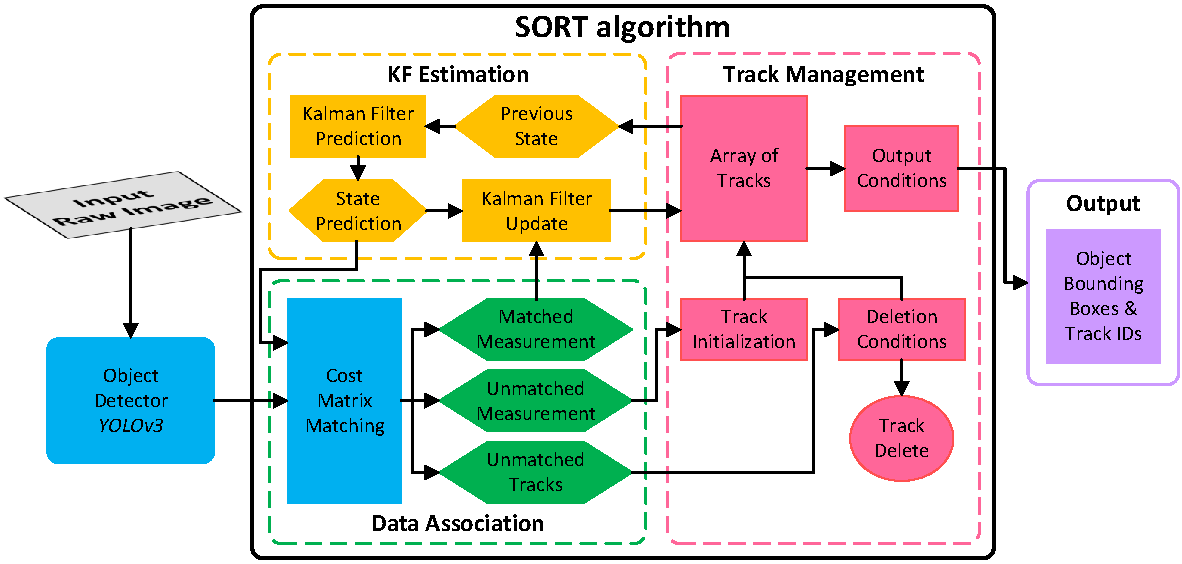
\includegraphics[width=1.0\textwidth]{obrazky-figures/SORT.pdf}
	\caption{Přehled architektury algoritmu SORT pro sledování objektů. Převzato z~článku~\cite{article:Tracking}.}
	\label{img:SORT}
\end{figure}

\subsection{DeepSORT}
\label{sec:DeepSORT}
DeepSORT\footnote{DeepSORT: \url{https://github.com/nwojke/deep_sort}}~\cite{website:Tracking} je vylepšení algoritmu SORT (viz~předchozí sekce~\ref{sec:SORT}) o~metrikou hloubkové asociace. Přestože SORT dosahuje celkově pozoruhodných výsledků v~přesnosti sledování, tak i přes účinnost Kalmanova filtru vrací poměrně mnoho kandidátních stop. To zapříčiňuje časté záměny identit, kterou dále znatelně ovlivňuje úhel pohledu~aj. Jako kompenzace tohoto nedostatku je v~tomto algoritmu zavedena další metrika, která je založená na \uv{vzhledu} objektu, a~tím tak vylepšuje proces asociace. Architektura tohoto algoritmu je zobrazena na obrázku~\ref{img:DeepSORT}.

Asociace detekovaných objektů~\cite{article:Tracking} ke stopám je i zde provedena pomocí Maďarského algoritmu stejně jako v~předchozím algoritmu SORT. DeepSORT ovšem nahrazuje asociační metriku za dvoudílnou porovnávací kaskádu. V~první části kaskády jsou použity metriky pohybu a~vzhledu pro přiřazení k~platným stopám, v~druhé části se pak používá stejná strategie jako v~algoritmu SORT pro asociaci nepřiřazených či nepotvrzených stop s~nepřiřazenými detekcemi.

Informace o~pohybu~\cite{article:Tracking} jsou začleněny v~kvadratické Mahalanobisové vzdálenosti mezi predikovanými oblastmi Kalmanova filtru a~současnými detekcemi. Tyto informace jsou užitečné zejména v~krátkodobé predikci. Pomocí této metriky~\cite{article:DeepSORT} je také možné vyloučit nepravděpodobné asociace prahováním vzdálenosti na $95$~\% míry jistoty. Metrika vzhledu je založená na nejmenší kosinusové vzdálenosti mezi stopami a~tzv.~\uv{deskriptory vzhledu}, které jsou zvláště užitečné pro obnovení stopy po dlouhodobých výpadcích, kdy je pohyb méně relevantní. Deskriptor vzhledu je spočítaný nad detekcí pomocí předtrénované KNN, která byla natrénovaná na rozsáhlém datasetu osob. Asociační metoda je potom definována kombinací těchto dvou metrik a~lze ji zapsat vztahem~\ref{eqn:DeepSORTmetric}.

\begin{equation}
    \label{eqn:DeepSORTmetric}
    D = \lambda \cdot D_{m} + (1 - \lambda) \cdot D_{c},
\end{equation}
kde $D_{m}$ je Mahalanobisová vzdálenost, $D_{c}$ je kosinusová vzdálenost a~$\lambda$ je váhový parametr.

\begin{figure}[hbt]
	\centering
	\setlength{\fboxsep}{0pt}
	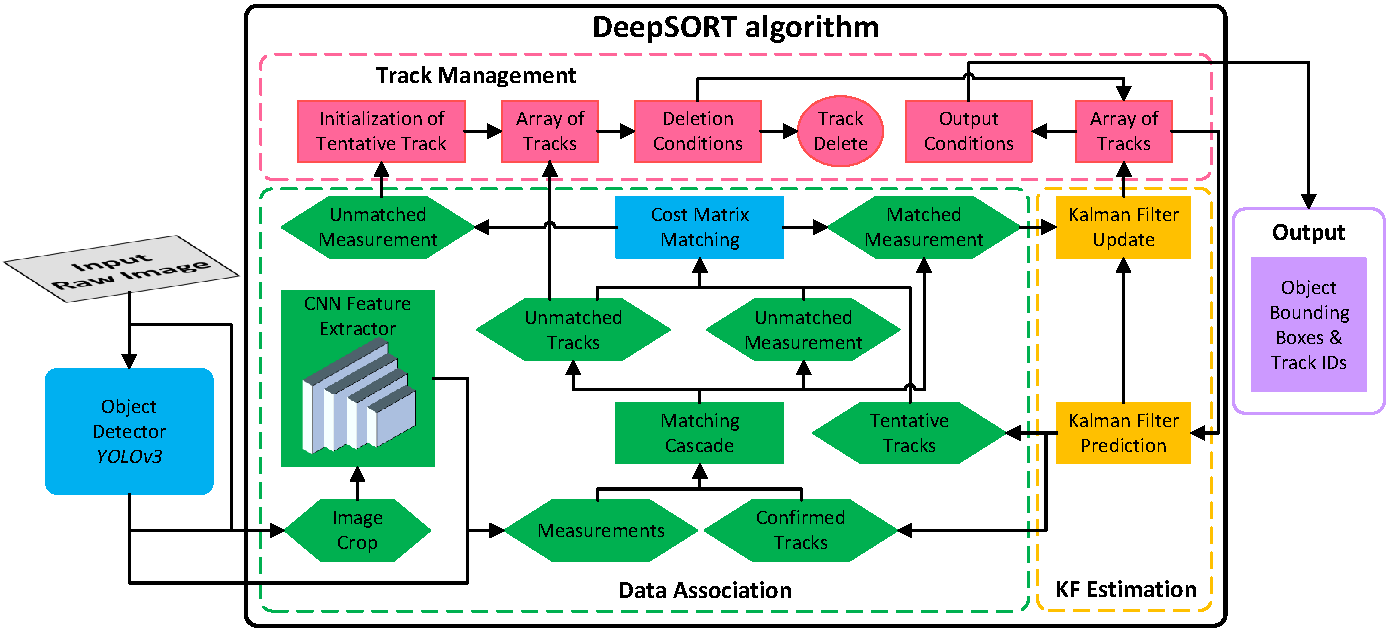
\includegraphics[width=1.0\textwidth]{obrazky-figures/DeepSORT.pdf}
	\caption{Přehled architektury algoritmu DeepSORT. Převzato z~článku~\cite{article:Tracking}.}
	\label{img:DeepSORT}
\end{figure}

\chapter{Technologie pro vývoj internetových aplikací}
\label{kap:technologie}
V následující kapitole budou detailněji popsány použité technologie při implementaci. Jako první je uvedeno prostředí Node.js, jelikož na něm staví další použité nástroje. Následující část je pak věnována frameworku Express.js a~jeho hlavním inovacím, které s~sebou do tohoto prostředí přináší, včetně způsobu, jakým zpracovává příchozí požadavky. Dále je text zaměřen na knihovnu React a~její principy pro vytváření uživatelského rozhraní. Tato sekce také podrobněji popisuje životní cyklus komponent a~jak se s~nimi zachází. Na konec jsou uvedeny komunikační technologie, které byly použity pro přenos dat jako jsou Socket.io a~REST API.

\section{Node.js}
\label{sec:Node}
Node.js\footnote{Node.js: \url{https://nodejs.org}}~\cite{book:NodeJS-WebDevelopment, book:LearningNode} je multi-platformní prostředí pro vývoj vysoce škálovatelných internetových aplikací, které je postaveno na JavaScriptovém open-source enginu V8\footnote{V8 engine: \url{https://v8.dev}}, jenž byl původně vytvořený pro Google Chrome. Tento engine byl vytvořen za účelem zvýšení rychlosti JavaScriptu začleněním \emph{\uv{just-in-time}} (JIT) kompilátoru, který kompiluje JavaScript do strojového kódu. Tím je umožněno používat JavaScript i~mimo prohlížeč a~vývojářům je tak dovoleno psát v~tomto jazyce nejen klientskou stranu aplikace, ale taktéž serverovou část. V~důsledku lze takto použít pouze jeden programovací jazyk na celou aplikaci a~prosadit tak paradigma \emph{\uv{JavaScript everywhere}}. Nejčastěji se ovšem Node.js používá pro vývoj síťových programů jako jsou webové servery, jelikož se drží neblokujícího, událostmi řízeného modelu.

\subsection{Architektura}
Běžné serverové systémy využívají \emph{\uv{one-thread-per-client}} přístup, kde s~každým novým požadavkem je vytvořeno nové vlákno, které daný požadavek obslouží (např.~Apache). Přestože tento přístup má své výhody, tak zatěžuje systémovou operační paměť a~je nutné také vzít v~úvahu režii spojenou s~vytvářením samotných vláken, obzvlášť v~případě, kdy požadavky obnášejí jednoduché, výpočetně nenáročné operace.

Na rozdíl tomu Node.js využívá velmi malé množství vláken k~obsluze všech příchozích požadavků. Tím jsou ušetřeny systémové prostředky spojené s~režií vláken a~lze tak strávit více času nad samotnými požadavky. Na druhou stranu, protože Node.js disponuje pouze několika vlákny, je nutné s~nimi zacházet moudře. Dělí se na dvě skupiny~--~Event loop (smyčku událostí) a~Thread pool.

Smyčka událostí~\cite{website:TheNodeArchitecture} je podstatnou částí Node.js, která umožňuje provádět asynchronní, neblokující operace. Obsahuje pouze jedno vlákno, které se stará o~všechny příchozí požadavky v~nekonečné smyčce (viz~obrázek~\ref{img:Libuv architektura}). Příchozí požadavky se řadí do fronty událostí a~hlavní vlákno ho buď vykoná, jedná-li se o~blokující operaci nebo ho předá ke zpracování volnému pracovnímu vláknu, které po dokončení asynchronní operace invokuje \emph{callback} funkci, která je opět zaslána zpět do vstupní fronty. Lze si povšimnout, že pro rychlý chod programu je nutné tuto smyčku událostí nezatěžovat náročnými blokujícími operacemi, protože by mohlo dojít k~jejímu zablokování a~tím k~zamrznutí programu.

Thread pool~\cite{website:TheNodeArchitecture} poskytuje dodatečná pracovní vlákna (v základu 4, ale lze konfigurovat až na 1024), na které může hlavní smyčka delegovat asynchronní či náročné požadavky včetně blokujících I/O operací. Typicky mezi takové požadavky patří přístup k~souborovému systému, databázím či síťové transakce~aj. O~celou tuto funkcionalitu včetně smyčky událostí se stará knihovna Libuv\footnote{Libuv: \url{https://libuv.org}}, která tvoří podstatnou část Node.js a~kde jsou tyto náročné operace většinou již asynchronně implementovány.

\begin{figure}[hbt]
	\centering
	\setlength{\fboxsep}{0pt}
	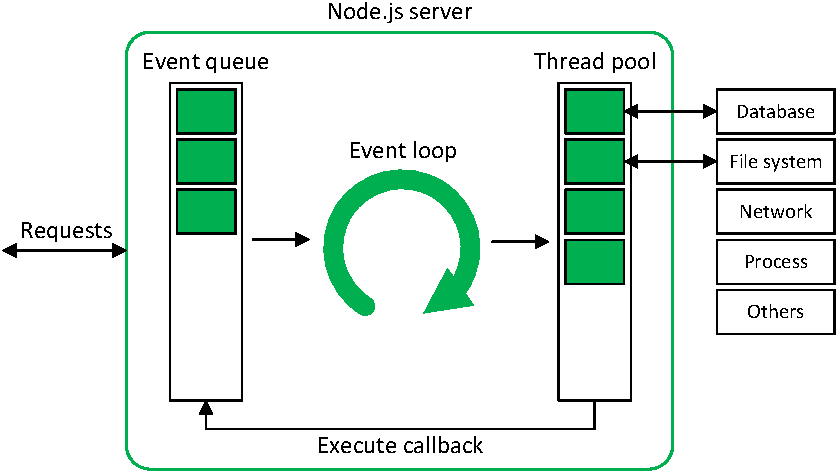
\includegraphics[width=1.0\textwidth]{obrazky-figures/LibuvArchitecture.pdf}
	\caption{Architektura knihovny Libuv pro obsluhu požadavků pomocí smyčky událostí. Převzato z~článku~\cite{website:TheNodeArchitecture}.}
	\label{img:Libuv architektura}
\end{figure}

Doposud byly zmíněny pouze závislosti Node.js na enginu V8 a~knihovně Libuv. Tyto dvě komponenty patří sice mezi nejdůležitější, ovšem nejsou jediné a~celou architekturu Node.js lze vidět na obrázku~\ref{img:Node.js architektura}. Mezi další závislosti~\cite{website:NodeJSArchitectureAndConcurrencyModel} patří:
\begin{itemize}
    \item \textbf{llhttp}\footnote{llhttp: \url{https://github.com/nodejs/llhttp}}~--~Knihovna pro parsování HTTP. Navržena tak, aby neprováděla žádná systémová volání či alokace.
    \item \textbf{c-ares}\footnote{c-ares: \url{https://c-ares.org}}~--~Knihovna pro asynchronní DNS požadavky použité v~DNS modulu.
    \item \textbf{OpenSSL}\footnote{OpenSSL: \url{https://www.openssl.org}}~--~Pro kryptografické funkce použité v~TLS (SSL) a~crypto modulech. Poskytuje mnoho funkcí, na které moderní weby spoléhají z~hlediska bezpečnosti.
    \item \textbf{zlib}\footnote{zlib: \url{https://zlib.net}}~--~Knihovna pro synchronní, asynchronní a~stream kompresi a~dekompresi.
\end{itemize}

\begin{figure}[hbt]
	\centering
	\setlength{\fboxsep}{0pt}
	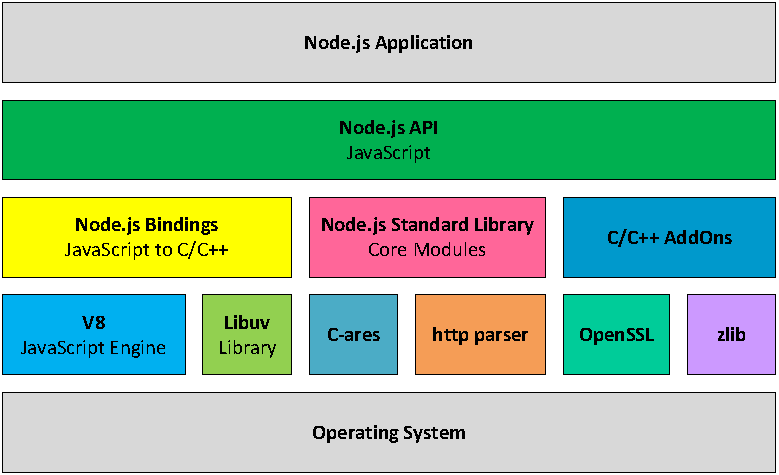
\includegraphics[width=0.9\textwidth]{obrazky-figures/NodeArchitecture.pdf}
	\caption{Architektura Node.js se všemi jejími závislostmi. Převzato z~článku~\cite{website:NodeJSArchitectureAndConcurrencyModel}.}
	\label{img:Node.js architektura}
\end{figure}

\subsection{Moduly}
Node.js~\cite{book:NodeJSDesignPatterns} umožňuje vývojářům definovat vlastní zapouzdřenou funkcionalitu a~šířit ji v~ekosystému modulů \emph{(packages)}, jenž se nachází mimo jádro Node.js. Tento princip má velký dopad na strukturu kódu programu a~kulturu tohoto prostředí, protože dává svobodu vývojářům experimentovat a~opakovat určitá existující řešení na problémy, se kterými se během vývoje potýkají. Spolu s~NPM (viz~následující sekce~\ref{sec:NPM}) pomáhá Node.js vyřešit konflikty v~závislostech tak, že každý nainstalovaný balíček má svoji vlastní oddělenou množinu závislostí. Tímto způsobem je možné zajistit velkou míru znovupoužitelnosti a~vytvářet nové aplikace podstatně rychleji. Moduly~\cite{website:NodeModules} se dělí do tří kategorií:
\begin{itemize}
    \item \textbf{Základní moduly}~--~Node.js má spoustu vestavěných modulu, které jsou již součástí prostředí a~jsou dodány během instalace.
    \item \textbf{Lokální moduly}~--~Na rozdíl od vestavěných a~externích modulů jsou lokální moduly vytvářeny přímo ve vyvíjené aplikaci a~zpřístupněny jiným souborům pomocí exportů.
    \item \textbf{Moduly třetích stran}~--~Jsou moduly, které jsou dostupné na internetu přes NPM. Tyto moduly mohou být nainstalovány přímo do projektu nebo také globálně.
\end{itemize}

\subsection{Node Package Manager}
\label{sec:NPM}
Velké množství funkcionality~\cite{book:LearningNode} spojené s~Node.js přichází prostřednictví modulů třetích stran. Tyto moduly lze nainstalovat manuálně do prostředí vyvíjené aplikace nebo pomocí specializovaného nástroje. Jedním z~těchto nástrojů je Node Package Manager\footnote{NPM: \url{https://www.npmjs.com}} (dále jen NPM), což je výchozí správce balíčků dodaný při instalaci Node.js, ačkoliv nemusí být vždy poskytnutý v~nejnovější verzi. NPM se ovšem neomezuje pouze na správu balíčku, ale taktéž nabízí kompletní správu projektu jako je definování vlastních příkazů, sledování závislostí balíčků či jejich zranitelností. Nově nainstalované balíčky přidává NPM do adresáře \texttt{node\_modules}.

NPM~\cite{thesis:WebApp} využívá ke správě projektu soubor \texttt{package.json}, ve kterém jsou obsažena metadata projetu. Zde je definován kromě jména projektu, verze, licence~aj. také seznam přímých závislostí projektu na jiných balíčcích, včetně jejich verze. Tento soubor je velmi důležitý a~musí být přenášen spolu s~aplikací, neboť při její sestavení v~novém prostředí se znovu podle něj stáhnou zde definované balíčky v~odpovídajících verzích a~sestaví se nový strom závislostí.

Dalším podstatným souborem je \texttt{package-lock.json}~\cite{thesis:WebApp}, který obsahuje přesný strom závislostí, jenž zaručuje kompletně shodné závislosti všech balíčků v~totožných verzích při opětovném sestavení aplikace. Rozdíl oproti klasickému sestavení je v~tom, že nebudou zaručeny pouze stejné verze přímých závislostí, ale taktéž závislosti těchto závislostí. To umožňuje pokaždé sestavit identický celý strom. Tento soubor je automaticky generovaný NPM při modifikaci souboru \texttt{package.json} nebo adresáře \texttt{node\_modules}, ovšem již není nutný k~sestavení a~používá se spíše při vývoji průběžných integrací do aplikace od více vývojářů.

\section{Express.js}
\label{sec:Express}
Express.js\footnote{Express.js: \url{https://expressjs.com}} (dále jen Express)~\cite{book:WebDevNodeAndExpress, book:ProExpress} je minimalistický a~flexibilní webový framework postavený na základu Node.js. Je určený především k~vývoji internetových aplikací či API, ale postupem času se stal de facto standardním serverovým aplikačním rámcem pro Node.js. Totiž běžný proces vývoje serveru postaveného pouze na Node.js zahrnuje stále opakující se a~zdlouhavé úkony jako je analýza těl HTTP požadavků, správa sezení, cookies, extrahování parametrů z~URL~aj. Express se snaží tyto rutinní činnosti více abstrahovat a~poskytnout tak způsoby k~jejich elegantnímu řešení.

Přestože Express~\cite{book:WebDevNodeAndExpress} v~základu poskytuje jen minimální rámec klíčových funkcí, je také velmi snadno rozšiřitelný. Jelikož se stále jedná o~framework postavený na Node.js a~o~JavaScript, je možné snadno zpřístupnit balíčky třetích stran pomocí NPM a~přidat tak pouze to, co je nutné. Některé balíčky jsou navíc vytvořeny výhradně pro funkce Expressu, ale obecně lze využít každý balíček pro Node.js.

\subsection{Middleware}
Middleware~\cite{book:WebDevNodeAndExpress, book:ExpressInAction} jsou funkce, které se provádějí během životního cyklu požadavku na serveru v~tzv.~\emph{\uv{pipeline}}, kde záleží na pořadí. Toto zřetězení umožňuje rozdělit logiku kódu na menší celky a~vytvořit tak znovupoužitelné middleware funkce. Ve skutečnosti samotný Express je takto sestavený výhradně z~middlewaru (viz~obrázek~\ref{img:ExpressMiddleware}). Funkce mají parametry \texttt{request} a~\texttt{response} objekty pro každou cestu, ke které je připojená a~parametr \texttt{next}, což je funkce. Každá middleware funkce může provádět následující:

\begin{itemize}
    \item Spustit libovolný kód pro obsluhu požadavku.
    \item Provést změny v~objektech požadavku a~odpovědi.
    \item Ukončit životní cyklus požadavku.
    \item Zavolat další middleware v~zásobníku pomocí funkce \texttt{next}.
\end{itemize}

\begin{figure}[hbt]
	\centering
	\setlength{\fboxsep}{0pt}
	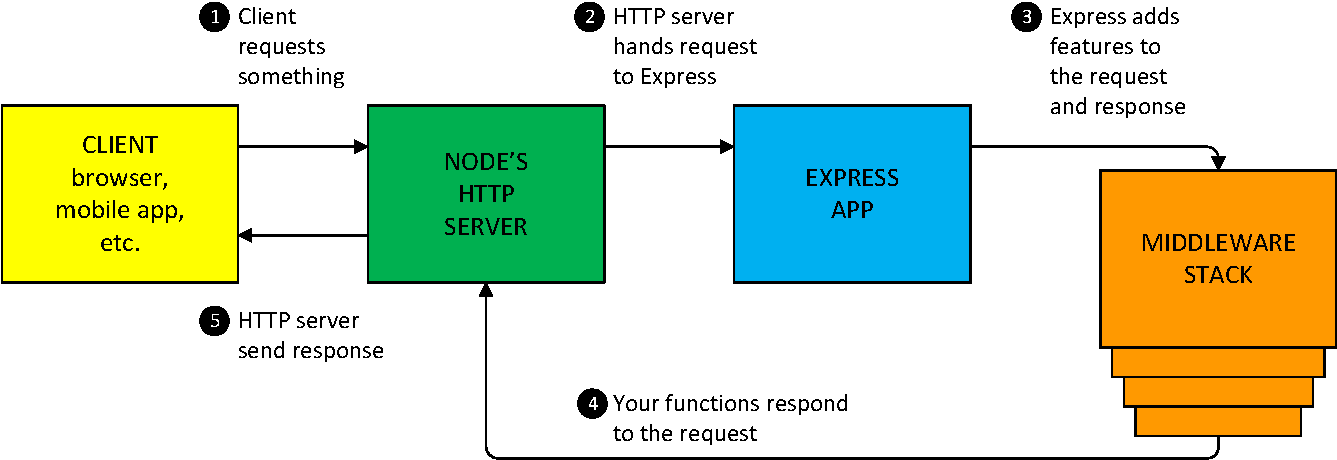
\includegraphics[width=1.0\textwidth]{obrazky-figures/ExpressRequestLifecycle.pdf}
	\caption{Diagram znázorňující životní cyklus požadavku, který je na straně Expressu zpracován pomocí sekvence middlewaru. Převzato z~knihy~\cite{book:ExpressInAction}.}
	\label{img:ExpressMiddleware}
\end{figure}

\subsection{Směrování}
Směrování \emph{(routing)}~\cite{book:ExpressInAction, book:ProExpress} umožňuje definovat koncové body \emph{(endpoints)}, kam mohou uživatelé zasílat své požadavky pomocí URI a~specifické HTTP metody. Každý koncový bod má poté jednu či více obslužných funkcí (jako middleware), které jsou postupně za sebou provedeny, pokud dojde k~jejich kompletní shodě. Express mimo jiné dovoluje organizovat tyto cesty do menších sekcí zvaných \emph{\uv{routers}}. Definice koncového bodu má potom formát tak, jak je uvedeno v~následujícím výpisu~\ref{vyp:ExpressEndpoint}.
\begin{center}
    \begin{lstlisting}[escapechar=@, label={vyp:ExpressEndpoint}, caption={Struktura definice koncového bodu v~Express.js. Kde \texttt{app} je instance třídy express, \texttt{method} je použitá HTTP metoda požadavku, \texttt{path} je cesta na serveru ke koncovému bodu a~\texttt{handler} je obslužná funkce.}]
        app.@\textcolor{codepurple}{method}@(@\textcolor{codeyellow}{path}@, @\textcolor{purple}{handler}@)
    \end{lstlisting}
\end{center}

\section{React}
\label{sec:React}
React\footnote{React: \url{https://reactjs.org}} je open-source JavaScriptová knihovna pro tvorbu uživatelského rozhraní, která je velmi dobře optimalizována pro práci s~často měnícími se daty. Zejména se používá při tvorbě jednostránkových aplikací tzv.~SPAs \emph{(Single Page Applications)}, mobilních aplikací pomocí React Native\footnote{React Native: \url{https://reactnative.dev}} nebo desktopových aplikací využívajících Electron\footnote{Electron: \url{https://www.electronjs.org}}. 

Aplikace implementované v~Reactu~\cite{book:LearningReact, website:EverythingReact} umožňují zápis v~JavaScriptovém rozšíření JSX (viz~výpis~\ref{vyp:reactElementJSX}), jenž se používá k~definici toho, jak má uživatelské rozhraní vypadat. Syntax je velmi podobný HTML či XML, ale doopravdy se jedná pouze o~syntaktický cukr, jehož cílem je zajistit čitelnější definice React elementů. Webové prohlížeče ovšem této syntaxi nerozumí a~je tedy nutné ji před nasazením na web přeložit. 

O tuto část se stará Babel\footnote{Babel: \url{https://babeljs.io}}~\cite{book:LearningReact}, což je JavaScriptový transpilátor, který se hlavně používá pro převod ECMAScriptu 2015+ (ES6+) do zpětně kompatibilních verzí JavaScriptu, které mohou být spuštěné na starších enginech (např.~v~prohlížečích). Kromě toho Babel umožňuje také převádět JSX do prostého JavaScriptu (viz~výpis~\ref{vyp:reactElementJS}). Samotný React však JSX syntax nevyžaduje a~je možné psát přímo v~čistém JavaScriptu, ale v~praxi se tento přístup příliš nevyužívá~--~viz~následující příklad:

\begin{center}
    \begin{lstlisting}[escapechar=@, label={vyp:reactElementJSX}, caption={Definice elementu v~syntaxi JSX.}]
        <@\textcolor{codeyellow}{MyButton}@ color="blue" shadowSize={@\textcolor{blue}{2}@}>
            Click Me
        </@\textcolor{codeyellow}{MyButton}@>
    \end{lstlisting}
\end{center}

\begin{center}
    \begin{lstlisting}[escapechar=@, label={vyp:reactElementJS}, caption={Ekvivalentní zápis elementu z~výpisu~\ref{vyp:reactElementJSX} v~JavaScriptu.}]
        @\textcolor{blue}{React}@.@\textcolor{codeyellow}{createElement}@(
            MyButton,
            {color: 'blue', shadowSize: @\textcolor{blue}{2}@},
            'Click Me'
        )
    \end{lstlisting}
\end{center}

\subsection{Objektový model dokumentu}
Objektový model dokumentu (dále jen DOM z~ang. názvu \emph{\uv{Document Object Model}})~\cite{thesis:WebApp} je standardní a~objektově orientovaná reprezentace HTML/XML dokumentu ve stromové struktuře, kde každý element v~dokumentu je v~této hierarchii reprezentován odpovídajícím uzlem. Tím, že tento formát je takto logicky strukturovaný, je umožněno snadno měnit obsah či pracovat s~konkrétní částí dokumentu přímo z~JavaScriptu.

Manipulace s~DOM~\cite{website:ReactVirtualDOM} je ovšem nákladná operace, jelikož pokaždé, když se změní stav programu, musí se strom znovu upravit a~překreslit uživatelské rozhraní, aby byly uživateli reflektovány nové změny. Nejde ani tak o~samotnou aktualizaci stromové struktury, jelikož na to již existuje spousta rychlých algoritmů. Co se ukazuje jako nákladné je fakt, že se musí znovu překreslit aktualizovaný element a~celý jeho podstrom, zejména pokud daný podstrom obsahuje velké množství dalších elementů.

React se snaží tomuto problému předcházet a~využívá koncept zvaný \textbf{virtuální DOM}. Virtuální DOM~\cite{website:ReactVirtualDOM} je vlastně odlehčená kopie reálné DOM reprezentace a~tedy každý uzel v~reálném stromě má zastoupení i~v~tom virtuálním, s~tím rozdílem, že provedené změny ve virtuální reprezentaci nejsou vykresleny na obrazovku uživatele. Díky této vlastnosti je práce s~virtuálním DOM časově velmi efektivní. Ve skutečnosti to probíhá tak, že před každou novou změnou stavu v~programu, React vytvoří kopii aktuálního virtuálního DOM pomocí \emph{\uv{snapshotu}} a~poté tuto kopii modifikuje. Následně porovná aktuální a~upravenou verzi a~detekuje rozdíly. Nakonec jsou tyto rozdíly aktualizovány v~reálném DOM tím nejlepším možným způsobem. Tento proces se také nazývá \emph{\uv{diffing}} a~může připomínat aplikaci opravného patche.

React s~optimalizací však zachází ještě dále a~provádí aktualizace stavu po dávkách \emph{(batch update)} za účelem zvýšení výkonu aplikace. Stav programu se totiž provádí asynchronně a~React tak při každé aktualizaci stavu ještě chvíli vyčkává na případné další nové změny a~poté tyto změny překreslí zároveň.

\subsection{Komponenty}
Komponenty jsou základní, nezávislé a~opakovaně použitelné části kódu, které slouží k~definici uživatelského rozhraní a~umožňují ho dekomponovat na menší části. Výsledná kompozice komponent má potom stromovou strukturu, kde kořen stromu je komponenta na nejvyšší úrovni, která je potom při překladu napojena na výchozí prvek (\texttt{div} element s~identifikátorem \texttt{root}) ve vstupním bodě aplikace. Každá komponenta může mít vstupy (nazývané \emph{\uv{properties}} zkr. \emph{\uv{props}}) či vlastní stav a~musí vracet React elementy. 

Vstupy slouží k~distribuci dat napříč aplikací a~jsou určeny pouze ke čtení. React používá tzv.~jednosměrnou datovou vazbu a~vzhledem k~tomu, že komponenty jsou organizovány do stromové struktury, tak může pouze nadřazená komponenta zpřístupnit hodnoty své přímo podřízené komponentě. Opačný směr předávání dat je možný jen přes referenci, ale většinou tento přístup nepatří mezi dobré zásady. 

Stav~\cite{thesis:WebApp} naopak umožňuje komponentě spravovat vlastní data, která nelze číst a~nastavit mimo danou komponentu. Data uložená ve stavu jsou typicky zobrazována uživateli a~postupem času se mění při interakci s~aplikací pomocí událostí. Kdykoliv dojde k~aktualizaci stavu či vstupu, bude komponenta znovu překreslena. Z~hlediska stavu se pak komponenty dělí na:

\begin{itemize}
    \item \textbf{Bezstavové}
        \begin{itemize}
            \item Nemají žádný stav
            \item Můžou mít vstupy
            \item Překreslení je závislé pouze na vstupech
        \end{itemize}
    \item \textbf{Stavové}
        \begin{itemize}
            \item Mají vlastní stav
            \item Můžou mít vstupy
            \item Překreslení je závislé na vstupech a~stavu
        \end{itemize}
\end{itemize}

Samotné komponenty~\cite{website:ReactComponents} lze implementovat ve funkcionálním nebo třídním zápisu. Na první pohled je nejvýznamnějším rozdílem syntax, kde funkcionální komponenty jsou jednodušší na porozumění, jelikož se jedná o~obyčejné JavaScriptové funkce, které vrací React elementy (viz~výpis~\ref{vyp:funkcionalniKomponenta}). Třídní komponenty jsou zase JavaScriptové třídy, které rozšiřují třídu \texttt{React.Component} o~implementaci metody \texttt{render()}, která opět musí vracet elementy Reactu (viz~výpis~\ref{vyp:tridniKomponenta}).

\begin{center}
    \begin{lstlisting}[escapechar=@, label={vyp:funkcionalniKomponenta}, caption={Funkcionální komponenta definovaná pomocí šipkové notace.}]
        const @\textcolor{codepurple}{MyComponent}@ = (props) => {
            return <@\textcolor{codeyellow}{h1}@>Hello, {props.name}</@\textcolor{codeyellow}{h1}@>;
        };
    \end{lstlisting}
\end{center}

\begin{center}
    \begin{lstlisting}[escapechar=@, label={vyp:tridniKomponenta}, caption={Ekvivalentní definice výpisu~\ref{vyp:funkcionalniKomponenta} v~třídní komponentě.}]
        class @\textcolor{purple}{MyComponent}@ extends @\textcolor{purple}{React.Component}@ {
            @\textcolor{codeyellow}{render}@() {
                @\textcolor{codepurple}{return}@ <@\textcolor{codeyellow}{h1}@>Hello, {this.props.name}</@\textcolor{codeyellow}{h1}@>;
            }
        }
    \end{lstlisting}
\end{center}

Dříve se funkcionální zápis používal pouze k~definici bezstavových komponent a~tyto komponenty poskytovaly vyšší výkon. Ovšem od verze $16.8$ disponují funkcionální komponenty i~React Hooky, což jim umožňuje využívat mechaniky jako jsou vstupy, stavy, reference, přístup k~událostem z~životního cyklu komponenty~aj. Nyní jsou funkcionální komponenty stejně silné jako třídní komponenty (i z~hlediska výkonu).

\subsection{Životní cyklus komponent}
Každá komponenta má vlastní životní cyklus, který lze definovat jako sérii událostí, které jsou vyvolávány v~různých fázích její existence. Díky tomu je možné v~tomto procesu pomocí metod definovat její chování. Tyto metody jsou také známé jako metody životního cyklu a~využívají se v~třídních komponentách (viz~obrázek~\ref{img:ReactComponentLifecycle}). Funkcionální zápis umožňuje přístup k~těmto událostem pomocí React Hooků a~nabízejí tak podobnou funkcionalitu. Každá komponenta~\cite{website:ReactComponentsLifecycle, website:ComponentsLifecycleInReact, thesis:WebApp} prochází následujícími třemi fázemi:

\begin{enumerate}
    \item \textbf{Montáž} \emph{(Mounting)}~--~je první fáze v~životním cyklu, kde komponenta je přidána do DOM a~poprvé vykreslena. Zde je zavolán její konstruktor, inicializován její stav a~vstupy. Během této fáze jsou dostupné tyto metody:
    \begin{enumerate}
        \item \texttt{constructor()}~--~první zavolaná metoda předtím, než je komponenta namontována. Typicky se využívá pro inicializaci stavu a~navázání metod pro obsluhu událostí na instanci.
        \item \texttt{static getDerivedStateFromProps()}~--~tato metoda je zavolána vždy těsně předtím, než je komponenta vykreslena. Využívá se u~vzácných případů, kdy stav komponenty závisí na změnách na vstupech.
        \item \texttt{render()}~--~tato metoda vrací obsah, jenž bude vykreslen do prohlížeče (React elementy). Uvnitř této metody by nemělo docházet ke změně stavu komponenty ani k~přímé interakci s~prohlížečem.
        \item \texttt{componentDidMount()}~--~metoda je zavolána ihned potom, co je komponenta namontována do DOM. Zde je možné dodatečně změnit stav komponenty, ještě předtím než bude aktualizováno uživatelské rozhraní, což sice způsobí dodatečné překreslení, ale uživatel neuvidí mezistav.
    \end{enumerate}
    
    \item \textbf{Aktualizace} \emph{(Updating)}~--~v~této fázi se komponenta vyskytuje při překreslení způsobeného změnou stavu nebo vstupu.
    \begin{enumerate}
        \item \texttt{static getDerivedStateFromProps()}~--~metoda je zavolána vždy před překreslením komponenty (viz~výše). 
        \item \texttt{shouldComponentUpdate()}~--~je pravdivostní metoda, která těsně před překreslením komponenty rozhoduje o~tom, zda k~němu dojde či nikoliv. Používá se k~optimalizačním účelům a~ve výchozím nastavení je návratová hodnota nastavena vždy na \texttt{true}.
        \item \texttt{render()}~--~opět vykreslující metoda, jenž definuje podobu komponenty (viz~výše).
        \item \texttt{getSnapshotBeforeUpdate()}~--~tato metoda je zavolána předtím, než budou provedeny změny v~reálném DOM. Umožňuje komponentě zachytit některé informace z~virtuálního DOM o~výsledném rozložení a~slouží tak jako poslední kontrola předtím, než se samotná data opravdu vykreslí.
        \item \texttt{componentDidUpdate()}~--~metoda je zavolána ihned po aktualizaci všech změn v~reálném DOM.
    \end{enumerate}
    
    \item \textbf{Odpojení} \emph{(Unmounting)}~--~během této fáze dochází k~odstranění komponenty ze struktury DOM.
    \begin{enumerate}
        \item \texttt{componentWillUnmount()}~--~metoda je invokována těsně před odpojením a~následným zničením komponenty. Umožňuje tak dodatečně uvolnit alokované zdroje.
    \end{enumerate}
\end{enumerate}

\begin{figure}[hbt]
	\centering
	\setlength{\fboxsep}{0pt}
	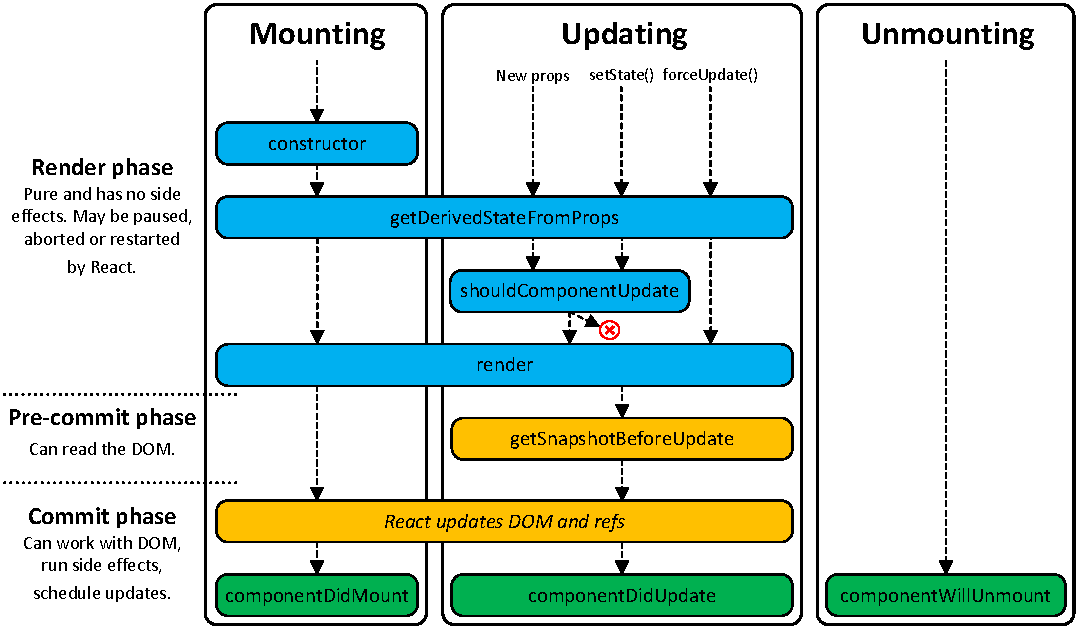
\includegraphics[width=1.0\textwidth]{obrazky-figures/ReactComponentLifecycle.pdf}
	\caption{Životní cyklus komponent ve třech fázích. V~každé fázi je zobrazena sekvence výskytu metod životního cyklu tak, jak na sebe chronologicky navazují. Převzato z~článku~\cite{website:ReactComponentsLifecycle}.}
	\label{img:ReactComponentLifecycle}
\end{figure}

\section{Socket.io}
\label{sec:SocketIO}
Socket.io\footnote{Socket.io: \url{https://socket.io}}~\cite{manual:SocketIO} je JavaScriptová knihovna implementující vrstvu řízenou událostmi pro obousměrnou, stavovou komunikaci mezi klientem a~serverem. Je postavena na knihovně nižší úrovně Engine.io\footnote{Engine.io: \url{https://github.com/socketio/engine.io}} a~abstrahuje přenos dat pomocí HTTP long-polling a~WebSocketů do jediného API, jenž má širokou podporu napříč prohlížeči. Kromě běžné komunikace knihovna také poskytuje další užitečné vlastnosti jako je automatická obnova spojení při výpadku a~ukládání paketů do vyrovnávací paměti, broadcastování všem klientům nebo jejich podmnožině, rozdělení logiky pomocí jmenných prostorů, podpora streamování binárních dat~aj.

K vytvoření spojení~\cite{manual:SocketIO} knihovna nejdříve používá dotazování pomocí xhr-pollingu, jakmile je toto spojení navázáno, tak použije nejlepší dostupnou metodu komunikace~--~ve většině případů právě WebSocket. Ve výchozím nastavení Socket.io před samotným vylepšením metody však ještě nějaký čas používá transport přes HTTP polling. Ukázalo se totiž, že komunikaci přes WebSockety není možné vždy úspěšně navázat navzdory své široké podpoře kvůli firemním proxy serverům, firewallům, antivirovým programům~aj. Toto neúspěšné navázání se pak může promítnout až do $10$-ti sekundového čekání, než započne výměna dat. Pro vylepšení metody klient musí provést následující:
\begin{enumerate}
    \item Ujistit se, že jeho odchozí buffer je prázdný.
    \item Nastavit aktuální přenos do režimu pouze pro čtení.
    \item Pokusit se navázat přenos pomocí nové metody.
    \item V~případě úspěchu uzavřít původní spojení.
\end{enumerate}

\section{REST API}
Representational State Transfer (REST)~\cite{website:REST} je architektonický styl pro komunikaci mezi klientem a~serverem. Obsahuje soubor pravidel, které definuje rozhraní API a~způsob jakým klient přistupuje k~datům. Data se označují jako zdroje a~přístup k~nim je umožněn přes endpointy, ke kterým uživatel přistupuje pomocí konkrétní URL. Poté co uživatel odešle na tento koncový bod svůj požadavek, je na serveru provedena příslušná operace a~vrácena konkrétní odpověď. REST ke komunikaci nejčastěji používá následujících pět HTTP metod:
\begin{itemize}
    \item \textbf{GET}~--~Poskytne přístup ke čtení zdroje.
    \item \textbf{POST}~--~Vytvoří nový zdroj.
    \item \textbf{PUT}~--~Aktualizuje existující zdroj jeho nahrazením.
    \item \textbf{PATCH}~--~Aktualizuje existující zdroj jeho částečnou modifikací.
    \item \textbf{DELETE}~--~Odstraní zdroj.
\end{itemize}

Požadavek~\cite{website:REST} kromě adresy koncového bodu a~metody, také obsahuje hlavičky a~tělo. Hlavičky se používají k~poskytnutí dodatečných informací s~HTTP požadavkem jak klientovi, tak serveru například o~formátu nesených dat. Existuje více druhů hlaviček a~jsou vždy v~páru klíč-hodnota. Tělo neboli data pak obsahují informace, které daný požadavek s~sebou nese. Tato část se však nepoužívá u~metody \texttt{GET}. Samotný REST je bezstavový, což znamená, že na straně serveru není uložen žádný kontext či historie předchozí komunikace s~klientem. Každý požadavek od klienta proto musí obsahovat všechny náležité informace, aby server byl schopný na něj správně reagovat.


\chapter{Návrh a~implementace}
\label{kap:implementace}
Tato kapitola je zaměřena na návrh a~implementaci aplikace pro detekci narušitelů. Na začátku je popsána obecná architektura řešení, z~jakých částí se skládá a~jak se mezi nimi data zasílají. V~další části je uvedena výsledná podoba klientské části, která je doplněna o~některé implementační detaily. Následující sekce je pak věnována implementaci serveru, která popisuje komunikaci s~klientem, způsob, jakým se data ukládají a~jak se s~nimi následně pracuje. Na závěr této kapitoly je podrobněji sepsán proces pro zpracování videozáznamu, včetně detailů všech hlavních komponent, kterými disponuje.

\section{Návrh architektury}
Jak již bylo zmíněno v~úvodní kapitole, tak aplikace je navržena typu klient-server ve webovém rozhraní. Uživatel prostřednictvím prohlížeče načte veškerá potřebná data a~nakonfiguruje způsob zpracování videozáznamu. Data jsou následně odeslána na server, kde se celý záznam zpracuje. Zpracovaný záznam spolu s~výpisem detekovaných objektů bude na konci pak vrácen zpět ke klientovi, který si ho bude moci přehrát či stáhnout. Celý návrh architektury je možné vidět na obrázku~\ref{img:navrh}.

\begin{figure}[hbt]
	\centering
	\setlength{\fboxsep}{0pt}
	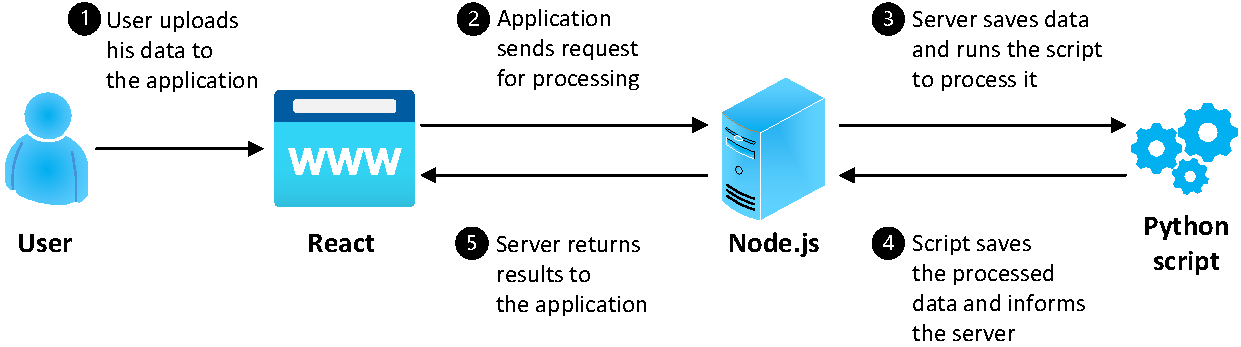
\includegraphics[width=1.0\textwidth]{obrazky-figures/navrh.pdf}
	\caption{Návrh architektury internetové aplikace.}
	\label{img:navrh}
\end{figure}

Klientská strana je implementována pomocí JavaScriptové knihovny React (viz~sekce~\ref{sec:React}), jelikož je dobře optimalizována pro práci s~často měnícími se daty, umožňuje snadnou dekompozici a~také usnadňuje její implementaci. Uživatel v~aplikaci po načtení svého záznamu pak nastaví podrobnosti ohledně jeho dalšího zpracování jako např.~vymezí na záznamu sledovanou oblast, nahraje vlastní detektor nebo snímky obličejů pro identifikaci osob~aj. Na konci této fáze budou data s~konfigurací odeslána na server, kde proběhne zpracování.

Na straně serveru, postaveného na Node.js (viz~sekce~\ref{sec:Node}), jsou přijatá data dočasně uložena tak, aby k~nim byl umožněn přístup skriptu, který celé video zpracuje. Důležité v~tomto procesu je rozlišovat data od klientů a~ukládat je odděleně tak, aby nedocházelo ke konfliktům a~žádná data nijak nezasahovala mezi data jiného klienta. To by při současném zpracování více záznamů mohlo v~důsledku zapříčinit, že by na konkrétním záznamu mohly být rozpoznávány osoby i~podle snímků obličeje, které nahrál jiný uživatel.

Skript pro zpracování videa je implementován v~pythonu a~zpracování probíhá po jednotlivých snímcích. Na každém snímku jsou jako první detekovány a~následně klasifikovány objekty, jež mohou být považovány za narušitele pomocí detektoru YOLO (viz~sekce~\ref{sec:YOLO}). Pokud narušitelem bude osoba, tak dojde k~její identifikaci pomocí systému DeepFace (viz~sekce~\ref{sec:DeepFace}) vůči databázi se snímky obličejů nahraných od uživatele. Každý snímek obličeje obsahuje jméno osoby, které v~případě shody bude zobrazeno na videu. Ostatní detekované objekty jsou pak označeny pouze jejich třídou, confidence skóre, případně unikátním identifikátorem při nastaveném sledování objektů.

Během procesu zpracování jsou uživateli pravidelně zasílány informace o~aktuálním postupu pro predikci zbývajícího času. Nakonec jsou data zaslána zpět do klientské části, kde je k~dispozici zpracované video spolu se souhrnem výsledků s~detekovanými objekty a~zaznamenanými časy.

\section{Návrh a~implementace aplikace}
Aplikace je rozdělena na řadu jednotlivých kroků, kterými musí uživatel postupně projít, než bude moci svůj záznam úspěšně odeslat ke zpracování. Tento způsob zejména usnadňuje orientaci v~aplikaci tím, že každý krok přímo popisuje, jaká akce se od uživatele očekává a~celý proces nepůsobí tak chaoticky. Zároveň je tímto způsobem ošetřené pořadí některých úkonů, které nelze zaměnit, např.~výběr sledované oblasti není možný bez toho, aniž by byl předtím nahraný záznam. Celý proces konfigurace je zároveň u~jednotlivých operací doplněný poznámkami a~dodatečnými popisky.

V prvním kroku musí uživatel nahrát svůj záznam (viz~obrázek~\ref{img:appImages1}), tato část je povinná a~není možné bez ní pokračovat. Poté co uživatel vloží video, zobrazí se v~přehrávači včetně jeho metadat a~povolí se postup do dalšího kroku. V~druhém kroku uživatel navolí konfiguraci, jak má být jeho záznam zpracován. Podstatou celého zpracování je detekce potencionálních narušitelů, proto detekci objektů nelze vypnout a~slouží tak spíše jako symbol indikující, že detekce proběhne vždy, i~když uživatel zakáže ostatní možnosti. Lze však dodatečně deaktivovat detekci vozidel pro případ, kdy by byl záznam pořízen z~oblasti, ve které se vozidla běžně vyskytují a~nelze je tak považovat za \uv{podezřelé} jevy (např.~kamerový záznam z~domovní příjezdové cesty, kde obyvatelé obvykle parkují nebo záznam z~firemního areálu, které zároveň slouží jako parkoviště). Dále u~samotné detekce je možné nastavit její přesnost. Tato možnost definuje, v~jakém rozlišení budou snímky vkládány do neuronové sítě, která provádí detekci. Vyšší rozlišení tak zajistí přesnější ohraničení objektů, ovšem znatelně prodlouží dobu na zpracování celého záznamu.

\begin{figure}[hbt]
	\centering
	\setlength{\fboxsep}{0pt}
	\includegraphics[width=1.0\textwidth]{obrazky-figures/appImages1.png}
	\caption{Ukázka aplikace, kde vlevo a~uprostřed je zobrazen první krok pro nahrání videa a~napravo se nachází nastavení konfigurace pro zpracování.}
	\label{img:appImages1}
\end{figure}

Další dostupnou volbou, která má vliv na dobu zpracování je rozpoznávání osob podle obličejů. V~tuto chvíli dojde pouze k~aktivaci tohoto modulu, ale na nahrání snímků dojde až v~pozdější části celého procesu. Poslední volbou ovlivňující výkon je sledování objektů (alias \emph{tracking}). Tento modul ke každé detekci přiřadí unikátní identifikátor a~umožní k~nim ukládat dodatečné informace napříč snímky. Tím se pak povoluje možnost i~jednotlivé objekty na snímku počítat nebo vykreslovat za nimi cesty a~zobrazit tak trasu odkud přišly. U~cest je zde také možnost specifikovat její délku v~sekundách, po které začne opět mizet. Sledování objektů v~kombinaci s~rozpoznáváním obličejů umožní po identifikaci osoby udržet její jméno zobrazené i~po tom, co osoba zahalí svůj obličej. Poslední parametr pak umožňuje na každý snímek vypsat aktuální čas na záznamu.

V následujícím kroku může uživatel na záznamu vymezit sledovanou oblast a~tím zamezit detekci objektů, které se nachází mimo ni (viz~obrázek~\ref{img:appImages2}). Zobrazený snímek pro vymezení oblasti je vygenerován náhodně při vložení záznamu a~lze ho případně kdykoliv změnit, pokud by z~nějakého důvodu nevyhovoval. Oblast je pak reprezentována souřadnicemi levého horního rohu, svojí šířkou a~výškou (minimálně však $50\times50$ pixelů). Tato oblast je definovaná pro všechny snímky a~je možné i~nastavit, aby byla či nebyla znázorněna na zpracovaném záznamu.

V předposledním kroku je uživateli umožněno nahrát snímky obličejů, které budou vloženy do databáze a~použity pro rozpoznávání detekovaných osob. Počet snímku není nijak omezený, ale je doporučeno nahrát ke každé osobě aspoň pět snímků tváří včetně čelního pohledu, kde každý snímek je pootočený o~$45$ stupňů. U~každé osoby je kromě snímků nutné zadat její jméno a~příjmení, které bude v~případě identifikace vykresleno uvnitř odpovídajícího bounding boxu. Duplicity jmen jsou povoleny, protože interně je každá osoba reprezentována unikátním identifikátorem.

\begin{figure}[hbt]
	\centering
	\setlength{\fboxsep}{0pt}
	\includegraphics[width=1.0\textwidth]{obrazky-figures/appImages2.png}
	\caption{Vlevo se nachází krok v~aplikaci pro zvolení detekční oblasti, uprostřed je krok pro nahrání snímků obličeje do databáze a~vpravo je zobrazen poslední krok s~nahranými váhami neuronové sítě.}
	\label{img:appImages2}
\end{figure}

Poslední krok umožňuje nahrát vlastní váhy pro neuronovou síť YOLOv3, které se použijí na zpracování daného záznamu. Důležité je, aby váhy byly dotrénovány na již předtrénovaných vahách na datasetu COCO\footnote{COCO: \url{https://cocodataset.org}} a~umožnily tak detekci všech základních $80$-ti~tříd. Pokud budou nahrány nekompatibilní váhy, aplikace informuje uživatele o~chybě. Tato možnost je tu pro případ, kdyby uživatel disponoval lepším detektorem pro danou scénu na záznamu, mohl by tak zlepšit přesnost detekcí. Původně bylo v~aplikaci plánováno nahrát pouze trénovací, anotovaná data a~dotrénovat detektor na straně serveru. Ovšem tento přístup by znatelně zatěžoval server na dlouhou dobu a~tím by se pak omezil výkon i~ostatním uživatelům. Uživatel po tomto kroku může odeslat data na server a~zahájit zpracování.

Během zpracování je uživatel informován o~aktuálním postupu pomocí ukazatelů průběhu (viz~obrázek~\ref{img:appImages3}). Poté co je video úspěšně zpracováno, je uživatel automaticky přesměrován na další obrazovku s~výsledky. Výsledná obrazovka obsahuje zpracované video, které je možné ihned přehrát ve webovém přehrávači nebo ho stáhnout. Níže se nachází seznam nalezených objektů, kde každá záložka představuje konkrétní třídu objektu a~po jejím rozbalení jsou zobrazeny časy, ve kterých byl objekt na záznamu spatřen. Po kliknutí na daný čas pak bude video automaticky přetočeno na tuto detekci. Osoby, pro které byly nahrány snímky obličejů a~byly na záznamu identifikovány je také vytvořena speciální záložka, která kromě časů obsahuje zároveň i~seznam snímků obličejů, vůči kterým byla detekce rozpoznána. Výsledky je možné sdílet pomocí přiloženého odkazu po dobu $24$ hodin, poté budou data ze serveru trvale smazána.

\begin{figure}[hbt]
	\centering
	\setlength{\fboxsep}{0pt}
	\includegraphics[width=1.0\textwidth]{obrazky-figures/appImages3.png}
	\caption{Vlevo se nachází obrazovka aplikace, která informuje uživatele o~aktuálním průběhu během zpracování. Uprostřed se nachází výsledná obrazovka se zpracovaným záznamem a~souhrnem o~detekovaných objektech. Vpravo je pak ukázka české lokalizace a~tmavého motivu aplikace.}
	\label{img:appImages3}
\end{figure}

Aplikace je implementována v~Reactu (viz~sekce~\ref{sec:React}) v~řadě komponent, které zejména kvůli jejich množství nemá význam popisovat. Nicméně veškerá data, která uživatel nahraje či nakonfiguruje jsou uložena v~kontextu dat v~souboru \texttt{app/src/utils/DataProvider.js}, která jsou po posledním kroku odeslána na server. Odeslání dat je provedeno pomocí socketu, který je implementovaný v~souboru \texttt{app/src/utils/WsProvider.js}.  Napojení těchto API (ale i~dalších) je provedeno v~souboru \texttt{app/src/Root.js}. Pro sdílení výsledků se v~aplikaci používá cesta \texttt{/video/ID}, kde \texttt{ID} je unikátní identifikátor zpracovaného videa, který vygeneroval server. Aplikace je dostupná v~češtině i~angličtině a~implementuje i~tmavý motiv. Uživatelské preference se pak ukládají do cookies po dobu $7$ dní.

\section{Implementace serveru}
\label{sec:server}
Server je implementovaný v~prostředí Node.js (viz~sekce~\ref{sec:Node}) a~kombinuje technologie Socket.io (viz~sekce~\ref{sec:SocketIO}) a~Express.js (viz~sekce~\ref{sec:Express}). Po spuštění server vytvoří adresáře \texttt{tmp} a~\texttt{videos}, které následně poslouží ke zpracování videozáznamů. Každý klient, jenž se k~serveru připojí pak komunikuje nejdříve prostřednictvím Socket.io. Každému spojení je přiřazen unikátní identifikátor, který se mimo jiné používá i~pro rozlišení dat napříč klienty. Ihned po navázání spojení se klientovi vytvoří dočasný adresář pojmenovaný podle jeho identifikátoru v~adresáři \texttt{tmp}, do kterého se dále budou ukládat jeho soubory. Uvnitř tohoto adresáře se potom vytvoří adresář \texttt{database}, který případně poslouží modulu pro identifikaci osob k~vyhledání snímků obličejů, pokud ho uživatel aktivuje ve své konfiguraci.

Výměna dat v~rámci socketu probíhá ve třech tématech \emph{(topics)}, kde ze začátku dochází k~nahrání snímků obličejů, poté vah neuronové sítě pro detekci objektů a~na konec videozáznamu~--~vždy v~tomhle pořadí. Nicméně snímky a~váhy jsou volitelné a~lze tedy tyto kroky přeskočit. Celý proces komunikace je pak znázorněn na obrázku~\ref{img:socketCom}. Nahraní snímků se provádí postupně za sebou a~jsou ukládány přímo do konkrétního adresáře \texttt{database} pod názvem \texttt{jméno\_přijmení\_idOsoby\_idSnímku}. Tento formát umožňuje transparentní přenos informací o~snímku až do skriptu, který provede zpracování videa, a~proto není nutné vytvářet separátní strukturu s~informacemi o~nahraných snímcích. Formát je dostupný i~na straně klienta a~slouží tak i~ke zpětnému dohledání rozpoznaných obličejů. Díky tomu, lze vrátit pouze určitý soupis identifikátorů, podle kterých pak klient vyhledá odpovídající obličeje a~není tak nutné je znovu posílat nazpět.

\begin{figure}[hbt]
	\centering
	\setlength{\fboxsep}{0pt}
	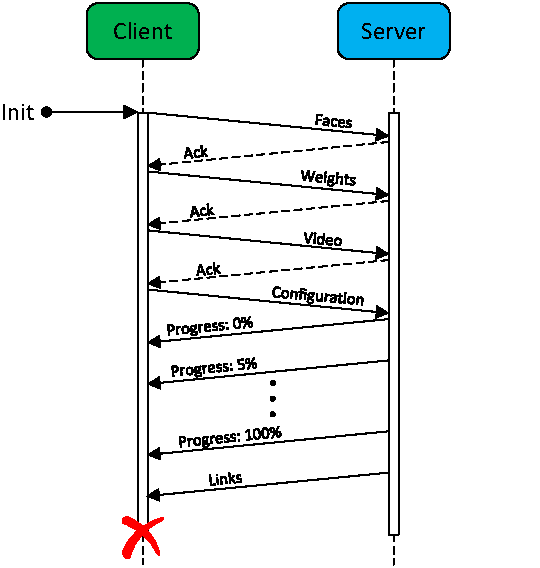
\includegraphics[width=0.8\textwidth]{obrazky-figures/socket_com.pdf}
	\caption{Komunikace mezi klientem a~serverem prostřednictvím Socket.io.}
	\label{img:socketCom}
\end{figure}

Poté, co jsou nahrány všechny snímky je klientská strana o~této skutečnosti informována a~začne posílat soubor s~váhami. Váhy se uloží přímo do dočasného adresáře vedle databáze. Během přenosu je klient informován o~množství přenesených dat, která jsou pak znázorněna pomocí ukazatele. Jakmile jsou váhy kompletně nahrány, tak si k~nim server uloží cestu a~informuje klienta o~dokončeném přenosu. Ten následně začne posílat videozáznam. Celý proces přenosu probíhá stejně jako v~případě vah a~klient je na konci opět informován o~úspěšném dokončení akce.

Následně co klientská strana obdrží zprávu o~dokončeném přenosu videozáznamu, tak odešle data s~konfigurací, kterou uživatel nastavil v~předchozích krocích. Potom co tuto konfiguraci obdrží server, tak ji převede na argumenty python skriptu. Program obsahuje celkem $15$ argumentů a~většina z~nich je převedena pomocí funkce \texttt{parseArgsCLI()} v~souboru \texttt{utils.js}. Kromě uživatelské konfigurace je totiž nutné taky zadat cesty k~nahraným souborům, které si server postupně ukládal. Jakmile je konfigurace převedena na parametry, tak se vytvoří nový proces, který s~těmito parametry spustí program. Vytvoření speciálního procesu pro tento úkon má zásadní vliv na chod serveru, protože celý běh serveru je řízen pouze jedním vláknem a~v~opačném případě by došlo k~jeho zablokování a~znemožnění konkurentního zpracování (viz~sekce~\ref{sec:Node} o~Node.js).

Během toho, co nový proces zpracovává video, tak vypisuje na standardní výstup aktuální postup zpracování. Tento výstup je zachytáván hlavním procesem a~přeposílá ho do klientské části, kde je následně zobrazen. Uživatel je tak neustále informován o~aktuálním průběhu. Poté co skript skončí, tak se ověří jeho návratová hodnota. Návratový kód $0$ indikuje, že video bylo úspěšně zpracováno a~skript uložil zpracovaný záznam do adresáře \texttt{videos} spolu se souborem JSON, ve kterém jsou zaznamenány informace o~detekovaných objektech. Uživatel je informován o~dokončeném zpracování a~jsou mu odeslány odkazy, pod kterými tato data najde. Pokud skript skončil s~nenulovou hodnotou, tak je uživatel informován o~chybě (může způsobit např.~špatný formát vah pro neuronovou síť). Nakonec je celý dočasný adresář klienta odstraněn pomocí funkce \texttt{rmDirRecursive()} implementované v~souboru \texttt{utils.js}, protože nadále již není potřeba a~klient je od serveru odpojen.

Výsledné dva soubory jsou tedy uloženy v~adresáři \texttt{videos} pod identifikátorem klienta. V~této části přichází na řadu Express.js, který je zpřístupní klientovi pomocí běžných bezstavových HTTP metod. Express implementuje v~adresáři \texttt{routes} následující tři cesty:
\begin{itemize}
    \item \texttt{\textbf{video}}~--~Cesta, která pomocí parametru \texttt{ID} vrátí klientovi zpracovaný videozáznam, jenž je použit v~aplikaci pro přehrání.
    \item \texttt{\textbf{download}}~--~Cesta, která pomocí parametru \texttt{ID} umožní klientovi stáhnout zpracovaný záznam.
    \item \texttt{\textbf{data}}~--~Cesta, která pomocí parametru \texttt{ID} vrátí klientovi data s~detekovanými objekty ve formátu JSON, která jsou uživateli zobrazena jako souhrn.
\end{itemize}

Na výpisu~\ref{vyp:jsonSummary} je znázorněna reálná ukázka obsahu JSON souboru s~informacemi o~detekovaných objektech na videu. Soubor obsahuje objekt, kde každý detekovatelný objekt je reprezentován odpovídajícím klíčem. Každý klíč má hodnotu pole, do kterého se ukládají časy v~sekundách, ve kterých došlo k~detekci daného objektu. Detekce osob má však jiný formát, protože je nutné odlišit rozpoznané osoby od těch ostatních.

U osob se do pole místo čísel ukládají další objekty, které reprezentují konkrétní osobu. Každá osoba má unikátní identifikátor, jméno a~pole s~detekcemi, které obsahuje objekty reprezentující konkrétní detekci na záznamu. Objekt detekce pak obsahuje identifikátor, který odpovídá identifikátoru snímku obličeje, vůči kterému byla osoba rozpoznána a~položku s~časy, při kterých k~této události došlo. Pokud osoba bude rozpoznána vůči dvěma snímkům, potom pole s~detekcemi bude obsahovat dva objekty. V~případě, kdy dojde k~opětovnému rozpoznání vůči snímku, který je zde již zaznamenán, tak se přidá pouze další čas do odpovídajícího objektu podle \texttt{ID}. Osoba, jejíž \texttt{ID} je prázdný řetězec pak reprezentuje ostatní osoby, které nebyly rozpoznány a~obsahuje právě jednu detekci pro zaznamenání časů. Důležité je poznamenat, že čas bude uložen pouze pokud k~dané detekci došlo naposledy nejméně před $5$-ti sekundami, jinak by docházelo k~nadbytečnému ukládání dat či redundancím.

Zpracovaná data jsou na serveru dostupná po dobu $24$ hodin, než dojde k~jejich odstranění. O~tuto činnost se stará funkce \texttt{deleteFiles()} implementovaná v~souboru \texttt{utils.js}, která je volána každou hodinu a~prochází adresář \texttt{videos}. V~adresáři postupně kontroluje metadata každého souboru a~pokud je soubor starší více než $24$ hodin, tak ho smaže.

\newpage
\begin{lstlisting}[language=json,firstnumber=1, label={vyp:jsonSummary}, caption={Ukázka obsahu JSON souboru s~informacemi o~detekovaných objektech ve videu.}]
{
  "person": [
    {
      "id": "",
      "name": "Unknown",
      "detections": [
        {
          "id": "",
          "last": 1,
          "timestamp": [
            0
          ]
        }
      ]
    },
    {
      "id": "8",
      "name": "Jenny Williams",
      "detections": [
        {
          "id": "6",
          "last": 1,
          "timestamp": [
            0
          ]
        }
      ]
    }
  ],
  "car": [
    0
  ],
  "cat": [],
  "dog": [],
  "horse": [],
  "sheep": [],
  "cow": [],
  "elephant": [],
  "bear": [],
  "zebra": [],
  "giraffe": []
}
\end{lstlisting}

\section{Zpracování videozáznamu}
Po spuštění programu pro zpracování videa dojde nejdříve k~inicializaci objektů \texttt{Detector}, \texttt{Recognizer}, \texttt{Tracker} a~\texttt{Recorder}, které budou následně zodpovědní za detekci objektů, rozpoznávání osob, sledování a~zaznamenávání detekcí na záznamu. Celý proces zpracování je abstraktně znázorněn na konci této sekce v~algoritmu~\ref{alg:ProcesZpracováníVidea} a~ukázku zpracovaného snímku lze vidět na obrázku~\ref{img:videoSample}. Objektu třídy \texttt{Detector} je při inicializaci nutné předat seznam s~třídami detekovatelných objektů a~specifikovat cestu ke konfiguračnímu souboru a~předtrénovaným vahám YOLOv3 (viz~sekce~\ref{sec:YOLO}). V~adresáři \texttt{yolov3} jsou uloženy dva konfigurační soubory, které se liší v~rozlišení snímků, které budou vkládány do neuronové sítě. Lze vybrat mezi dvěma rozlišeními~--~$320\times320$ a~$608\times608$, jaká konfigurace se však použije rozhoduje uživatel argumentem programu (výchozí je $320\times320$).

\begin{figure}[hbt]
	\centering
	\setlength{\fboxsep}{0pt}
	\includegraphics[width=1.0\textwidth]{obrazky-figures/video_sample.png}
	\caption{Ukázka snímku ze zpracovaného videa, na kterém se nachází detekována osoba, jenž vchází do sledované oblasti na příjezdové cestě. Za osobou je vykreslená stopa, která zobrazuje trasu odkud přišla a~zároveň je zobrazeno její jméno, které bylo zjištěno při rozpoznání obličeje v~předchozí části videa.}
	\label{img:videoSample}
\end{figure}

Při inicializaci objektu třídy \texttt{Recognizer} je nutné definovat cestu k~adresáři se snímky obličejů, které mají být použity pro identifikaci. Rozpoznávání je prováděno pomocí systému DeepFace (viz~sekce~\ref{sec:DeepFace}) na modelu Facenet. \texttt{Tracker} je implementovaný na algoritmu DeepSORT (viz~sekce~\ref{sec:DeepSORT}), který je uložený v~adresáři \texttt{deep\_sort} a~při jeho inicializaci se pouze nastavují parametry jako maximální stáří sledovaných objektů, práh shody, doba mezi aktualizacemi měření a~další. Hodnoty těchto parametrů byly testovány na různých záznamech a~napevno nastaveny tak, aby došlo k~rovnováze mezi častou záměnou identifikátorů a~jejich chybnému přiřazení. Objekt třídy \texttt{Recorder} se používá pouze k~zaznamenávání detekovaných objektů a~při inicializaci je nutné mu předat seznam detekovatelných tříd, podle kterých vytvoří strukturu, do které bude zaznamenávat časy.

\newpage
Poté co jsou inicializovány nejdůležitější komponenty pro zpracování videa, tak se otevře zdrojové video a~získají se z~něj metadata, která se použijí pro zápis zpracovaného videa, výpočtu aktuálního času~aj. Cílové video bude uloženo do adresáře specifikovaného v~argumentu programu ve formátu \texttt{.mp4} s~kodekem H.264\footnote{OpenH264: \url{https://github.com/cisco/openh264}}. Tento kodek byl vybrán kvůli jeho široké podpoře napříč prohlížeči a~při zobrazení výsledného videa ve webovém přehrávači by tedy neměl nastat žádný problém. Rozlišení videa a~jeho snímková frekvence je pak stejná jako u~zdrojového videa, ačkoliv by mohlo dojít ke značné redukci za účelem snížení časové náročnosti. Zachování těchto vlastností je ze strany uživatele na první pohled očekávané a~z~toho důvodu nedochází k~žádné modifikaci.

Celý proces zpracování běží ve smyčce přes všechny snímky ve videu~--~viz~algoritmus~\ref{alg:ProcesZpracováníVidea}. Nad každým snímkem se nejdříve zavolá funkce \texttt{predict()} objektu \texttt{detector}, která vrátí třídy, bounding boxy a~confidence skóre všech nalezených objektů. Funkce jako první převede snímek s~přehozeným červeným a~modrým kanálem barev na \emph{blob}, který následně vloží na vstup neuronové sítě. Z~výstupních vrstev YOLOv3 se poté posbírají predikce, které se vyfiltrují pomocí techniky Non-Maximum Suppression za účelem eliminace překrývajících se bounding boxů, které ohraničují ten samý objekt. Z~vyfiltrovaných detekcí se pak vytvoří seznam objektů třídy \texttt{Detection}, jenž reprezentuje konkrétní detekci na snímku a~uchovává její data.

Pokud je aktivován modul pro rozpoznávání osob, tak u~každé detekce, která byla klasifikována jako osoba dojde k~vyříznutí odpovídajícího bounding boxu ze snímku a~předá se funkci \texttt{find()} objektu \texttt{recognizer}. Funkce provede identifikaci a~vrátí jméno osoby, naměřenou vzdálenost, identifikátor osoby a~obličeje. Jméno a~identifikátory jsou získány z~názvu snímku obličeje, podle kterého byla osoba rozpoznána (viz~formát uložených snímků v~sekci~\ref{sec:server}). Pokud nedojde k~žádné shodě, tak je jméno osoby nastaveno na \emph{Unknown} a~naměřená vzdálenost je rovna $1$. Tato data se pak přiřadí k~detekci pomocí funkce \texttt{setIdentity()}.

Následuje modul pro sledování objektů, který se aktivuje pouze v~případě, pokud byl nastavený odpovídající argument programu. Celý proces je proveden ve funkci \texttt{track} objektu \texttt{tracker}, která bere jako parametry aktuální snímek a~seznam detekcí. Zde je ze začátku nutné převést objekty ze třídy \texttt{Detection} na objekty reprezentující detekci, které používá DeepSORT. Ten kromě základních údajů také vyžaduje reprezentaci detekce pomocí mapy příznaků, kterou používá ke sledování (porovnání) objektů napříč snímky. Zároveň je žádoucí také uchovat informace o~identitě osoby, barvy bounding boxu~aj. Z~těchto důvodů bylo nutné upravit následující soubory DeepSORTu:
\begin{itemize}
    \item \texttt{\textbf{detection.py}}~--~Třída reprezentuje detekci. Při inicializaci byly přidány parametry a~atributy pro uchování dalších dat.
    \item \texttt{\textbf{track.py}}~--~Implementuje třídu, která reprezentuje danou stopu. Opět je zde potřebné přidat při inicializaci parametry a~atributy pro uchování dat. Ve funkci \texttt{update()}, která přijímá jako parametr novou detekci byla doplněna logika pro aktualizaci atributů během existence daného objektu. Např.~confidence skóre a~třída se pokaždé aktualizují, ale identita osoby se přepíše pouze pokud nová identita obsahuje lepší naměřenou vzdálenost a~zároveň pokud je splněný minimální práh pro aktualizaci.
    \item \texttt{\textbf{tracker.py}}~--~Ve třídě \texttt{Tracker} je na konci pouze doplněné předávání dat z~detekce do stop při její inicializaci.
\end{itemize}

Potom co DeepSORT spočítá z~detekcí nový stav stop, tak se všechny potvrzené stopy převedou opět na původní objekty třídy \texttt{Detection} a~budou navíc doplněné o~identifikátor a~seznam středových bodů předchozích bounding boxů, jenž slouží pro vykreslování cest. To se provádí jednoduchým propojením bodů úsečkami od aktuální pozice postupně ke starším bodům. Počet propojených bodů je specifikován argumentem programu, který definuje po jaké době se cesty už nemají vykreslovat. Je tedy nutné počet bodů spočítat pomocí tohoto argumentu v~závislosti na snímkové frekvenci videa.

V tomhle okamžiku jsou získána všechna data o~objektech na aktuálním snímku. Před samotným vykreslením je ale potřeba ošetřit, jestli detekované objekty patří mezi objekty, které mají být na snímku vykresleny, protože předtrénovaná síť YOLO na datasetu COCO detekuje 80 různých tříd. Kromě toho takové automobily se detekují potom, co je nastavený odpovídající argument programu. Dále také program umožňuje specifikovat detekční oblast a~do této doby se detekce prováděla na celém snímku. Je tedy nezbytné zároveň ošetřit, jestli detekce, která má být vykreslena, se nachází uvnitř této oblasti porovnáním hraničních hodnot oblasti a~souřadnic středového bodu bounding boxu.

Detekce se po vykreslení zaznamenají do objektu třídy \texttt{Recorder}, který na konci procesu vygeneruje souhrn všech nálezů ve formátu JSON a~jeho formát je popsán v~předchozí sekci~\ref{sec:server}. V~poslední části, pokud bylo nastavené počítání objektů, se na snímek vykreslí počítadlo s~přítomnými objekty, jehož hodnota je dána počtem aktuálních detekcí, jejichž třída patří mezi detekovatelné objekty a~nachází se uvnitř detekční oblasti. Hodnota počítadla s~celkovým počtem objektů je pak dána mohutností množiny, do které se postupně ukládají identifikátory těchto detekcí. Pokud je nastaveno i~vykreslení detekční oblasti nebo času na snímek, tak dojde k~jejich vykreslení. Tento proces se následně opakuje na všech snímcích ve videu.

\begin{algorithm}
\caption{Proces zpracování videa}
\label{alg:ProcesZpracováníVidea}
\begin{algorithmic}[1]
\Procedure{ProcessVideo}{$args, videoPath, destPath, detectableObjects$}
    \State $detector \gets YOLOv3$    \Comment{Inicializace}
    \State $recognizer \gets DeepFace$
    \State $tracker \gets DeepSORT$
    \State $recorder \gets \{object$: list() \textbf{for each} $object \in detectableObjects\}$
    \State $video \gets$ videoReader($videoPath$)     \Comment{Načtení videa}
    \State $output \gets$ videoWriter($destPath$)

    \State
    \ForEach {$frame \in video$} \Comment{Zpracování každého snímku}
        \State $classes, confs, bboxes \gets detector$.predict($frame$) \Comment{Detekce}
        \State $detections \gets$ list()
        \ForEach {$class, conf, bbox \in$ zip($classes, confs, bboxes$)}
            \State $detections$.append(Detection($class, conf, bbox$))
        \EndFor
        \If{$args.recognition$ == \texttt{True}}    \Comment{Identifikace}
            \ForEach {$detection \in detections$}
                \If{$detection.class$ == \texttt{"person"}}
                    \State $crop \gets$ imageCrop($frame, detection.bbox$)
                    \State $identity, faceDist, personId, faceId \gets recognizer$.find($crop$)
                    \State $detection$.setIdentity($identity, faceDist, personId, faceId$)
                \EndIf
            \EndFor
        \EndIf
        \If{$args.tracking$ == \texttt{True}}    \Comment{Sledování objektů}
            \State $detections \gets tracker$.track($frame, detections$)
        \EndIf
        \ForEach {$detection \in detections$}   \Comment{Vykreslení detekcí}
            \If{$detection.class$ == \texttt{"car"} $\land$ $args.cars$ == \texttt{"False"}}
                \State continue
            \EndIf
            \If{$detection.class \in detectableObjects$}
                \If{$args.area$ == \texttt{None} $\lor$ $detection.bbox \in args.area$}
                    \State drawDetection($frame, detection$)
                    \State $recorder$.add($detection$)
                \EndIf
            \EndIf
        \EndFor
        \If{$args.area \neq$ \texttt{None} $\land$ $args.frame$ == \texttt{True}} \Comment{Vykreslení oblasti}
            \State drawRect($frame, args.area$)
        \EndIf
        \If{$args.tracking$ == \texttt{True} $\land$ $args.counters$ == \texttt{True}} \Comment{Počítadla}
            \State drawCounters($frame, detections, args.area$)
        \EndIf
        \If{$args.timestamp$ == \texttt{True}} \Comment{Vykreslení aktuálního času}
            \State drawTime($frame, video.position, video.fps$)
        \EndIf
    \EndFor
    \State $recorder$.saveJSON($destPath$)
\EndProcedure
\end{algorithmic}
\end{algorithm}


\chapter{Experimenty a~vyhodnocení systému}
\label{kap:experimenty}
V poslední části bylo provedeno měření za účelem vyhodnocení kvality a~použitelnosti celého systému. Veškerá dále uvedená data byla naměřena na reálných záznamech z~kamer na sestavě, která disponovala procesorem značky Intel Core i7-7700HQ s~frekvencí $2,80$~GHz a~operační pamětí $8$~GB. Kromě toho tato kapitola obsahuje popis, podle kterého byl při implementaci zohledněn výběr detektoru z~pohledu jeho přesnosti.

\section{Vyhodnocení výkonnosti}
Výkonností řešení se v~tomto kontextu myslí potřebný čas ke zpracování jednoho záznamu, jelikož právě to nejvíce ovlivňuje uživatele a~použitelnost celého systému v~praxi. Existuje mnoho faktorů, které tuto dobu ovlivňují, jako je např.~množství aktivovaných operací v~konfiguraci, snímková frekvence videa nebo hardwarové vybavení serveru. V~předchozí kapitole~\ref{kap:implementace} bylo řečeno, že mezi hlavní komponenty, které majoritně ovlivňují dobu zpracování patří detekce, identifikace osob a~sledování objektů, proto v~rámci měření byly tyto časy zaznamenávány odděleně.

Doba k~provedení detekce je dána výkonností neuronové sítě YOLOv3 a~na neštěstí je značně ovlivněna počtem detekovatelných objektů, přičemž značná část nemá v~řešení využití. Na druhou stranu potřebný čas k~provedení této operace při rozlišení $320\times320$ je poměrně malý, tj.~průměrně {\raise.17ex\hbox{$\scriptstyle\sim$}}$294$ ms na CPU. Čas je dále možné značně zredukovat akcelerací pomocí GPU, kde průměrný čas na snímek dosahuje {\raise.17ex\hbox{$\scriptstyle\sim$}}$63$ ms na grafické kartě GTX $1050$Ti s~pamětí $4$~GB a~v~tomto případě bylo tak dosaženo {\raise.17ex\hbox{$\scriptstyle\sim$}}$4,7$násobného zrychlení (viz~graf~\ref{img:cpuVSgpu}).

\begin{figure}[hbt]
	\centering
	\setlength{\fboxsep}{0pt}
	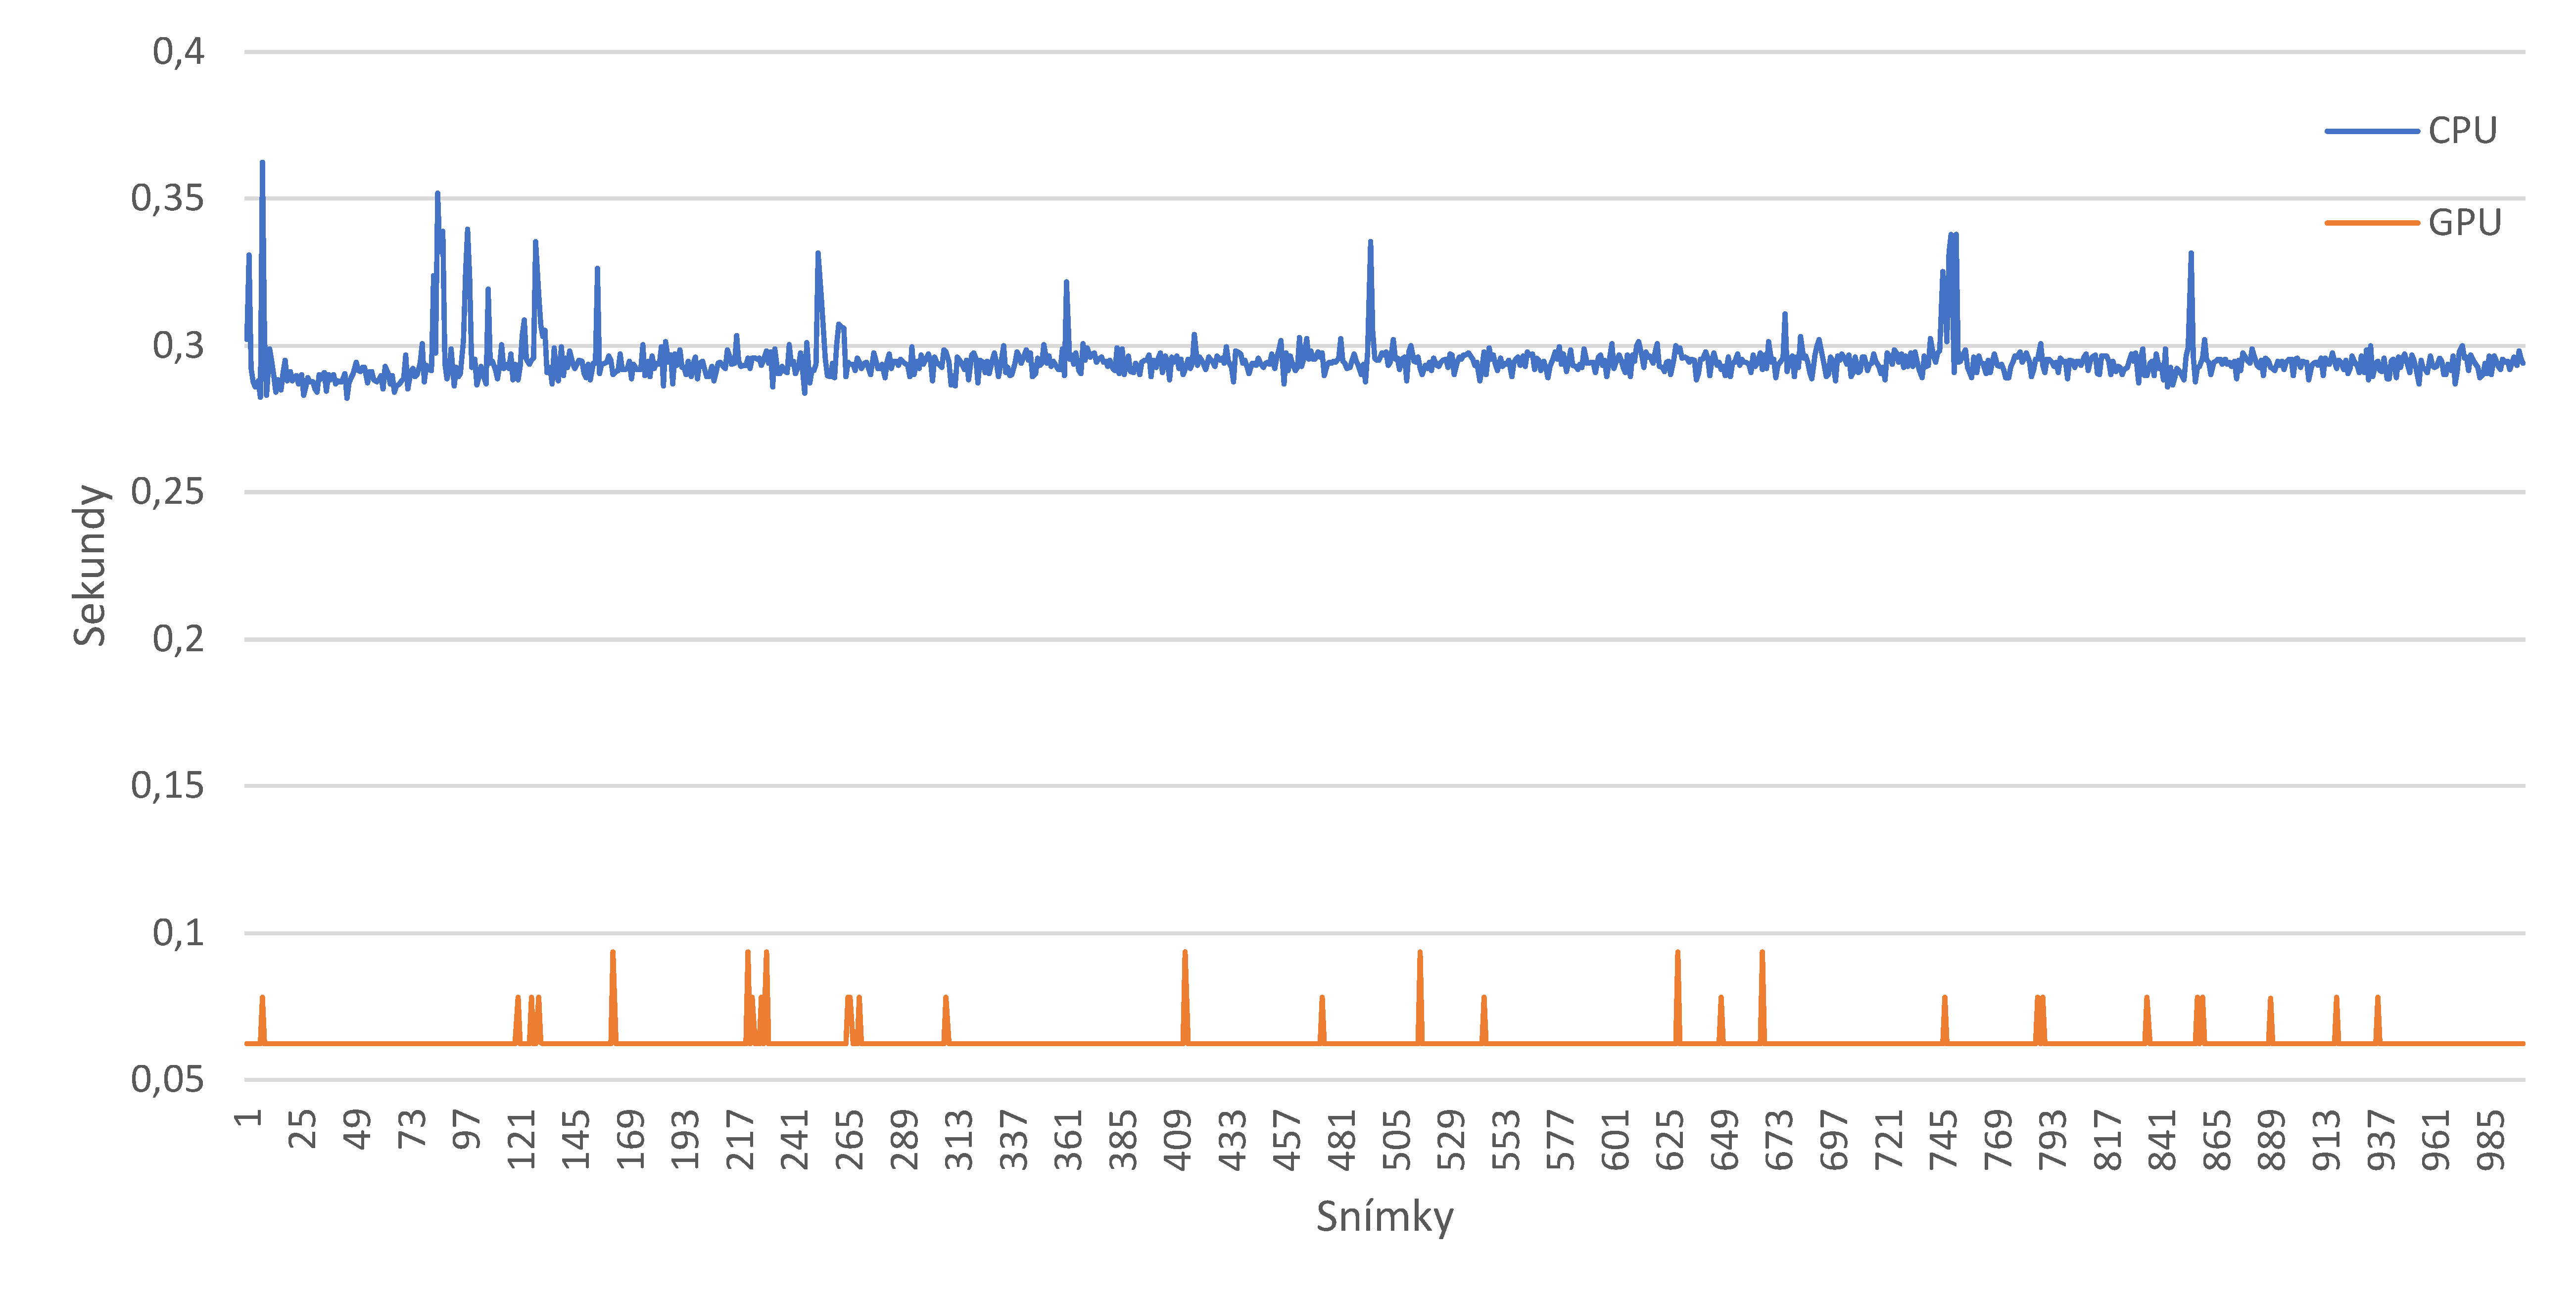
\includegraphics[width=1.0\textwidth]{obrazky-figures/detection_cpu_gpu_times.pdf}
	\caption{Časy pro detekci objektů na 1000~snímcích pomocí procesoru Intel Core i7-7700HQ $2,80$~GHz a~grafické karty GTX $1050$Ti $4$GB, kde grafická karta vykazuje znatelně lepší výsledky.}
	\label{img:cpuVSgpu}
\end{figure}

Identifikace osob je provedena pouze v~případě, pokud byla osoba v~první řadě na snímku detekována. Nelze tedy říci, že tento modul bude zatěžovat celý průběh zpracování záznamu, protože v~případě, kdy se na snímku nenachází žádná osoba, tak dochází k~nulovému zpoždění. Přičemž se dá očekávat, že na skutečném záznamu, ve kterém se vyskytují narušitelé jen výjimečně, tak nebude docházet k~aktivaci příliš často. Nicméně průměrný čas pro identifikaci osoby pomocí systému DeepFace z~naměřených hodnot na CPU zabere {\raise.17ex\hbox{$\scriptstyle\sim$}}$60$ ms (viz~graf~\ref{img:cpuTimes}). Jelikož jsou osoby rozpoznávány jednotlivě, tak výsledný čas také záleží na množství osob, které se na daném snímku nachází, tedy v~případě čtyř osob bude pak celkové zpoždění $4 \cdot 60 = 240$ ms.

\begin{figure}[hbt]
	\centering
	\setlength{\fboxsep}{0pt}
	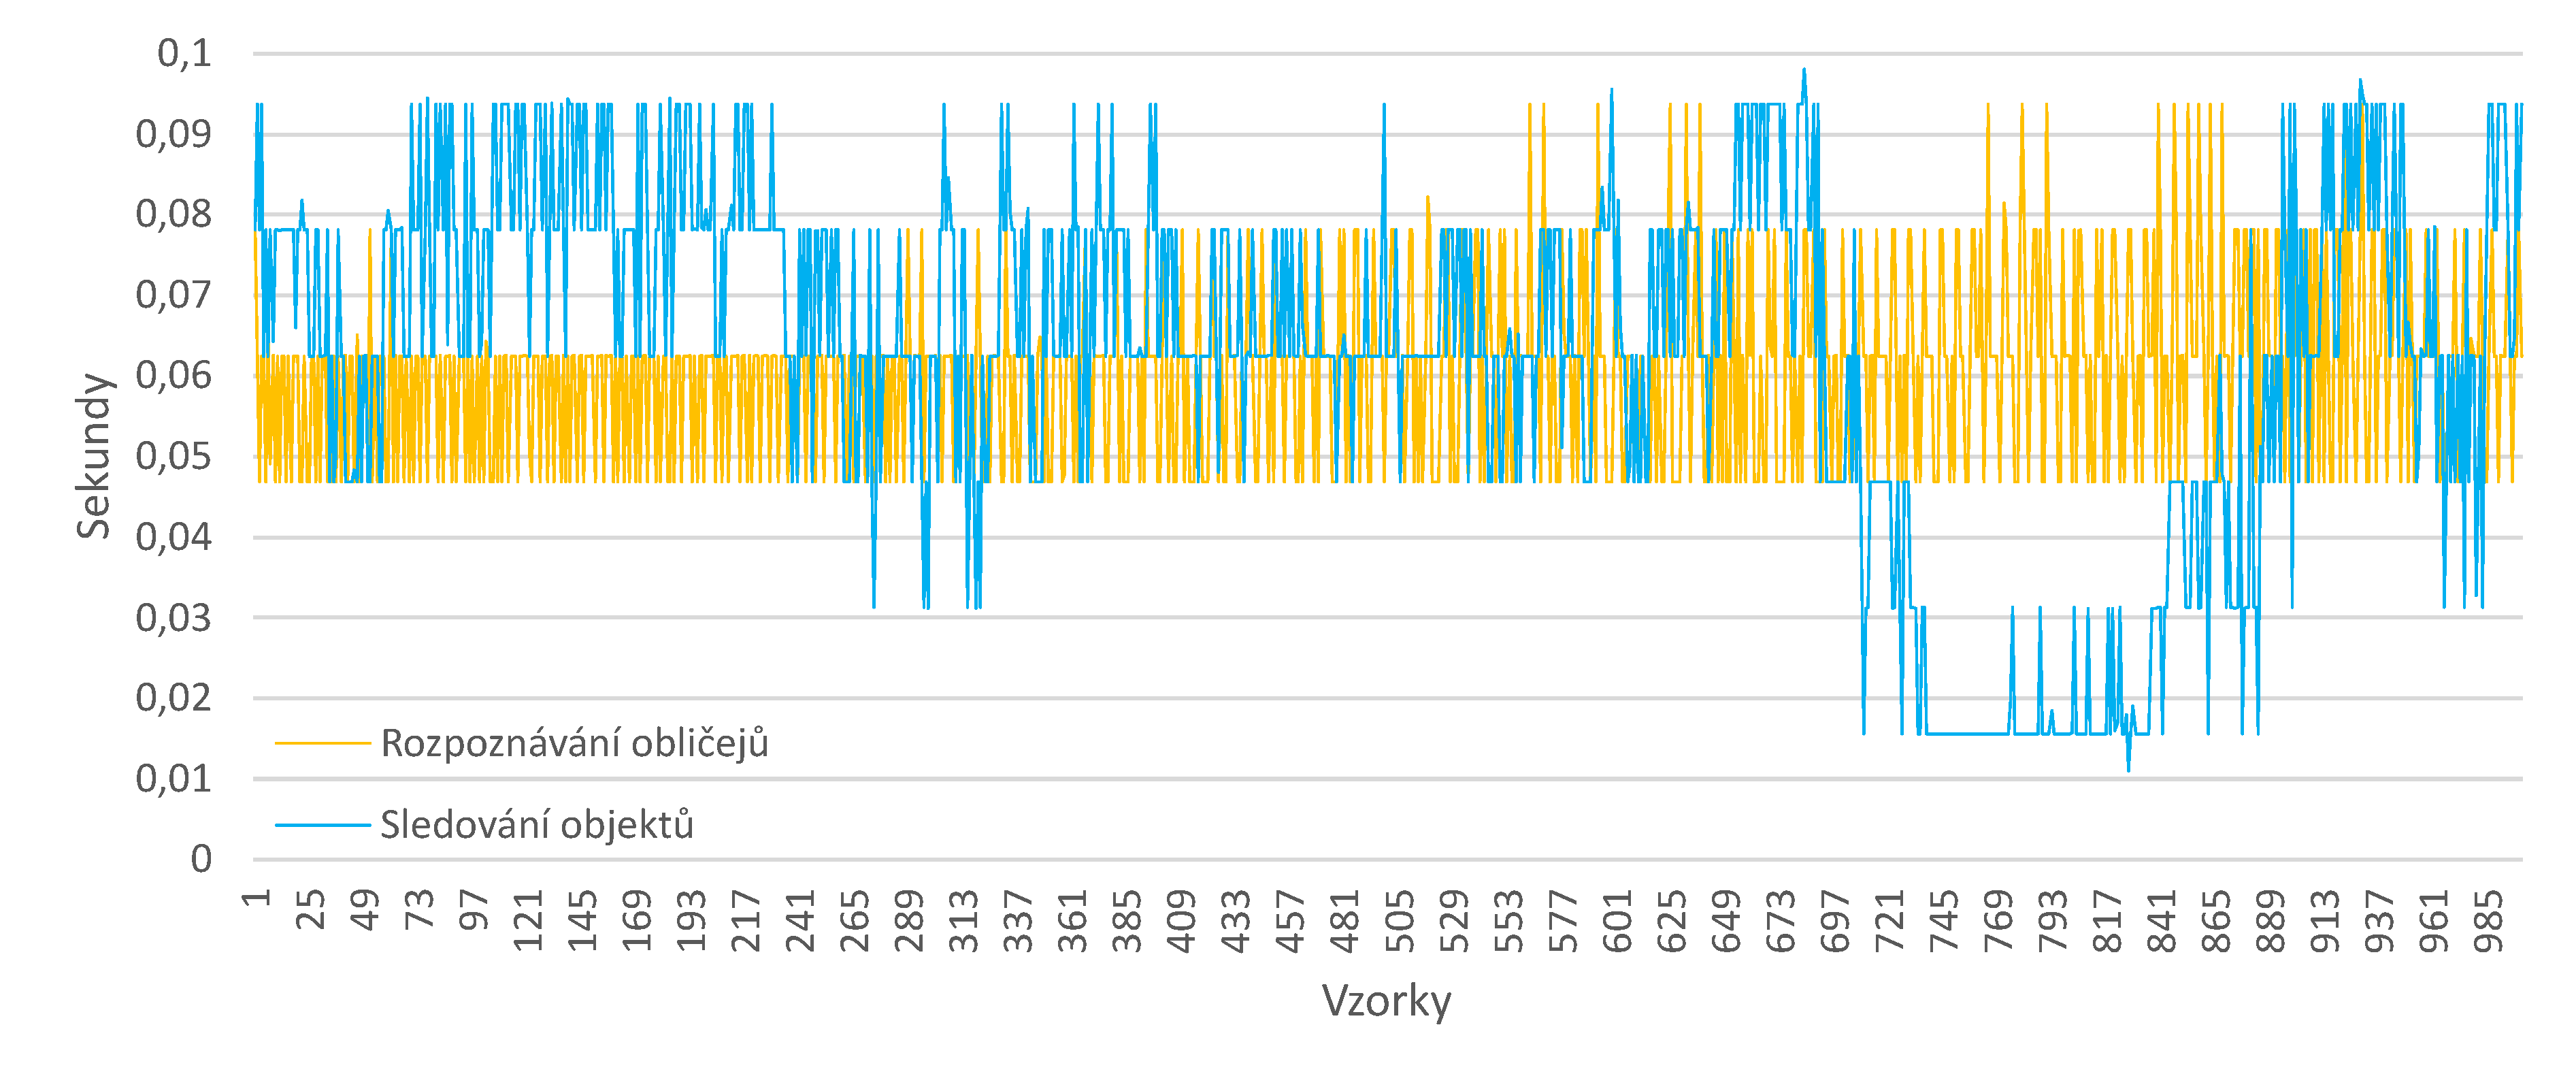
\includegraphics[width=1.0\textwidth]{obrazky-figures/recognition_tracking_times.pdf}
	\caption{Časy pro identifikaci jedné osoby podle obličeje a~sledování detekovaných objektů na jeden snímek. Naměřeno na 1000~vzorcích.}
	\label{img:cpuTimes}
\end{figure}

Pokud je nastavené sledování objektů, tak je tato operace stejně jako detekce provedena na každém snímku a~značně se tak podílí i~na celkové době zpracování. Ovšem DeepSORT, umožňuje zpracování v~reálném čase a~z~naměřených hodnot pak vychází průměrná hodnota {\raise.17ex\hbox{$\scriptstyle\sim$}}$62$ ms na jeden snímek (viz~graf~\ref{img:cpuTimes}), což se stále dá považovat za přijatelný výsledek.

Pro ilustraci lze uvážit zpracování $5$minutového videa, kde při výpočtu je zanedbána identifikace osob, protože je definovaná obsahem na záznamu a~značně by tak zkreslovala výsledek. Pokud detekce pomocí GPU zabere $63$ ms a~sledování objektů $62$ ms, potom jeden snímek potrvá zpracovat $63 + 62 = 125$ ms. Při snímové frekvenci $20$ pak zpracovat $1$ sekundu záznamu zabere $125 \cdot 20 \div 1000 = 2,5$ sekund a~celý záznam poté $12,5$ minut. Výsledné zpomalení je $12,5 \div 5 = 2,5$, pokud by tento $5$minutový záznam ovšem měl poloviční snímkovou frekvenci, pak by jeho zpracování zabralo pouhých $6,25$ minut.

\section{Vyhodnocení přesnosti}
Dosažení vyššího výkonu zajištěním co nejkratšího času na provedení detekce objektů přímo ovlivňuje její přesnost. V~rámci řešení bylo vyzkoušeno více detektorů jako je např.~SSD či Faster-RCNN s~ResNet-50~aj. za účelem najít rovnováhu mezi přesností a~dobou zpracování. Detekce jako první operace tak značně ovlivňuje další zpracování a~její přesnost rozhoduje např.~o~tom, zda osoby pak budou vůbec rozpoznány či správně sledovány. Osobu totiž nelze nijak rozpoznat pokud daný bounding box neobsahuje její obličej. Časté výpadky při detekci objektu pak zapříčiňují špatnou asociaci s~jeho předchozí polohou.

Při experimentech byla použita např.~síť YOLOv3-tiny, která nabízí vysokou rychlost zpracování. Na CPU dosáhla průměrné rychlosti detekce $52$ ms na snímek při nastaveném rozlišení $416 \times 416$ a~tím umožnila $5,65$krát rychlejší detekci než běžné YOLOv3 při rozlišení $320\times320$. Ovšem s~detekovanými objekty z~této sítě již není možné dále v~řešení pracovat (viz~obrázek~\ref{img:accuracy}). V~tomto případě jsou bounding boxy objektů velmi nepřesné, osoby jsou detekovány bez obličejů, dochází k~velkému množství výpadků a~chybných detekcí (nízké confidence skóre). Z~oficiální dokumentace tato síť poskytuje mAP \emph{(mean average precision)} $33,1$. Z~toho důvodu byl použit detektor YOLOv3 při rozlišení $320\times320$ jako nejrychlejší možnost, protože s~těmito detekcemi lze s~jistotou dále pracovat a~jeho mAP dosahuje $51,5$, při rozlišení $608 \times 608$ bylo pak mAP naměřeno na $57,9$.

\begin{figure}[hbt]
	\centering
	\setlength{\fboxsep}{0pt}
	\includegraphics[width=1.0\textwidth]{obrazky-figures/yolo_accuracy.png}
	\caption{Porovnání detekce osob pomocí YOLOv3-tiny s~rozlišením $416 \times 416$ (vlevo) a~YOLOv3 při rozlišení $320\times320$ (vpravo), kde YOLOv3-tiny nabízí mnohonásobně větší rychlost zpracování, ovšem detekce jsou velmi nepřesné a~některé zcela chybí.}
	\label{img:accuracy}
\end{figure}


\chapter{Závěr}
Zadáním této práce bylo nastudovat problematiku detekce a~klasifikace objektů v~obraze a~následně se zaměřit na aktuální řešení pro rozpoznávání osob podle obličeje. Dále pak navrhnout a~implementovat řešení pro detekci a~analýzu narušitelů ve sledované oblasti v~podobě klient-server aplikace. Celý systém otestovat na reálných záznamech a~nakonec zhodnotit jeho praktické nasazení.

Nastudovaná teorie byla v~tomto textu sepsána obecným úvodem do oblasti neuronových sítí, jenž má za úkol uvést čtenáře do kontextu práce. O~ten se pak opírá následující sekce o~konvolučních neuronových sítích, které se používají pro zpracování obrazu. Následně byly uvedeny některé páteřní architektury a~detektory pro detekci a~klasifikaci objektů. Další část textu pak byla věnována detekci obličejů, vybraným přístupům pro rozpoznávání osob a~metodám pro sledování objektů. V~rámci teoretické části byly také popsány technologie, které byly použity při implementaci výsledné aplikace.

Po návrhu řešení v~rámci praktické části byl nejdříve implementován skript pro zpracování videozáznamu, po kterém byla následně vytvořena klientská a~serverová část celého systému. Po integraci všech těchto částí vznikla použitelná aplikace pro detekci narušitelů s~možností konfigurace, která je schopna spolehlivě zpracovávat záznamy od více uživatelů současně. Aplikace nabízí kromě identifikace osob řadu dalších užitečných funkcí jako je vymezení sledované oblasti, sledování a~počítání objektů, vykreslování cest, uplatnění vlastního detektoru, modifikaci přesnosti a~mnoho dalšího. Výsledky je pak umožněné sdílet mezi uživateli pomocí odkazu. Aplikace byla nakonec otestována na reálných záznamech a~naměřené hodnoty byly vyhodnoceny.

Jako navazující rozšíření této práce by bylo možné přidat do konfigurace zpracování další funkce, které by uživatel mohl v~rámci detekce narušitelů využít. Mezi takové funkce by mohl patřit zejména odhad výšky osob nebo jejich pozice v~prostoru. Získané pozice by se pak odesílaly zpět ke klientovi obdobně jako současný souhrn narušitelů, kde by byly vyneseny např.~v~interaktivní 3D scéně. Pokud by však aplikace měla mít širší využití, tak při současné koronavirové situaci by mohla najít využití funkce pro měření vzdálenosti mezi osobami, kde by při blízkém kontaktu došlo k~zaznamenání zvláštní události.
